\section{Background}
This section presents a review of existing algorithms, an anomaly taxonomy, and an evaluation of existing anomaly detection libraries. Additionally, this section includes an overview of the Work Packages (WPs) that define the deliverables of the FIREMAN project.

\subsection{FIREMAN Work Packages}
\label{ref_FIREMAN_WP}

This subsection outlines the progress and overall goal of the milestones or work packages that guide the FIREMAN project. The interconnection and overview of the individual WPs is shown in Figure \ref{fig:wp-diagram}

\begin{figure}[H]
    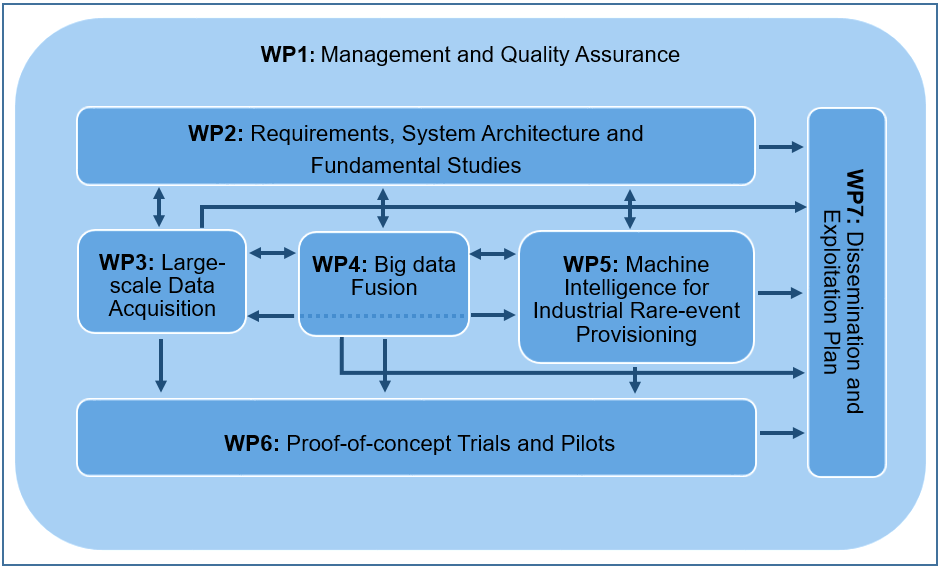
\includegraphics[width=\textwidth]{Images/FIREMAN_pert_diagram.png}
    \caption{FIREMAN WP Diagram \parencite{fireman-homepage}}
    \label{fig:wp-diagram}
\end{figure}

This work focuses on WP6 discussed in Section \ref{ref_wp6} by demonstrating an implementation of a theoretical algorithm for real-world anomaly detection.

\subsubsection{Large Scale Data Acquisition (WP3)}

This work package focuses on \enquote{event-based modelling and traffic characterization techniques aiming for a reduced use of communication and storage resources.
This pre-processing task is expected -among others- to optimize the subsequent data transmissions by injecting only relevant data in the network to reduce overhead and increase spectral efficiency.} \citel{wp3.1}

In this portion of FIREMAN, we examined a  variety of industrial datasets including the Tennessee Eastman Process, Electricity Metering, IEC-61850 Distribution Automation, and the EPFL Smart Grid Pilot.
This dataset is not heavily reliant on relational constraints or atomicity, consistency, isolation, durability (ACID) compliance.
Because of this, we have selected a non-relational PostgreSQL database for storage because of its superior throughput and increased performance in data processing applications.

The sensors traditionally used in Cyber-Physical Systems do not have much compute or storage capacity which makes pre-processing of data at the sensor level challenging.
Because of this, \enquote{compression is essential for reducing the challenge of data storage, collection, transmission, processing, and analysis at the local level}\parencite{compression}.
Authors \cite{wp3.2} have shown that it is possible to achieve a 92.6\% compression rate which means that only 7.4\% of samples are transmitted.
We have also used different methods including linear interpolation to de-compress the data and have measured the error using the root mean square technique.

Modeling of transmission reduction techniques are centered around the electricity modeling dataset \parencite{elect-model-dataset-9694611}.
Three approaches for reducing transmissions were presented including transmissions on large spikes, transmissions on accumulated variance, and time interval defined transmissions with a timeout to compensate for meter or network failure.
These simulations have shown a large potential for reducing transmissions without significantly affecting the accuracy of the measured signal.
We modeled a Markov-Modulated Poission Process to simulate these industrial processes for use in further stages of the project.

\subsubsection{Big Data Fusion (WP4)}
\label{ref_wp4}
The goal of this task is \enquote{to show how a large number of sensors and their corresponding data can be  accommodated and aggregated at small cost for reliably detecting rare events}\parencite{wp4.1}.
This task focuses on three primary objects:
\begin{inlinelist}
    \item heterogeneous data aggregation in machine-type communications;
    \item signature-based cluster formation; and
    \item IoT platform and database selection.
\end{inlinelist}

Data aggregation is important because it is challenging to simultaneously connect a massive number of devices.
This strategy outlined by Authors \cite{massive-machine} relies on the following principals:
\begin{inlinelist}
  \item decreasing communication distance and power consumption of connected devices;
  \item utilizing an efficient distributed node routing network to decrease bandwidth congestion of central nodes; and
  \item extending the network coverage.
\end{inlinelist}
The researchers also introduced a cluster formation scheme based on signatures that reduces the signalling overhead required for peer-discovery in the network. This technique utilizes signal aggregates to reduce traffic congestion to the central node.

Additionally, we surveyed IoT experts to determine the most important properties and components of an IoT system.
This survey compared the five most popular cloud IoT providers: AWS, Azure, GCP, IBM Watson, and Oracle IoT to create a comparison that can be used by businesses when selecting a cloud provider that suits their business needs \parencite{choose-iot-9110590}.

SEAT, an automotive component manufacturer, provided two use cases and accompanying datasets for the FIREMAN project.
The first involves early failure detection of mechanical components in the drive chain in the Paint shop which causes axial displacement.
The second involves detecting early failure of the spindle on a CNC machine which ensures lineal movement over a surface.
In both of these situations, detecting failure early helps SEAT solve problems before they begin to impact production components.
This can eventually reduce production downtime to zero.

\subsubsection{Machine Intelligence for Industrial Rare-event Provisioning (WP5)}

The goal of this task is to utilize machine intelligence techniques to predict indicators of health for a machine, component, or entire industrial process to detect premature failure.
The main technique proposed in this task is the Quantitative Association Rule Mining Algorithm (QARMA).

\enquote{QARMA is a family of algorithms for extracting all (or, depending on user inputs, an important subset of) valid non-dominated quantitative association rules that hold in a dataset, that can then be used for further data analysis such as deriving rule-based classifier ensembles or as explainers of classification results of other black-box classifiers.}\citel{wp5.1}  This technique is one of the most human understandable techniques for machine intelligence and has shown promise for this application. In this WP, QARMA is tested on the SEAT dataset discussed in Section \ref{ref_wp4}.

Traditional methods for pruning the rules created by the algorithm were analyzed in this WP as many of them can be extraneous or unreliable. The fastest open source Mixed-Integer Programming (MIP) tool was able to solve this problem in 19 seconds while the parallelized hybrid search algorithm proposed in this WP solved the problem 240 times faster when using parallel threads.

Authors \cite{wp5.1} used a breadth first search approach to compute a `small' subset of the rules extracted by QARMA that cover the majority of instances in a training dataset. Through experimentation on a synthetic power grid fault diagnostic dataset, QARMA performs better than certain neural networks with noisy data \parencite{ml-performance-power-trans}. This is because of the over-fitting of training data with Deep Neural Network architectures. The rule based methods generated by QARMA produce human understandable rules which is beneficial in creating explainable AI.

\subsubsection{Proof-of-Concept Trails and Pilots (WP6)}
\label{ref_wp6}

The primary objectives of this task as stated by Authors \parencite{wp6.1} using FIREMAN approaches are:
\begin{inlinelist}
    \item testing and deployment of theoretical techniques presented thus far;
    \item specific proof-of-concept demonstrations and simulations ; and
    \item implementation plans for production, real-time monitoring.
\end{inlinelist}

Authors \parencite{wp6.3} describe the Power Electronic Converter (PEC) setup at Aalborg University (AAU) that is discussed in this work. The test setup facilities studying microgrids and the impact of disturbances or faults on power transmission and reliability. With the test setup, it is possible to perturb system parameters and measure their impact on the overall system with various sensor measurements. These simulation conditions are used to create the PEC dataset discussed in Section \ref{ref_pec_dataset}.

\subsection{Algorithm Explainability}

Certain high-risk use cases for machine learning algorithms demand a high level of explainability and confidence in the algorithm outputs to use in decision making. In many cases an algorithm makes a classification decision but there is not a clear explanation as to why. In the field of power electronics, understanding why a data-driven controller is making a decision is critical to incorporating it into real world power distribution scenarios.

\subsubsection{Types of Uncertainty}
Determining sources of uncertainty in a model or system is critical. When analyzing uncertainty, it is important to understand the two different types:
\begin{inlinelist}
    \item epistemic and
    \item aleatoric uncertainty.
\end{inlinelist}

\textbf{Epistemic} uncertainty results from inadequate training data. In this case, the training data is not sufficient to provide enough or accurate data to the model.
This can result from imbalanced or insufficient training data.
Increasing the amount of training data or decreasing class imbalance can help reduce this type of uncertainty.

\textbf{Aleatoric} uncertainty arise from probabilistic errors in sampling that follow a specific probability distribution.
This type of uncertainty is independent to the amount of data collected and therefore cannot be corrected with more training data.
If a signal has noise inline with a given probability distribution, having more data on that signal does not change the noise probability distribution.
This type of uncertainty references the distribution of random errors in the data and not the data distribution itself.

For illustration, suppose there is a continuous audio recording at a train station.
There are three announcements each hour that disrupt the recording but their occurrence in the hour is unknown.
Having more data (hours), does not change the amount of announcements that occur.
In the systems domain, a malfunctioning sensor or bad connection can generate noise (a type of aleatoric uncertainty) in a similar way that cannot be fixed by more measurements or more data.

Data imputation can be used as a technique to correct for or understand this type of uncertainty. If you can identify that the uncertainty is present, then you can use data imputation to form a well educated guess as to what the value should actually be. The significance of identifying aleatoric uncertainty is that no amount of model tuning or data collection can fix the underlying issue, so data imputation presents an opportunity that standard techniques do not.

\subsection{Combating Model Uncertainty}

With deep learning algorithms, it is important to know the confidence level of the model output.
Authors \cite{explaining-adversarial-examples} explain that adding simple adversarial data (like small noise to a photo) makes an image recognition algorithm incorrectly classify one animal as completely unrelated one.
This is further concerning since adversarial data does not need to be tailored to a specific algorithm.
The transferability of this type of adversarial data allows it to be applied to many black box algorithms to achieve an unintended or potentially malicious result.

To solve this problem, Authors \cite{black-box-explainability} propose using conditional entropy to determine how each input is related to each output.
The generated plots are then compared to the physical insights of the system.
In the process, adversarial data that falls outside the plot is identified and removed, and the model is retrained.
This technique is helpful for identifying and removing adversarial data that falls outside the range of accepted values.
Unfortunately, it does not identify data overloading in a specific portion of the graph which would create an incorrect classification.

\subsubsection{Bayesian Dropout}

Bayesian techniques can be used to create a probability distribution over the weights of each neuron to determine a level of prediction uncertainty.
Authors \cite{bayesian-weight-uncertainty-neural-networks} introduce a standard Bayesian neural network implementation with back-propagation that can determine these probability distributions.

This method is effective at improving model accuracy but Authors \cite{gal2016dropout} explain that retraining a large number of models on a variety of datasets is computationally expensive and time consuming.
A dropout technique can be used to approximate the Bayesian representation with improved computational efficiently.
Authors \cite{gal2016dropout} explain that this technique avoids over-fitting by randomly sampling and dropping network nodes across many different training iterations.

Performing this dropout technique while training and testing the algorithm enables the computation of variance to determine the uncertainty level of the outputs.
This enables researchers to determine if an algorithm is providing a best guess answer with high levels of uncertainty for specific values.
This can signal the need for human intervention or review before making decisions based on the algorithm output.

\subsubsection{Shapely Additive Explanations (SHAP)}

Using reverse-engineering, the output of a machine learning algorithm can be analyzed and explained. Authors \cite{SHAP-og-paper} introduce \textbf{SH}apely \textbf{A}dditive ex\textbf{P}lanations (SHAP) to interpret and explain the \textit{why} behind machine learning algorithm results.

Machine learning models usually output the likelihood of a certain prediction given a set of inputs. SHAP explains why the model made that classification decision.
To determine this, SHAP analyzes every possible combination of input weights to determine how significantly each input contributes to the overall output.

While this technique yields accurate explanations of black-box machine learning outputs, it is still a reverse-engineering technique.
It cannot explain a model that is not yet trained with unknown outputs.
This is problematic for online techniques where the model is created and retrained as new data inputs enter the pipeline.
As the model is updated, the decision making parameters that affect the output change, and the output looses explainability.

This demonstrates the importance of explainability in techniques that do not have traditional machine learning models.
In this case, it is important to have an explainable set of rules or behaviors that govern the model before inference.
Reverse-engineering is not effective for this use case since the inputs are constantly updating the model.
Explanations from reverse-engineering would only be valid for the present iteration and not generalizeable to subsequent predictions.

\subsection{Outlier Taxonomy}K

The term `outlier' or `anomaly' can have a variety of meanings depending on the context. In order to select appropriate techniques for outlier detection, it is essential to create a taxonomy for various outlier types. Outliers are primarily categorized as:
\begin{inlinelist}
    \item point-wise and
    \item context-wise.
\end{inlinelist}
These distinction between these two types is illustrated graphically in Figure \ref{fig:outliers-graphic}.

\begin{figure}[H]
     \centering
     \begin{subfigure}[b]{0.475\textwidth}
         \centering
         {\resizebox{\textwidth}{!}{%% Creator: Matplotlib, PGF backend
%%
%% To include the figure in your LaTeX document, write
%%   \input{<filename>.pgf}
%%
%% Make sure the required packages are loaded in your preamble
%%   \usepackage{pgf}
%%
%% Also ensure that all the required font packages are loaded; for instance,
%% the lmodern package is sometimes necessary when using math font.
%%   \usepackage{lmodern}
%%
%% Figures using additional raster images can only be included by \input if
%% they are in the same directory as the main LaTeX file. For loading figures
%% from other directories you can use the `import` package
%%   \usepackage{import}
%%
%% and then include the figures with
%%   \import{<path to file>}{<filename>.pgf}
%%
%% Matplotlib used the following preamble
%%
\begingroup%
\makeatletter%
\begin{pgfpicture}%
\pgfpathrectangle{\pgfpointorigin}{\pgfqpoint{5.000000in}{4.000000in}}%
\pgfusepath{use as bounding box, clip}%
\begin{pgfscope}%
\pgfsetbuttcap%
\pgfsetmiterjoin%
\pgfsetlinewidth{0.000000pt}%
\definecolor{currentstroke}{rgb}{1.000000,1.000000,1.000000}%
\pgfsetstrokecolor{currentstroke}%
\pgfsetstrokeopacity{0.000000}%
\pgfsetdash{}{0pt}%
\pgfpathmoveto{\pgfqpoint{0.000000in}{0.000000in}}%
\pgfpathlineto{\pgfqpoint{5.000000in}{0.000000in}}%
\pgfpathlineto{\pgfqpoint{5.000000in}{4.000000in}}%
\pgfpathlineto{\pgfqpoint{0.000000in}{4.000000in}}%
\pgfpathlineto{\pgfqpoint{0.000000in}{0.000000in}}%
\pgfpathclose%
\pgfusepath{}%
\end{pgfscope}%
\begin{pgfscope}%
\pgfsetbuttcap%
\pgfsetmiterjoin%
\definecolor{currentfill}{rgb}{1.000000,1.000000,1.000000}%
\pgfsetfillcolor{currentfill}%
\pgfsetlinewidth{0.000000pt}%
\definecolor{currentstroke}{rgb}{0.000000,0.000000,0.000000}%
\pgfsetstrokecolor{currentstroke}%
\pgfsetstrokeopacity{0.000000}%
\pgfsetdash{}{0pt}%
\pgfpathmoveto{\pgfqpoint{0.625000in}{0.500000in}}%
\pgfpathlineto{\pgfqpoint{4.500000in}{0.500000in}}%
\pgfpathlineto{\pgfqpoint{4.500000in}{3.520000in}}%
\pgfpathlineto{\pgfqpoint{0.625000in}{3.520000in}}%
\pgfpathlineto{\pgfqpoint{0.625000in}{0.500000in}}%
\pgfpathclose%
\pgfusepath{fill}%
\end{pgfscope}%
\begin{pgfscope}%
\pgfsetbuttcap%
\pgfsetroundjoin%
\definecolor{currentfill}{rgb}{0.000000,0.000000,0.000000}%
\pgfsetfillcolor{currentfill}%
\pgfsetlinewidth{0.803000pt}%
\definecolor{currentstroke}{rgb}{0.000000,0.000000,0.000000}%
\pgfsetstrokecolor{currentstroke}%
\pgfsetdash{}{0pt}%
\pgfsys@defobject{currentmarker}{\pgfqpoint{0.000000in}{-0.048611in}}{\pgfqpoint{0.000000in}{0.000000in}}{%
\pgfpathmoveto{\pgfqpoint{0.000000in}{0.000000in}}%
\pgfpathlineto{\pgfqpoint{0.000000in}{-0.048611in}}%
\pgfusepath{stroke,fill}%
}%
\begin{pgfscope}%
\pgfsys@transformshift{0.801136in}{0.500000in}%
\pgfsys@useobject{currentmarker}{}%
\end{pgfscope}%
\end{pgfscope}%
\begin{pgfscope}%
\definecolor{textcolor}{rgb}{0.000000,0.000000,0.000000}%
\pgfsetstrokecolor{textcolor}%
\pgfsetfillcolor{textcolor}%
\pgftext[x=0.801136in,y=0.402778in,,top]{\color{textcolor}\rmfamily\fontsize{10.000000}{12.000000}\selectfont \(\displaystyle {0}\)}%
\end{pgfscope}%
\begin{pgfscope}%
\pgfsetbuttcap%
\pgfsetroundjoin%
\definecolor{currentfill}{rgb}{0.000000,0.000000,0.000000}%
\pgfsetfillcolor{currentfill}%
\pgfsetlinewidth{0.803000pt}%
\definecolor{currentstroke}{rgb}{0.000000,0.000000,0.000000}%
\pgfsetstrokecolor{currentstroke}%
\pgfsetdash{}{0pt}%
\pgfsys@defobject{currentmarker}{\pgfqpoint{0.000000in}{-0.048611in}}{\pgfqpoint{0.000000in}{0.000000in}}{%
\pgfpathmoveto{\pgfqpoint{0.000000in}{0.000000in}}%
\pgfpathlineto{\pgfqpoint{0.000000in}{-0.048611in}}%
\pgfusepath{stroke,fill}%
}%
\begin{pgfscope}%
\pgfsys@transformshift{1.506387in}{0.500000in}%
\pgfsys@useobject{currentmarker}{}%
\end{pgfscope}%
\end{pgfscope}%
\begin{pgfscope}%
\definecolor{textcolor}{rgb}{0.000000,0.000000,0.000000}%
\pgfsetstrokecolor{textcolor}%
\pgfsetfillcolor{textcolor}%
\pgftext[x=1.506387in,y=0.402778in,,top]{\color{textcolor}\rmfamily\fontsize{10.000000}{12.000000}\selectfont \(\displaystyle {200}\)}%
\end{pgfscope}%
\begin{pgfscope}%
\pgfsetbuttcap%
\pgfsetroundjoin%
\definecolor{currentfill}{rgb}{0.000000,0.000000,0.000000}%
\pgfsetfillcolor{currentfill}%
\pgfsetlinewidth{0.803000pt}%
\definecolor{currentstroke}{rgb}{0.000000,0.000000,0.000000}%
\pgfsetstrokecolor{currentstroke}%
\pgfsetdash{}{0pt}%
\pgfsys@defobject{currentmarker}{\pgfqpoint{0.000000in}{-0.048611in}}{\pgfqpoint{0.000000in}{0.000000in}}{%
\pgfpathmoveto{\pgfqpoint{0.000000in}{0.000000in}}%
\pgfpathlineto{\pgfqpoint{0.000000in}{-0.048611in}}%
\pgfusepath{stroke,fill}%
}%
\begin{pgfscope}%
\pgfsys@transformshift{2.211638in}{0.500000in}%
\pgfsys@useobject{currentmarker}{}%
\end{pgfscope}%
\end{pgfscope}%
\begin{pgfscope}%
\definecolor{textcolor}{rgb}{0.000000,0.000000,0.000000}%
\pgfsetstrokecolor{textcolor}%
\pgfsetfillcolor{textcolor}%
\pgftext[x=2.211638in,y=0.402778in,,top]{\color{textcolor}\rmfamily\fontsize{10.000000}{12.000000}\selectfont \(\displaystyle {400}\)}%
\end{pgfscope}%
\begin{pgfscope}%
\pgfsetbuttcap%
\pgfsetroundjoin%
\definecolor{currentfill}{rgb}{0.000000,0.000000,0.000000}%
\pgfsetfillcolor{currentfill}%
\pgfsetlinewidth{0.803000pt}%
\definecolor{currentstroke}{rgb}{0.000000,0.000000,0.000000}%
\pgfsetstrokecolor{currentstroke}%
\pgfsetdash{}{0pt}%
\pgfsys@defobject{currentmarker}{\pgfqpoint{0.000000in}{-0.048611in}}{\pgfqpoint{0.000000in}{0.000000in}}{%
\pgfpathmoveto{\pgfqpoint{0.000000in}{0.000000in}}%
\pgfpathlineto{\pgfqpoint{0.000000in}{-0.048611in}}%
\pgfusepath{stroke,fill}%
}%
\begin{pgfscope}%
\pgfsys@transformshift{2.916888in}{0.500000in}%
\pgfsys@useobject{currentmarker}{}%
\end{pgfscope}%
\end{pgfscope}%
\begin{pgfscope}%
\definecolor{textcolor}{rgb}{0.000000,0.000000,0.000000}%
\pgfsetstrokecolor{textcolor}%
\pgfsetfillcolor{textcolor}%
\pgftext[x=2.916888in,y=0.402778in,,top]{\color{textcolor}\rmfamily\fontsize{10.000000}{12.000000}\selectfont \(\displaystyle {600}\)}%
\end{pgfscope}%
\begin{pgfscope}%
\pgfsetbuttcap%
\pgfsetroundjoin%
\definecolor{currentfill}{rgb}{0.000000,0.000000,0.000000}%
\pgfsetfillcolor{currentfill}%
\pgfsetlinewidth{0.803000pt}%
\definecolor{currentstroke}{rgb}{0.000000,0.000000,0.000000}%
\pgfsetstrokecolor{currentstroke}%
\pgfsetdash{}{0pt}%
\pgfsys@defobject{currentmarker}{\pgfqpoint{0.000000in}{-0.048611in}}{\pgfqpoint{0.000000in}{0.000000in}}{%
\pgfpathmoveto{\pgfqpoint{0.000000in}{0.000000in}}%
\pgfpathlineto{\pgfqpoint{0.000000in}{-0.048611in}}%
\pgfusepath{stroke,fill}%
}%
\begin{pgfscope}%
\pgfsys@transformshift{3.622139in}{0.500000in}%
\pgfsys@useobject{currentmarker}{}%
\end{pgfscope}%
\end{pgfscope}%
\begin{pgfscope}%
\definecolor{textcolor}{rgb}{0.000000,0.000000,0.000000}%
\pgfsetstrokecolor{textcolor}%
\pgfsetfillcolor{textcolor}%
\pgftext[x=3.622139in,y=0.402778in,,top]{\color{textcolor}\rmfamily\fontsize{10.000000}{12.000000}\selectfont \(\displaystyle {800}\)}%
\end{pgfscope}%
\begin{pgfscope}%
\pgfsetbuttcap%
\pgfsetroundjoin%
\definecolor{currentfill}{rgb}{0.000000,0.000000,0.000000}%
\pgfsetfillcolor{currentfill}%
\pgfsetlinewidth{0.803000pt}%
\definecolor{currentstroke}{rgb}{0.000000,0.000000,0.000000}%
\pgfsetstrokecolor{currentstroke}%
\pgfsetdash{}{0pt}%
\pgfsys@defobject{currentmarker}{\pgfqpoint{0.000000in}{-0.048611in}}{\pgfqpoint{0.000000in}{0.000000in}}{%
\pgfpathmoveto{\pgfqpoint{0.000000in}{0.000000in}}%
\pgfpathlineto{\pgfqpoint{0.000000in}{-0.048611in}}%
\pgfusepath{stroke,fill}%
}%
\begin{pgfscope}%
\pgfsys@transformshift{4.327390in}{0.500000in}%
\pgfsys@useobject{currentmarker}{}%
\end{pgfscope}%
\end{pgfscope}%
\begin{pgfscope}%
\definecolor{textcolor}{rgb}{0.000000,0.000000,0.000000}%
\pgfsetstrokecolor{textcolor}%
\pgfsetfillcolor{textcolor}%
\pgftext[x=4.327390in,y=0.402778in,,top]{\color{textcolor}\rmfamily\fontsize{10.000000}{12.000000}\selectfont \(\displaystyle {1000}\)}%
\end{pgfscope}%
\begin{pgfscope}%
\definecolor{textcolor}{rgb}{0.000000,0.000000,0.000000}%
\pgfsetstrokecolor{textcolor}%
\pgfsetfillcolor{textcolor}%
\pgftext[x=2.562500in,y=0.223766in,,top]{\color{textcolor}\rmfamily\fontsize{10.000000}{12.000000}\selectfont Sample (n)}%
\end{pgfscope}%
\begin{pgfscope}%
\pgfsetbuttcap%
\pgfsetroundjoin%
\definecolor{currentfill}{rgb}{0.000000,0.000000,0.000000}%
\pgfsetfillcolor{currentfill}%
\pgfsetlinewidth{0.803000pt}%
\definecolor{currentstroke}{rgb}{0.000000,0.000000,0.000000}%
\pgfsetstrokecolor{currentstroke}%
\pgfsetdash{}{0pt}%
\pgfsys@defobject{currentmarker}{\pgfqpoint{-0.048611in}{0.000000in}}{\pgfqpoint{-0.000000in}{0.000000in}}{%
\pgfpathmoveto{\pgfqpoint{-0.000000in}{0.000000in}}%
\pgfpathlineto{\pgfqpoint{-0.048611in}{0.000000in}}%
\pgfusepath{stroke,fill}%
}%
\begin{pgfscope}%
\pgfsys@transformshift{0.625000in}{0.637273in}%
\pgfsys@useobject{currentmarker}{}%
\end{pgfscope}%
\end{pgfscope}%
\begin{pgfscope}%
\definecolor{textcolor}{rgb}{0.000000,0.000000,0.000000}%
\pgfsetstrokecolor{textcolor}%
\pgfsetfillcolor{textcolor}%
\pgftext[x=0.242283in, y=0.589047in, left, base]{\color{textcolor}\rmfamily\fontsize{10.000000}{12.000000}\selectfont \(\displaystyle {\ensuremath{-}1.0}\)}%
\end{pgfscope}%
\begin{pgfscope}%
\pgfsetbuttcap%
\pgfsetroundjoin%
\definecolor{currentfill}{rgb}{0.000000,0.000000,0.000000}%
\pgfsetfillcolor{currentfill}%
\pgfsetlinewidth{0.803000pt}%
\definecolor{currentstroke}{rgb}{0.000000,0.000000,0.000000}%
\pgfsetstrokecolor{currentstroke}%
\pgfsetdash{}{0pt}%
\pgfsys@defobject{currentmarker}{\pgfqpoint{-0.048611in}{0.000000in}}{\pgfqpoint{-0.000000in}{0.000000in}}{%
\pgfpathmoveto{\pgfqpoint{-0.000000in}{0.000000in}}%
\pgfpathlineto{\pgfqpoint{-0.048611in}{0.000000in}}%
\pgfusepath{stroke,fill}%
}%
\begin{pgfscope}%
\pgfsys@transformshift{0.625000in}{1.094848in}%
\pgfsys@useobject{currentmarker}{}%
\end{pgfscope}%
\end{pgfscope}%
\begin{pgfscope}%
\definecolor{textcolor}{rgb}{0.000000,0.000000,0.000000}%
\pgfsetstrokecolor{textcolor}%
\pgfsetfillcolor{textcolor}%
\pgftext[x=0.242283in, y=1.046623in, left, base]{\color{textcolor}\rmfamily\fontsize{10.000000}{12.000000}\selectfont \(\displaystyle {\ensuremath{-}0.5}\)}%
\end{pgfscope}%
\begin{pgfscope}%
\pgfsetbuttcap%
\pgfsetroundjoin%
\definecolor{currentfill}{rgb}{0.000000,0.000000,0.000000}%
\pgfsetfillcolor{currentfill}%
\pgfsetlinewidth{0.803000pt}%
\definecolor{currentstroke}{rgb}{0.000000,0.000000,0.000000}%
\pgfsetstrokecolor{currentstroke}%
\pgfsetdash{}{0pt}%
\pgfsys@defobject{currentmarker}{\pgfqpoint{-0.048611in}{0.000000in}}{\pgfqpoint{-0.000000in}{0.000000in}}{%
\pgfpathmoveto{\pgfqpoint{-0.000000in}{0.000000in}}%
\pgfpathlineto{\pgfqpoint{-0.048611in}{0.000000in}}%
\pgfusepath{stroke,fill}%
}%
\begin{pgfscope}%
\pgfsys@transformshift{0.625000in}{1.552424in}%
\pgfsys@useobject{currentmarker}{}%
\end{pgfscope}%
\end{pgfscope}%
\begin{pgfscope}%
\definecolor{textcolor}{rgb}{0.000000,0.000000,0.000000}%
\pgfsetstrokecolor{textcolor}%
\pgfsetfillcolor{textcolor}%
\pgftext[x=0.350308in, y=1.504199in, left, base]{\color{textcolor}\rmfamily\fontsize{10.000000}{12.000000}\selectfont \(\displaystyle {0.0}\)}%
\end{pgfscope}%
\begin{pgfscope}%
\pgfsetbuttcap%
\pgfsetroundjoin%
\definecolor{currentfill}{rgb}{0.000000,0.000000,0.000000}%
\pgfsetfillcolor{currentfill}%
\pgfsetlinewidth{0.803000pt}%
\definecolor{currentstroke}{rgb}{0.000000,0.000000,0.000000}%
\pgfsetstrokecolor{currentstroke}%
\pgfsetdash{}{0pt}%
\pgfsys@defobject{currentmarker}{\pgfqpoint{-0.048611in}{0.000000in}}{\pgfqpoint{-0.000000in}{0.000000in}}{%
\pgfpathmoveto{\pgfqpoint{-0.000000in}{0.000000in}}%
\pgfpathlineto{\pgfqpoint{-0.048611in}{0.000000in}}%
\pgfusepath{stroke,fill}%
}%
\begin{pgfscope}%
\pgfsys@transformshift{0.625000in}{2.010000in}%
\pgfsys@useobject{currentmarker}{}%
\end{pgfscope}%
\end{pgfscope}%
\begin{pgfscope}%
\definecolor{textcolor}{rgb}{0.000000,0.000000,0.000000}%
\pgfsetstrokecolor{textcolor}%
\pgfsetfillcolor{textcolor}%
\pgftext[x=0.350308in, y=1.961775in, left, base]{\color{textcolor}\rmfamily\fontsize{10.000000}{12.000000}\selectfont \(\displaystyle {0.5}\)}%
\end{pgfscope}%
\begin{pgfscope}%
\pgfsetbuttcap%
\pgfsetroundjoin%
\definecolor{currentfill}{rgb}{0.000000,0.000000,0.000000}%
\pgfsetfillcolor{currentfill}%
\pgfsetlinewidth{0.803000pt}%
\definecolor{currentstroke}{rgb}{0.000000,0.000000,0.000000}%
\pgfsetstrokecolor{currentstroke}%
\pgfsetdash{}{0pt}%
\pgfsys@defobject{currentmarker}{\pgfqpoint{-0.048611in}{0.000000in}}{\pgfqpoint{-0.000000in}{0.000000in}}{%
\pgfpathmoveto{\pgfqpoint{-0.000000in}{0.000000in}}%
\pgfpathlineto{\pgfqpoint{-0.048611in}{0.000000in}}%
\pgfusepath{stroke,fill}%
}%
\begin{pgfscope}%
\pgfsys@transformshift{0.625000in}{2.467576in}%
\pgfsys@useobject{currentmarker}{}%
\end{pgfscope}%
\end{pgfscope}%
\begin{pgfscope}%
\definecolor{textcolor}{rgb}{0.000000,0.000000,0.000000}%
\pgfsetstrokecolor{textcolor}%
\pgfsetfillcolor{textcolor}%
\pgftext[x=0.350308in, y=2.419350in, left, base]{\color{textcolor}\rmfamily\fontsize{10.000000}{12.000000}\selectfont \(\displaystyle {1.0}\)}%
\end{pgfscope}%
\begin{pgfscope}%
\pgfsetbuttcap%
\pgfsetroundjoin%
\definecolor{currentfill}{rgb}{0.000000,0.000000,0.000000}%
\pgfsetfillcolor{currentfill}%
\pgfsetlinewidth{0.803000pt}%
\definecolor{currentstroke}{rgb}{0.000000,0.000000,0.000000}%
\pgfsetstrokecolor{currentstroke}%
\pgfsetdash{}{0pt}%
\pgfsys@defobject{currentmarker}{\pgfqpoint{-0.048611in}{0.000000in}}{\pgfqpoint{-0.000000in}{0.000000in}}{%
\pgfpathmoveto{\pgfqpoint{-0.000000in}{0.000000in}}%
\pgfpathlineto{\pgfqpoint{-0.048611in}{0.000000in}}%
\pgfusepath{stroke,fill}%
}%
\begin{pgfscope}%
\pgfsys@transformshift{0.625000in}{2.925152in}%
\pgfsys@useobject{currentmarker}{}%
\end{pgfscope}%
\end{pgfscope}%
\begin{pgfscope}%
\definecolor{textcolor}{rgb}{0.000000,0.000000,0.000000}%
\pgfsetstrokecolor{textcolor}%
\pgfsetfillcolor{textcolor}%
\pgftext[x=0.350308in, y=2.876926in, left, base]{\color{textcolor}\rmfamily\fontsize{10.000000}{12.000000}\selectfont \(\displaystyle {1.5}\)}%
\end{pgfscope}%
\begin{pgfscope}%
\pgfsetbuttcap%
\pgfsetroundjoin%
\definecolor{currentfill}{rgb}{0.000000,0.000000,0.000000}%
\pgfsetfillcolor{currentfill}%
\pgfsetlinewidth{0.803000pt}%
\definecolor{currentstroke}{rgb}{0.000000,0.000000,0.000000}%
\pgfsetstrokecolor{currentstroke}%
\pgfsetdash{}{0pt}%
\pgfsys@defobject{currentmarker}{\pgfqpoint{-0.048611in}{0.000000in}}{\pgfqpoint{-0.000000in}{0.000000in}}{%
\pgfpathmoveto{\pgfqpoint{-0.000000in}{0.000000in}}%
\pgfpathlineto{\pgfqpoint{-0.048611in}{0.000000in}}%
\pgfusepath{stroke,fill}%
}%
\begin{pgfscope}%
\pgfsys@transformshift{0.625000in}{3.382727in}%
\pgfsys@useobject{currentmarker}{}%
\end{pgfscope}%
\end{pgfscope}%
\begin{pgfscope}%
\definecolor{textcolor}{rgb}{0.000000,0.000000,0.000000}%
\pgfsetstrokecolor{textcolor}%
\pgfsetfillcolor{textcolor}%
\pgftext[x=0.350308in, y=3.334502in, left, base]{\color{textcolor}\rmfamily\fontsize{10.000000}{12.000000}\selectfont \(\displaystyle {2.0}\)}%
\end{pgfscope}%
\begin{pgfscope}%
\definecolor{textcolor}{rgb}{0.000000,0.000000,0.000000}%
\pgfsetstrokecolor{textcolor}%
\pgfsetfillcolor{textcolor}%
\pgftext[x=0.186727in,y=2.010000in,,bottom,rotate=90.000000]{\color{textcolor}\rmfamily\fontsize{10.000000}{12.000000}\selectfont Voltage (\(\displaystyle V\))}%
\end{pgfscope}%
\begin{pgfscope}%
\pgfpathrectangle{\pgfqpoint{0.625000in}{0.500000in}}{\pgfqpoint{3.875000in}{3.020000in}}%
\pgfusepath{clip}%
\pgfsetrectcap%
\pgfsetroundjoin%
\pgfsetlinewidth{1.505625pt}%
\definecolor{currentstroke}{rgb}{0.121569,0.466667,0.705882}%
\pgfsetstrokecolor{currentstroke}%
\pgfsetdash{}{0pt}%
\pgfpathmoveto{\pgfqpoint{0.801136in}{1.552424in}}%
\pgfpathlineto{\pgfqpoint{0.846978in}{1.915875in}}%
\pgfpathlineto{\pgfqpoint{0.871661in}{2.090337in}}%
\pgfpathlineto{\pgfqpoint{0.892819in}{2.219541in}}%
\pgfpathlineto{\pgfqpoint{0.910450in}{2.309328in}}%
\pgfpathlineto{\pgfqpoint{0.924555in}{2.367830in}}%
\pgfpathlineto{\pgfqpoint{0.938660in}{2.413473in}}%
\pgfpathlineto{\pgfqpoint{0.949239in}{2.438825in}}%
\pgfpathlineto{\pgfqpoint{0.959818in}{2.456309in}}%
\pgfpathlineto{\pgfqpoint{0.966870in}{2.463514in}}%
\pgfpathlineto{\pgfqpoint{0.973923in}{2.467124in}}%
\pgfpathlineto{\pgfqpoint{0.980975in}{2.467124in}}%
\pgfpathlineto{\pgfqpoint{0.988028in}{2.463514in}}%
\pgfpathlineto{\pgfqpoint{0.995080in}{2.456309in}}%
\pgfpathlineto{\pgfqpoint{1.005659in}{2.438825in}}%
\pgfpathlineto{\pgfqpoint{1.016238in}{2.413473in}}%
\pgfpathlineto{\pgfqpoint{1.026817in}{2.380478in}}%
\pgfpathlineto{\pgfqpoint{1.040922in}{2.325112in}}%
\pgfpathlineto{\pgfqpoint{1.055027in}{2.257561in}}%
\pgfpathlineto{\pgfqpoint{1.072658in}{2.157625in}}%
\pgfpathlineto{\pgfqpoint{1.093815in}{2.018274in}}%
\pgfpathlineto{\pgfqpoint{1.122025in}{1.807743in}}%
\pgfpathlineto{\pgfqpoint{1.224287in}{1.014512in}}%
\pgfpathlineto{\pgfqpoint{1.245444in}{0.885307in}}%
\pgfpathlineto{\pgfqpoint{1.263076in}{0.795520in}}%
\pgfpathlineto{\pgfqpoint{1.277181in}{0.737018in}}%
\pgfpathlineto{\pgfqpoint{1.291286in}{0.691376in}}%
\pgfpathlineto{\pgfqpoint{1.301864in}{0.666024in}}%
\pgfpathlineto{\pgfqpoint{1.312443in}{0.648540in}}%
\pgfpathlineto{\pgfqpoint{1.319496in}{0.641334in}}%
\pgfpathlineto{\pgfqpoint{1.326548in}{0.637724in}}%
\pgfpathlineto{\pgfqpoint{1.333601in}{0.637724in}}%
\pgfpathlineto{\pgfqpoint{1.340653in}{0.641334in}}%
\pgfpathlineto{\pgfqpoint{1.347706in}{0.648540in}}%
\pgfpathlineto{\pgfqpoint{1.358284in}{0.666024in}}%
\pgfpathlineto{\pgfqpoint{1.368863in}{0.691376in}}%
\pgfpathlineto{\pgfqpoint{1.379442in}{0.724370in}}%
\pgfpathlineto{\pgfqpoint{1.393547in}{0.779736in}}%
\pgfpathlineto{\pgfqpoint{1.407652in}{0.847288in}}%
\pgfpathlineto{\pgfqpoint{1.425283in}{0.947224in}}%
\pgfpathlineto{\pgfqpoint{1.446441in}{1.086574in}}%
\pgfpathlineto{\pgfqpoint{1.474651in}{1.297105in}}%
\pgfpathlineto{\pgfqpoint{1.576912in}{2.090337in}}%
\pgfpathlineto{\pgfqpoint{1.598070in}{2.219541in}}%
\pgfpathlineto{\pgfqpoint{1.615701in}{2.309328in}}%
\pgfpathlineto{\pgfqpoint{1.629806in}{2.367830in}}%
\pgfpathlineto{\pgfqpoint{1.643911in}{2.413473in}}%
\pgfpathlineto{\pgfqpoint{1.654490in}{2.438825in}}%
\pgfpathlineto{\pgfqpoint{1.665068in}{2.456309in}}%
\pgfpathlineto{\pgfqpoint{1.672121in}{2.463514in}}%
\pgfpathlineto{\pgfqpoint{1.679173in}{2.467124in}}%
\pgfpathlineto{\pgfqpoint{1.686226in}{2.467124in}}%
\pgfpathlineto{\pgfqpoint{1.693279in}{2.463514in}}%
\pgfpathlineto{\pgfqpoint{1.700331in}{2.456309in}}%
\pgfpathlineto{\pgfqpoint{1.710910in}{2.438825in}}%
\pgfpathlineto{\pgfqpoint{1.721489in}{2.413473in}}%
\pgfpathlineto{\pgfqpoint{1.732067in}{2.380478in}}%
\pgfpathlineto{\pgfqpoint{1.746172in}{2.325112in}}%
\pgfpathlineto{\pgfqpoint{1.760277in}{2.257561in}}%
\pgfpathlineto{\pgfqpoint{1.777909in}{2.157625in}}%
\pgfpathlineto{\pgfqpoint{1.799066in}{2.018274in}}%
\pgfpathlineto{\pgfqpoint{1.827276in}{1.807743in}}%
\pgfpathlineto{\pgfqpoint{1.929537in}{1.014512in}}%
\pgfpathlineto{\pgfqpoint{1.950695in}{0.885307in}}%
\pgfpathlineto{\pgfqpoint{1.968326in}{0.795520in}}%
\pgfpathlineto{\pgfqpoint{1.982431in}{0.737018in}}%
\pgfpathlineto{\pgfqpoint{1.996536in}{0.691376in}}%
\pgfpathlineto{\pgfqpoint{2.007115in}{0.666024in}}%
\pgfpathlineto{\pgfqpoint{2.017694in}{0.648540in}}%
\pgfpathlineto{\pgfqpoint{2.024746in}{0.641334in}}%
\pgfpathlineto{\pgfqpoint{2.031799in}{0.637724in}}%
\pgfpathlineto{\pgfqpoint{2.038851in}{0.637724in}}%
\pgfpathlineto{\pgfqpoint{2.045904in}{0.641334in}}%
\pgfpathlineto{\pgfqpoint{2.052956in}{0.648540in}}%
\pgfpathlineto{\pgfqpoint{2.063535in}{0.666024in}}%
\pgfpathlineto{\pgfqpoint{2.074114in}{0.691376in}}%
\pgfpathlineto{\pgfqpoint{2.084693in}{0.724370in}}%
\pgfpathlineto{\pgfqpoint{2.098798in}{0.779736in}}%
\pgfpathlineto{\pgfqpoint{2.112903in}{0.847288in}}%
\pgfpathlineto{\pgfqpoint{2.130534in}{0.947224in}}%
\pgfpathlineto{\pgfqpoint{2.151691in}{1.086574in}}%
\pgfpathlineto{\pgfqpoint{2.179901in}{1.297105in}}%
\pgfpathlineto{\pgfqpoint{2.208112in}{1.523679in}}%
\pgfpathlineto{\pgfqpoint{2.211638in}{3.382727in}}%
\pgfpathlineto{\pgfqpoint{2.215164in}{1.581170in}}%
\pgfpathlineto{\pgfqpoint{2.261005in}{1.942077in}}%
\pgfpathlineto{\pgfqpoint{2.285689in}{2.113327in}}%
\pgfpathlineto{\pgfqpoint{2.306847in}{2.238890in}}%
\pgfpathlineto{\pgfqpoint{2.324478in}{2.325112in}}%
\pgfpathlineto{\pgfqpoint{2.338583in}{2.380478in}}%
\pgfpathlineto{\pgfqpoint{2.352688in}{2.422785in}}%
\pgfpathlineto{\pgfqpoint{2.363267in}{2.445536in}}%
\pgfpathlineto{\pgfqpoint{2.373845in}{2.460360in}}%
\pgfpathlineto{\pgfqpoint{2.380898in}{2.465770in}}%
\pgfpathlineto{\pgfqpoint{2.387950in}{2.467576in}}%
\pgfpathlineto{\pgfqpoint{2.395003in}{2.465770in}}%
\pgfpathlineto{\pgfqpoint{2.402055in}{2.460360in}}%
\pgfpathlineto{\pgfqpoint{2.409108in}{2.451366in}}%
\pgfpathlineto{\pgfqpoint{2.419687in}{2.431238in}}%
\pgfpathlineto{\pgfqpoint{2.430265in}{2.403311in}}%
\pgfpathlineto{\pgfqpoint{2.444371in}{2.354378in}}%
\pgfpathlineto{\pgfqpoint{2.458476in}{2.292797in}}%
\pgfpathlineto{\pgfqpoint{2.476107in}{2.199534in}}%
\pgfpathlineto{\pgfqpoint{2.497264in}{2.066816in}}%
\pgfpathlineto{\pgfqpoint{2.521948in}{1.889314in}}%
\pgfpathlineto{\pgfqpoint{2.557211in}{1.609887in}}%
\pgfpathlineto{\pgfqpoint{2.613631in}{1.162772in}}%
\pgfpathlineto{\pgfqpoint{2.638314in}{0.991521in}}%
\pgfpathlineto{\pgfqpoint{2.659472in}{0.865959in}}%
\pgfpathlineto{\pgfqpoint{2.677103in}{0.779736in}}%
\pgfpathlineto{\pgfqpoint{2.691208in}{0.724370in}}%
\pgfpathlineto{\pgfqpoint{2.705313in}{0.682063in}}%
\pgfpathlineto{\pgfqpoint{2.715892in}{0.659313in}}%
\pgfpathlineto{\pgfqpoint{2.726471in}{0.644489in}}%
\pgfpathlineto{\pgfqpoint{2.733523in}{0.639079in}}%
\pgfpathlineto{\pgfqpoint{2.740576in}{0.637273in}}%
\pgfpathlineto{\pgfqpoint{2.747628in}{0.639079in}}%
\pgfpathlineto{\pgfqpoint{2.754681in}{0.644489in}}%
\pgfpathlineto{\pgfqpoint{2.761733in}{0.653483in}}%
\pgfpathlineto{\pgfqpoint{2.772312in}{0.673610in}}%
\pgfpathlineto{\pgfqpoint{2.782891in}{0.701538in}}%
\pgfpathlineto{\pgfqpoint{2.796996in}{0.750471in}}%
\pgfpathlineto{\pgfqpoint{2.811101in}{0.812051in}}%
\pgfpathlineto{\pgfqpoint{2.828732in}{0.905314in}}%
\pgfpathlineto{\pgfqpoint{2.849890in}{1.038033in}}%
\pgfpathlineto{\pgfqpoint{2.874573in}{1.215535in}}%
\pgfpathlineto{\pgfqpoint{2.909836in}{1.494961in}}%
\pgfpathlineto{\pgfqpoint{2.966256in}{1.942077in}}%
\pgfpathlineto{\pgfqpoint{2.990940in}{2.113327in}}%
\pgfpathlineto{\pgfqpoint{3.012097in}{2.238890in}}%
\pgfpathlineto{\pgfqpoint{3.029729in}{2.325112in}}%
\pgfpathlineto{\pgfqpoint{3.043834in}{2.380478in}}%
\pgfpathlineto{\pgfqpoint{3.057939in}{2.422785in}}%
\pgfpathlineto{\pgfqpoint{3.068517in}{2.445536in}}%
\pgfpathlineto{\pgfqpoint{3.079096in}{2.460360in}}%
\pgfpathlineto{\pgfqpoint{3.086149in}{2.465770in}}%
\pgfpathlineto{\pgfqpoint{3.093201in}{2.467576in}}%
\pgfpathlineto{\pgfqpoint{3.100254in}{2.465770in}}%
\pgfpathlineto{\pgfqpoint{3.107306in}{2.460360in}}%
\pgfpathlineto{\pgfqpoint{3.114359in}{2.451366in}}%
\pgfpathlineto{\pgfqpoint{3.124937in}{2.431238in}}%
\pgfpathlineto{\pgfqpoint{3.135516in}{2.403311in}}%
\pgfpathlineto{\pgfqpoint{3.149621in}{2.354378in}}%
\pgfpathlineto{\pgfqpoint{3.163726in}{2.292797in}}%
\pgfpathlineto{\pgfqpoint{3.181357in}{2.199534in}}%
\pgfpathlineto{\pgfqpoint{3.202515in}{2.066816in}}%
\pgfpathlineto{\pgfqpoint{3.227199in}{1.889314in}}%
\pgfpathlineto{\pgfqpoint{3.262461in}{1.609887in}}%
\pgfpathlineto{\pgfqpoint{3.318881in}{1.162772in}}%
\pgfpathlineto{\pgfqpoint{3.343565in}{0.991521in}}%
\pgfpathlineto{\pgfqpoint{3.364723in}{0.865959in}}%
\pgfpathlineto{\pgfqpoint{3.382354in}{0.779736in}}%
\pgfpathlineto{\pgfqpoint{3.396459in}{0.724370in}}%
\pgfpathlineto{\pgfqpoint{3.410564in}{0.682063in}}%
\pgfpathlineto{\pgfqpoint{3.421143in}{0.659313in}}%
\pgfpathlineto{\pgfqpoint{3.431721in}{0.644489in}}%
\pgfpathlineto{\pgfqpoint{3.438774in}{0.639079in}}%
\pgfpathlineto{\pgfqpoint{3.445827in}{0.637273in}}%
\pgfpathlineto{\pgfqpoint{3.452879in}{0.639079in}}%
\pgfpathlineto{\pgfqpoint{3.459932in}{0.644489in}}%
\pgfpathlineto{\pgfqpoint{3.466984in}{0.653483in}}%
\pgfpathlineto{\pgfqpoint{3.477563in}{0.673610in}}%
\pgfpathlineto{\pgfqpoint{3.488142in}{0.701538in}}%
\pgfpathlineto{\pgfqpoint{3.502247in}{0.750471in}}%
\pgfpathlineto{\pgfqpoint{3.516352in}{0.812051in}}%
\pgfpathlineto{\pgfqpoint{3.533983in}{0.905314in}}%
\pgfpathlineto{\pgfqpoint{3.555140in}{1.038033in}}%
\pgfpathlineto{\pgfqpoint{3.579824in}{1.215535in}}%
\pgfpathlineto{\pgfqpoint{3.615087in}{1.494961in}}%
\pgfpathlineto{\pgfqpoint{3.671507in}{1.942077in}}%
\pgfpathlineto{\pgfqpoint{3.696191in}{2.113327in}}%
\pgfpathlineto{\pgfqpoint{3.717348in}{2.238890in}}%
\pgfpathlineto{\pgfqpoint{3.734979in}{2.325112in}}%
\pgfpathlineto{\pgfqpoint{3.749084in}{2.380478in}}%
\pgfpathlineto{\pgfqpoint{3.763189in}{2.422785in}}%
\pgfpathlineto{\pgfqpoint{3.773768in}{2.445536in}}%
\pgfpathlineto{\pgfqpoint{3.784347in}{2.460360in}}%
\pgfpathlineto{\pgfqpoint{3.791399in}{2.465770in}}%
\pgfpathlineto{\pgfqpoint{3.798452in}{2.467576in}}%
\pgfpathlineto{\pgfqpoint{3.805504in}{2.465770in}}%
\pgfpathlineto{\pgfqpoint{3.812557in}{2.460360in}}%
\pgfpathlineto{\pgfqpoint{3.819609in}{2.451366in}}%
\pgfpathlineto{\pgfqpoint{3.830188in}{2.431238in}}%
\pgfpathlineto{\pgfqpoint{3.840767in}{2.403311in}}%
\pgfpathlineto{\pgfqpoint{3.854872in}{2.354378in}}%
\pgfpathlineto{\pgfqpoint{3.868977in}{2.292797in}}%
\pgfpathlineto{\pgfqpoint{3.886608in}{2.199534in}}%
\pgfpathlineto{\pgfqpoint{3.907766in}{2.066816in}}%
\pgfpathlineto{\pgfqpoint{3.932449in}{1.889314in}}%
\pgfpathlineto{\pgfqpoint{3.967712in}{1.609887in}}%
\pgfpathlineto{\pgfqpoint{4.024132in}{1.162772in}}%
\pgfpathlineto{\pgfqpoint{4.048816in}{0.991521in}}%
\pgfpathlineto{\pgfqpoint{4.069973in}{0.865959in}}%
\pgfpathlineto{\pgfqpoint{4.087605in}{0.779736in}}%
\pgfpathlineto{\pgfqpoint{4.101710in}{0.724370in}}%
\pgfpathlineto{\pgfqpoint{4.115815in}{0.682063in}}%
\pgfpathlineto{\pgfqpoint{4.126393in}{0.659313in}}%
\pgfpathlineto{\pgfqpoint{4.136972in}{0.644489in}}%
\pgfpathlineto{\pgfqpoint{4.144025in}{0.639079in}}%
\pgfpathlineto{\pgfqpoint{4.151077in}{0.637273in}}%
\pgfpathlineto{\pgfqpoint{4.158130in}{0.639079in}}%
\pgfpathlineto{\pgfqpoint{4.165182in}{0.644489in}}%
\pgfpathlineto{\pgfqpoint{4.172235in}{0.653483in}}%
\pgfpathlineto{\pgfqpoint{4.182813in}{0.673610in}}%
\pgfpathlineto{\pgfqpoint{4.193392in}{0.701538in}}%
\pgfpathlineto{\pgfqpoint{4.207497in}{0.750471in}}%
\pgfpathlineto{\pgfqpoint{4.221602in}{0.812051in}}%
\pgfpathlineto{\pgfqpoint{4.239234in}{0.905314in}}%
\pgfpathlineto{\pgfqpoint{4.260391in}{1.038033in}}%
\pgfpathlineto{\pgfqpoint{4.285075in}{1.215535in}}%
\pgfpathlineto{\pgfqpoint{4.320337in}{1.494961in}}%
\pgfpathlineto{\pgfqpoint{4.323864in}{1.523679in}}%
\pgfpathlineto{\pgfqpoint{4.323864in}{1.523679in}}%
\pgfusepath{stroke}%
\end{pgfscope}%
\begin{pgfscope}%
\pgfpathrectangle{\pgfqpoint{0.625000in}{0.500000in}}{\pgfqpoint{3.875000in}{3.020000in}}%
\pgfusepath{clip}%
\pgfsetbuttcap%
\pgfsetroundjoin%
\definecolor{currentfill}{rgb}{1.000000,0.000000,0.000000}%
\pgfsetfillcolor{currentfill}%
\pgfsetlinewidth{1.003750pt}%
\definecolor{currentstroke}{rgb}{1.000000,0.000000,0.000000}%
\pgfsetstrokecolor{currentstroke}%
\pgfsetdash{}{0pt}%
\pgfsys@defobject{currentmarker}{\pgfqpoint{-0.055556in}{-0.055556in}}{\pgfqpoint{0.055556in}{0.055556in}}{%
\pgfpathmoveto{\pgfqpoint{0.000000in}{-0.055556in}}%
\pgfpathcurveto{\pgfqpoint{0.014734in}{-0.055556in}}{\pgfqpoint{0.028866in}{-0.049702in}}{\pgfqpoint{0.039284in}{-0.039284in}}%
\pgfpathcurveto{\pgfqpoint{0.049702in}{-0.028866in}}{\pgfqpoint{0.055556in}{-0.014734in}}{\pgfqpoint{0.055556in}{0.000000in}}%
\pgfpathcurveto{\pgfqpoint{0.055556in}{0.014734in}}{\pgfqpoint{0.049702in}{0.028866in}}{\pgfqpoint{0.039284in}{0.039284in}}%
\pgfpathcurveto{\pgfqpoint{0.028866in}{0.049702in}}{\pgfqpoint{0.014734in}{0.055556in}}{\pgfqpoint{0.000000in}{0.055556in}}%
\pgfpathcurveto{\pgfqpoint{-0.014734in}{0.055556in}}{\pgfqpoint{-0.028866in}{0.049702in}}{\pgfqpoint{-0.039284in}{0.039284in}}%
\pgfpathcurveto{\pgfqpoint{-0.049702in}{0.028866in}}{\pgfqpoint{-0.055556in}{0.014734in}}{\pgfqpoint{-0.055556in}{0.000000in}}%
\pgfpathcurveto{\pgfqpoint{-0.055556in}{-0.014734in}}{\pgfqpoint{-0.049702in}{-0.028866in}}{\pgfqpoint{-0.039284in}{-0.039284in}}%
\pgfpathcurveto{\pgfqpoint{-0.028866in}{-0.049702in}}{\pgfqpoint{-0.014734in}{-0.055556in}}{\pgfqpoint{0.000000in}{-0.055556in}}%
\pgfpathlineto{\pgfqpoint{0.000000in}{-0.055556in}}%
\pgfpathclose%
\pgfusepath{stroke,fill}%
}%
\begin{pgfscope}%
\pgfsys@transformshift{2.211638in}{3.382727in}%
\pgfsys@useobject{currentmarker}{}%
\end{pgfscope}%
\end{pgfscope}%
\begin{pgfscope}%
\pgfsetrectcap%
\pgfsetmiterjoin%
\pgfsetlinewidth{0.803000pt}%
\definecolor{currentstroke}{rgb}{0.000000,0.000000,0.000000}%
\pgfsetstrokecolor{currentstroke}%
\pgfsetdash{}{0pt}%
\pgfpathmoveto{\pgfqpoint{0.625000in}{0.500000in}}%
\pgfpathlineto{\pgfqpoint{0.625000in}{3.520000in}}%
\pgfusepath{stroke}%
\end{pgfscope}%
\begin{pgfscope}%
\pgfsetrectcap%
\pgfsetmiterjoin%
\pgfsetlinewidth{0.803000pt}%
\definecolor{currentstroke}{rgb}{0.000000,0.000000,0.000000}%
\pgfsetstrokecolor{currentstroke}%
\pgfsetdash{}{0pt}%
\pgfpathmoveto{\pgfqpoint{4.500000in}{0.500000in}}%
\pgfpathlineto{\pgfqpoint{4.500000in}{3.520000in}}%
\pgfusepath{stroke}%
\end{pgfscope}%
\begin{pgfscope}%
\pgfsetrectcap%
\pgfsetmiterjoin%
\pgfsetlinewidth{0.803000pt}%
\definecolor{currentstroke}{rgb}{0.000000,0.000000,0.000000}%
\pgfsetstrokecolor{currentstroke}%
\pgfsetdash{}{0pt}%
\pgfpathmoveto{\pgfqpoint{0.625000in}{0.500000in}}%
\pgfpathlineto{\pgfqpoint{4.500000in}{0.500000in}}%
\pgfusepath{stroke}%
\end{pgfscope}%
\begin{pgfscope}%
\pgfsetrectcap%
\pgfsetmiterjoin%
\pgfsetlinewidth{0.803000pt}%
\definecolor{currentstroke}{rgb}{0.000000,0.000000,0.000000}%
\pgfsetstrokecolor{currentstroke}%
\pgfsetdash{}{0pt}%
\pgfpathmoveto{\pgfqpoint{0.625000in}{3.520000in}}%
\pgfpathlineto{\pgfqpoint{4.500000in}{3.520000in}}%
\pgfusepath{stroke}%
\end{pgfscope}%
\begin{pgfscope}%
\pgfsetbuttcap%
\pgfsetmiterjoin%
\definecolor{currentfill}{rgb}{1.000000,1.000000,1.000000}%
\pgfsetfillcolor{currentfill}%
\pgfsetfillopacity{0.800000}%
\pgfsetlinewidth{1.003750pt}%
\definecolor{currentstroke}{rgb}{0.800000,0.800000,0.800000}%
\pgfsetstrokecolor{currentstroke}%
\pgfsetstrokeopacity{0.800000}%
\pgfsetdash{}{0pt}%
\pgfpathmoveto{\pgfqpoint{3.445214in}{3.021543in}}%
\pgfpathlineto{\pgfqpoint{4.402778in}{3.021543in}}%
\pgfpathquadraticcurveto{\pgfqpoint{4.430556in}{3.021543in}}{\pgfqpoint{4.430556in}{3.049321in}}%
\pgfpathlineto{\pgfqpoint{4.430556in}{3.422778in}}%
\pgfpathquadraticcurveto{\pgfqpoint{4.430556in}{3.450556in}}{\pgfqpoint{4.402778in}{3.450556in}}%
\pgfpathlineto{\pgfqpoint{3.445214in}{3.450556in}}%
\pgfpathquadraticcurveto{\pgfqpoint{3.417437in}{3.450556in}}{\pgfqpoint{3.417437in}{3.422778in}}%
\pgfpathlineto{\pgfqpoint{3.417437in}{3.049321in}}%
\pgfpathquadraticcurveto{\pgfqpoint{3.417437in}{3.021543in}}{\pgfqpoint{3.445214in}{3.021543in}}%
\pgfpathlineto{\pgfqpoint{3.445214in}{3.021543in}}%
\pgfpathclose%
\pgfusepath{stroke,fill}%
\end{pgfscope}%
\begin{pgfscope}%
\pgfsetrectcap%
\pgfsetroundjoin%
\pgfsetlinewidth{1.505625pt}%
\definecolor{currentstroke}{rgb}{0.121569,0.466667,0.705882}%
\pgfsetstrokecolor{currentstroke}%
\pgfsetdash{}{0pt}%
\pgfpathmoveto{\pgfqpoint{3.472992in}{3.346389in}}%
\pgfpathlineto{\pgfqpoint{3.611881in}{3.346389in}}%
\pgfpathlineto{\pgfqpoint{3.750770in}{3.346389in}}%
\pgfusepath{stroke}%
\end{pgfscope}%
\begin{pgfscope}%
\definecolor{textcolor}{rgb}{0.000000,0.000000,0.000000}%
\pgfsetstrokecolor{textcolor}%
\pgfsetfillcolor{textcolor}%
\pgftext[x=3.861881in,y=3.297778in,left,base]{\color{textcolor}\rmfamily\fontsize{10.000000}{12.000000}\selectfont signal}%
\end{pgfscope}%
\begin{pgfscope}%
\pgfsetbuttcap%
\pgfsetroundjoin%
\definecolor{currentfill}{rgb}{1.000000,0.000000,0.000000}%
\pgfsetfillcolor{currentfill}%
\pgfsetlinewidth{1.003750pt}%
\definecolor{currentstroke}{rgb}{1.000000,0.000000,0.000000}%
\pgfsetstrokecolor{currentstroke}%
\pgfsetdash{}{0pt}%
\pgfsys@defobject{currentmarker}{\pgfqpoint{-0.055556in}{-0.055556in}}{\pgfqpoint{0.055556in}{0.055556in}}{%
\pgfpathmoveto{\pgfqpoint{0.000000in}{-0.055556in}}%
\pgfpathcurveto{\pgfqpoint{0.014734in}{-0.055556in}}{\pgfqpoint{0.028866in}{-0.049702in}}{\pgfqpoint{0.039284in}{-0.039284in}}%
\pgfpathcurveto{\pgfqpoint{0.049702in}{-0.028866in}}{\pgfqpoint{0.055556in}{-0.014734in}}{\pgfqpoint{0.055556in}{0.000000in}}%
\pgfpathcurveto{\pgfqpoint{0.055556in}{0.014734in}}{\pgfqpoint{0.049702in}{0.028866in}}{\pgfqpoint{0.039284in}{0.039284in}}%
\pgfpathcurveto{\pgfqpoint{0.028866in}{0.049702in}}{\pgfqpoint{0.014734in}{0.055556in}}{\pgfqpoint{0.000000in}{0.055556in}}%
\pgfpathcurveto{\pgfqpoint{-0.014734in}{0.055556in}}{\pgfqpoint{-0.028866in}{0.049702in}}{\pgfqpoint{-0.039284in}{0.039284in}}%
\pgfpathcurveto{\pgfqpoint{-0.049702in}{0.028866in}}{\pgfqpoint{-0.055556in}{0.014734in}}{\pgfqpoint{-0.055556in}{0.000000in}}%
\pgfpathcurveto{\pgfqpoint{-0.055556in}{-0.014734in}}{\pgfqpoint{-0.049702in}{-0.028866in}}{\pgfqpoint{-0.039284in}{-0.039284in}}%
\pgfpathcurveto{\pgfqpoint{-0.028866in}{-0.049702in}}{\pgfqpoint{-0.014734in}{-0.055556in}}{\pgfqpoint{0.000000in}{-0.055556in}}%
\pgfpathlineto{\pgfqpoint{0.000000in}{-0.055556in}}%
\pgfpathclose%
\pgfusepath{stroke,fill}%
}%
\begin{pgfscope}%
\pgfsys@transformshift{3.611881in}{3.152716in}%
\pgfsys@useobject{currentmarker}{}%
\end{pgfscope}%
\end{pgfscope}%
\begin{pgfscope}%
\definecolor{textcolor}{rgb}{0.000000,0.000000,0.000000}%
\pgfsetstrokecolor{textcolor}%
\pgfsetfillcolor{textcolor}%
\pgftext[x=3.861881in,y=3.104105in,left,base]{\color{textcolor}\rmfamily\fontsize{10.000000}{12.000000}\selectfont anomaly}%
\end{pgfscope}%
\end{pgfpicture}%
\makeatother%
\endgroup%
}}
         \caption{Point-wise Outlier}
         \label{fig:point}
     \end{subfigure}
     \hfill
     \begin{subfigure}[b]{0.475\textwidth}
         \centering
          {\resizebox{\textwidth}{!}{%% Creator: Matplotlib, PGF backend
%%
%% To include the figure in your LaTeX document, write
%%   \input{<filename>.pgf}
%%
%% Make sure the required packages are loaded in your preamble
%%   \usepackage{pgf}
%%
%% Also ensure that all the required font packages are loaded; for instance,
%% the lmodern package is sometimes necessary when using math font.
%%   \usepackage{lmodern}
%%
%% Figures using additional raster images can only be included by \input if
%% they are in the same directory as the main LaTeX file. For loading figures
%% from other directories you can use the `import` package
%%   \usepackage{import}
%%
%% and then include the figures with
%%   \import{<path to file>}{<filename>.pgf}
%%
%% Matplotlib used the following preamble
%%
\begingroup%
\makeatletter%
\begin{pgfpicture}%
\pgfpathrectangle{\pgfpointorigin}{\pgfqpoint{5.000000in}{4.000000in}}%
\pgfusepath{use as bounding box, clip}%
\begin{pgfscope}%
\pgfsetbuttcap%
\pgfsetmiterjoin%
\pgfsetlinewidth{0.000000pt}%
\definecolor{currentstroke}{rgb}{1.000000,1.000000,1.000000}%
\pgfsetstrokecolor{currentstroke}%
\pgfsetstrokeopacity{0.000000}%
\pgfsetdash{}{0pt}%
\pgfpathmoveto{\pgfqpoint{0.000000in}{0.000000in}}%
\pgfpathlineto{\pgfqpoint{5.000000in}{0.000000in}}%
\pgfpathlineto{\pgfqpoint{5.000000in}{4.000000in}}%
\pgfpathlineto{\pgfqpoint{0.000000in}{4.000000in}}%
\pgfpathlineto{\pgfqpoint{0.000000in}{0.000000in}}%
\pgfpathclose%
\pgfusepath{}%
\end{pgfscope}%
\begin{pgfscope}%
\pgfsetbuttcap%
\pgfsetmiterjoin%
\definecolor{currentfill}{rgb}{1.000000,1.000000,1.000000}%
\pgfsetfillcolor{currentfill}%
\pgfsetlinewidth{0.000000pt}%
\definecolor{currentstroke}{rgb}{0.000000,0.000000,0.000000}%
\pgfsetstrokecolor{currentstroke}%
\pgfsetstrokeopacity{0.000000}%
\pgfsetdash{}{0pt}%
\pgfpathmoveto{\pgfqpoint{0.625000in}{0.500000in}}%
\pgfpathlineto{\pgfqpoint{4.500000in}{0.500000in}}%
\pgfpathlineto{\pgfqpoint{4.500000in}{3.520000in}}%
\pgfpathlineto{\pgfqpoint{0.625000in}{3.520000in}}%
\pgfpathlineto{\pgfqpoint{0.625000in}{0.500000in}}%
\pgfpathclose%
\pgfusepath{fill}%
\end{pgfscope}%
\begin{pgfscope}%
\pgfsetbuttcap%
\pgfsetroundjoin%
\definecolor{currentfill}{rgb}{0.000000,0.000000,0.000000}%
\pgfsetfillcolor{currentfill}%
\pgfsetlinewidth{0.803000pt}%
\definecolor{currentstroke}{rgb}{0.000000,0.000000,0.000000}%
\pgfsetstrokecolor{currentstroke}%
\pgfsetdash{}{0pt}%
\pgfsys@defobject{currentmarker}{\pgfqpoint{0.000000in}{-0.048611in}}{\pgfqpoint{0.000000in}{0.000000in}}{%
\pgfpathmoveto{\pgfqpoint{0.000000in}{0.000000in}}%
\pgfpathlineto{\pgfqpoint{0.000000in}{-0.048611in}}%
\pgfusepath{stroke,fill}%
}%
\begin{pgfscope}%
\pgfsys@transformshift{0.801136in}{0.500000in}%
\pgfsys@useobject{currentmarker}{}%
\end{pgfscope}%
\end{pgfscope}%
\begin{pgfscope}%
\definecolor{textcolor}{rgb}{0.000000,0.000000,0.000000}%
\pgfsetstrokecolor{textcolor}%
\pgfsetfillcolor{textcolor}%
\pgftext[x=0.801136in,y=0.402778in,,top]{\color{textcolor}\rmfamily\fontsize{10.000000}{12.000000}\selectfont \(\displaystyle {0}\)}%
\end{pgfscope}%
\begin{pgfscope}%
\pgfsetbuttcap%
\pgfsetroundjoin%
\definecolor{currentfill}{rgb}{0.000000,0.000000,0.000000}%
\pgfsetfillcolor{currentfill}%
\pgfsetlinewidth{0.803000pt}%
\definecolor{currentstroke}{rgb}{0.000000,0.000000,0.000000}%
\pgfsetstrokecolor{currentstroke}%
\pgfsetdash{}{0pt}%
\pgfsys@defobject{currentmarker}{\pgfqpoint{0.000000in}{-0.048611in}}{\pgfqpoint{0.000000in}{0.000000in}}{%
\pgfpathmoveto{\pgfqpoint{0.000000in}{0.000000in}}%
\pgfpathlineto{\pgfqpoint{0.000000in}{-0.048611in}}%
\pgfusepath{stroke,fill}%
}%
\begin{pgfscope}%
\pgfsys@transformshift{1.506387in}{0.500000in}%
\pgfsys@useobject{currentmarker}{}%
\end{pgfscope}%
\end{pgfscope}%
\begin{pgfscope}%
\definecolor{textcolor}{rgb}{0.000000,0.000000,0.000000}%
\pgfsetstrokecolor{textcolor}%
\pgfsetfillcolor{textcolor}%
\pgftext[x=1.506387in,y=0.402778in,,top]{\color{textcolor}\rmfamily\fontsize{10.000000}{12.000000}\selectfont \(\displaystyle {200}\)}%
\end{pgfscope}%
\begin{pgfscope}%
\pgfsetbuttcap%
\pgfsetroundjoin%
\definecolor{currentfill}{rgb}{0.000000,0.000000,0.000000}%
\pgfsetfillcolor{currentfill}%
\pgfsetlinewidth{0.803000pt}%
\definecolor{currentstroke}{rgb}{0.000000,0.000000,0.000000}%
\pgfsetstrokecolor{currentstroke}%
\pgfsetdash{}{0pt}%
\pgfsys@defobject{currentmarker}{\pgfqpoint{0.000000in}{-0.048611in}}{\pgfqpoint{0.000000in}{0.000000in}}{%
\pgfpathmoveto{\pgfqpoint{0.000000in}{0.000000in}}%
\pgfpathlineto{\pgfqpoint{0.000000in}{-0.048611in}}%
\pgfusepath{stroke,fill}%
}%
\begin{pgfscope}%
\pgfsys@transformshift{2.211638in}{0.500000in}%
\pgfsys@useobject{currentmarker}{}%
\end{pgfscope}%
\end{pgfscope}%
\begin{pgfscope}%
\definecolor{textcolor}{rgb}{0.000000,0.000000,0.000000}%
\pgfsetstrokecolor{textcolor}%
\pgfsetfillcolor{textcolor}%
\pgftext[x=2.211638in,y=0.402778in,,top]{\color{textcolor}\rmfamily\fontsize{10.000000}{12.000000}\selectfont \(\displaystyle {400}\)}%
\end{pgfscope}%
\begin{pgfscope}%
\pgfsetbuttcap%
\pgfsetroundjoin%
\definecolor{currentfill}{rgb}{0.000000,0.000000,0.000000}%
\pgfsetfillcolor{currentfill}%
\pgfsetlinewidth{0.803000pt}%
\definecolor{currentstroke}{rgb}{0.000000,0.000000,0.000000}%
\pgfsetstrokecolor{currentstroke}%
\pgfsetdash{}{0pt}%
\pgfsys@defobject{currentmarker}{\pgfqpoint{0.000000in}{-0.048611in}}{\pgfqpoint{0.000000in}{0.000000in}}{%
\pgfpathmoveto{\pgfqpoint{0.000000in}{0.000000in}}%
\pgfpathlineto{\pgfqpoint{0.000000in}{-0.048611in}}%
\pgfusepath{stroke,fill}%
}%
\begin{pgfscope}%
\pgfsys@transformshift{2.916888in}{0.500000in}%
\pgfsys@useobject{currentmarker}{}%
\end{pgfscope}%
\end{pgfscope}%
\begin{pgfscope}%
\definecolor{textcolor}{rgb}{0.000000,0.000000,0.000000}%
\pgfsetstrokecolor{textcolor}%
\pgfsetfillcolor{textcolor}%
\pgftext[x=2.916888in,y=0.402778in,,top]{\color{textcolor}\rmfamily\fontsize{10.000000}{12.000000}\selectfont \(\displaystyle {600}\)}%
\end{pgfscope}%
\begin{pgfscope}%
\pgfsetbuttcap%
\pgfsetroundjoin%
\definecolor{currentfill}{rgb}{0.000000,0.000000,0.000000}%
\pgfsetfillcolor{currentfill}%
\pgfsetlinewidth{0.803000pt}%
\definecolor{currentstroke}{rgb}{0.000000,0.000000,0.000000}%
\pgfsetstrokecolor{currentstroke}%
\pgfsetdash{}{0pt}%
\pgfsys@defobject{currentmarker}{\pgfqpoint{0.000000in}{-0.048611in}}{\pgfqpoint{0.000000in}{0.000000in}}{%
\pgfpathmoveto{\pgfqpoint{0.000000in}{0.000000in}}%
\pgfpathlineto{\pgfqpoint{0.000000in}{-0.048611in}}%
\pgfusepath{stroke,fill}%
}%
\begin{pgfscope}%
\pgfsys@transformshift{3.622139in}{0.500000in}%
\pgfsys@useobject{currentmarker}{}%
\end{pgfscope}%
\end{pgfscope}%
\begin{pgfscope}%
\definecolor{textcolor}{rgb}{0.000000,0.000000,0.000000}%
\pgfsetstrokecolor{textcolor}%
\pgfsetfillcolor{textcolor}%
\pgftext[x=3.622139in,y=0.402778in,,top]{\color{textcolor}\rmfamily\fontsize{10.000000}{12.000000}\selectfont \(\displaystyle {800}\)}%
\end{pgfscope}%
\begin{pgfscope}%
\pgfsetbuttcap%
\pgfsetroundjoin%
\definecolor{currentfill}{rgb}{0.000000,0.000000,0.000000}%
\pgfsetfillcolor{currentfill}%
\pgfsetlinewidth{0.803000pt}%
\definecolor{currentstroke}{rgb}{0.000000,0.000000,0.000000}%
\pgfsetstrokecolor{currentstroke}%
\pgfsetdash{}{0pt}%
\pgfsys@defobject{currentmarker}{\pgfqpoint{0.000000in}{-0.048611in}}{\pgfqpoint{0.000000in}{0.000000in}}{%
\pgfpathmoveto{\pgfqpoint{0.000000in}{0.000000in}}%
\pgfpathlineto{\pgfqpoint{0.000000in}{-0.048611in}}%
\pgfusepath{stroke,fill}%
}%
\begin{pgfscope}%
\pgfsys@transformshift{4.327390in}{0.500000in}%
\pgfsys@useobject{currentmarker}{}%
\end{pgfscope}%
\end{pgfscope}%
\begin{pgfscope}%
\definecolor{textcolor}{rgb}{0.000000,0.000000,0.000000}%
\pgfsetstrokecolor{textcolor}%
\pgfsetfillcolor{textcolor}%
\pgftext[x=4.327390in,y=0.402778in,,top]{\color{textcolor}\rmfamily\fontsize{10.000000}{12.000000}\selectfont \(\displaystyle {1000}\)}%
\end{pgfscope}%
\begin{pgfscope}%
\definecolor{textcolor}{rgb}{0.000000,0.000000,0.000000}%
\pgfsetstrokecolor{textcolor}%
\pgfsetfillcolor{textcolor}%
\pgftext[x=2.562500in,y=0.223766in,,top]{\color{textcolor}\rmfamily\fontsize{10.000000}{12.000000}\selectfont Sample (n)}%
\end{pgfscope}%
\begin{pgfscope}%
\pgfsetbuttcap%
\pgfsetroundjoin%
\definecolor{currentfill}{rgb}{0.000000,0.000000,0.000000}%
\pgfsetfillcolor{currentfill}%
\pgfsetlinewidth{0.803000pt}%
\definecolor{currentstroke}{rgb}{0.000000,0.000000,0.000000}%
\pgfsetstrokecolor{currentstroke}%
\pgfsetdash{}{0pt}%
\pgfsys@defobject{currentmarker}{\pgfqpoint{-0.048611in}{0.000000in}}{\pgfqpoint{-0.000000in}{0.000000in}}{%
\pgfpathmoveto{\pgfqpoint{-0.000000in}{0.000000in}}%
\pgfpathlineto{\pgfqpoint{-0.048611in}{0.000000in}}%
\pgfusepath{stroke,fill}%
}%
\begin{pgfscope}%
\pgfsys@transformshift{0.625000in}{0.637273in}%
\pgfsys@useobject{currentmarker}{}%
\end{pgfscope}%
\end{pgfscope}%
\begin{pgfscope}%
\definecolor{textcolor}{rgb}{0.000000,0.000000,0.000000}%
\pgfsetstrokecolor{textcolor}%
\pgfsetfillcolor{textcolor}%
\pgftext[x=0.172838in, y=0.589047in, left, base]{\color{textcolor}\rmfamily\fontsize{10.000000}{12.000000}\selectfont \(\displaystyle {\ensuremath{-}1.00}\)}%
\end{pgfscope}%
\begin{pgfscope}%
\pgfsetbuttcap%
\pgfsetroundjoin%
\definecolor{currentfill}{rgb}{0.000000,0.000000,0.000000}%
\pgfsetfillcolor{currentfill}%
\pgfsetlinewidth{0.803000pt}%
\definecolor{currentstroke}{rgb}{0.000000,0.000000,0.000000}%
\pgfsetstrokecolor{currentstroke}%
\pgfsetdash{}{0pt}%
\pgfsys@defobject{currentmarker}{\pgfqpoint{-0.048611in}{0.000000in}}{\pgfqpoint{-0.000000in}{0.000000in}}{%
\pgfpathmoveto{\pgfqpoint{-0.000000in}{0.000000in}}%
\pgfpathlineto{\pgfqpoint{-0.048611in}{0.000000in}}%
\pgfusepath{stroke,fill}%
}%
\begin{pgfscope}%
\pgfsys@transformshift{0.625000in}{0.980455in}%
\pgfsys@useobject{currentmarker}{}%
\end{pgfscope}%
\end{pgfscope}%
\begin{pgfscope}%
\definecolor{textcolor}{rgb}{0.000000,0.000000,0.000000}%
\pgfsetstrokecolor{textcolor}%
\pgfsetfillcolor{textcolor}%
\pgftext[x=0.172838in, y=0.932229in, left, base]{\color{textcolor}\rmfamily\fontsize{10.000000}{12.000000}\selectfont \(\displaystyle {\ensuremath{-}0.75}\)}%
\end{pgfscope}%
\begin{pgfscope}%
\pgfsetbuttcap%
\pgfsetroundjoin%
\definecolor{currentfill}{rgb}{0.000000,0.000000,0.000000}%
\pgfsetfillcolor{currentfill}%
\pgfsetlinewidth{0.803000pt}%
\definecolor{currentstroke}{rgb}{0.000000,0.000000,0.000000}%
\pgfsetstrokecolor{currentstroke}%
\pgfsetdash{}{0pt}%
\pgfsys@defobject{currentmarker}{\pgfqpoint{-0.048611in}{0.000000in}}{\pgfqpoint{-0.000000in}{0.000000in}}{%
\pgfpathmoveto{\pgfqpoint{-0.000000in}{0.000000in}}%
\pgfpathlineto{\pgfqpoint{-0.048611in}{0.000000in}}%
\pgfusepath{stroke,fill}%
}%
\begin{pgfscope}%
\pgfsys@transformshift{0.625000in}{1.323636in}%
\pgfsys@useobject{currentmarker}{}%
\end{pgfscope}%
\end{pgfscope}%
\begin{pgfscope}%
\definecolor{textcolor}{rgb}{0.000000,0.000000,0.000000}%
\pgfsetstrokecolor{textcolor}%
\pgfsetfillcolor{textcolor}%
\pgftext[x=0.172838in, y=1.275411in, left, base]{\color{textcolor}\rmfamily\fontsize{10.000000}{12.000000}\selectfont \(\displaystyle {\ensuremath{-}0.50}\)}%
\end{pgfscope}%
\begin{pgfscope}%
\pgfsetbuttcap%
\pgfsetroundjoin%
\definecolor{currentfill}{rgb}{0.000000,0.000000,0.000000}%
\pgfsetfillcolor{currentfill}%
\pgfsetlinewidth{0.803000pt}%
\definecolor{currentstroke}{rgb}{0.000000,0.000000,0.000000}%
\pgfsetstrokecolor{currentstroke}%
\pgfsetdash{}{0pt}%
\pgfsys@defobject{currentmarker}{\pgfqpoint{-0.048611in}{0.000000in}}{\pgfqpoint{-0.000000in}{0.000000in}}{%
\pgfpathmoveto{\pgfqpoint{-0.000000in}{0.000000in}}%
\pgfpathlineto{\pgfqpoint{-0.048611in}{0.000000in}}%
\pgfusepath{stroke,fill}%
}%
\begin{pgfscope}%
\pgfsys@transformshift{0.625000in}{1.666818in}%
\pgfsys@useobject{currentmarker}{}%
\end{pgfscope}%
\end{pgfscope}%
\begin{pgfscope}%
\definecolor{textcolor}{rgb}{0.000000,0.000000,0.000000}%
\pgfsetstrokecolor{textcolor}%
\pgfsetfillcolor{textcolor}%
\pgftext[x=0.172838in, y=1.618593in, left, base]{\color{textcolor}\rmfamily\fontsize{10.000000}{12.000000}\selectfont \(\displaystyle {\ensuremath{-}0.25}\)}%
\end{pgfscope}%
\begin{pgfscope}%
\pgfsetbuttcap%
\pgfsetroundjoin%
\definecolor{currentfill}{rgb}{0.000000,0.000000,0.000000}%
\pgfsetfillcolor{currentfill}%
\pgfsetlinewidth{0.803000pt}%
\definecolor{currentstroke}{rgb}{0.000000,0.000000,0.000000}%
\pgfsetstrokecolor{currentstroke}%
\pgfsetdash{}{0pt}%
\pgfsys@defobject{currentmarker}{\pgfqpoint{-0.048611in}{0.000000in}}{\pgfqpoint{-0.000000in}{0.000000in}}{%
\pgfpathmoveto{\pgfqpoint{-0.000000in}{0.000000in}}%
\pgfpathlineto{\pgfqpoint{-0.048611in}{0.000000in}}%
\pgfusepath{stroke,fill}%
}%
\begin{pgfscope}%
\pgfsys@transformshift{0.625000in}{2.010000in}%
\pgfsys@useobject{currentmarker}{}%
\end{pgfscope}%
\end{pgfscope}%
\begin{pgfscope}%
\definecolor{textcolor}{rgb}{0.000000,0.000000,0.000000}%
\pgfsetstrokecolor{textcolor}%
\pgfsetfillcolor{textcolor}%
\pgftext[x=0.280863in, y=1.961775in, left, base]{\color{textcolor}\rmfamily\fontsize{10.000000}{12.000000}\selectfont \(\displaystyle {0.00}\)}%
\end{pgfscope}%
\begin{pgfscope}%
\pgfsetbuttcap%
\pgfsetroundjoin%
\definecolor{currentfill}{rgb}{0.000000,0.000000,0.000000}%
\pgfsetfillcolor{currentfill}%
\pgfsetlinewidth{0.803000pt}%
\definecolor{currentstroke}{rgb}{0.000000,0.000000,0.000000}%
\pgfsetstrokecolor{currentstroke}%
\pgfsetdash{}{0pt}%
\pgfsys@defobject{currentmarker}{\pgfqpoint{-0.048611in}{0.000000in}}{\pgfqpoint{-0.000000in}{0.000000in}}{%
\pgfpathmoveto{\pgfqpoint{-0.000000in}{0.000000in}}%
\pgfpathlineto{\pgfqpoint{-0.048611in}{0.000000in}}%
\pgfusepath{stroke,fill}%
}%
\begin{pgfscope}%
\pgfsys@transformshift{0.625000in}{2.353182in}%
\pgfsys@useobject{currentmarker}{}%
\end{pgfscope}%
\end{pgfscope}%
\begin{pgfscope}%
\definecolor{textcolor}{rgb}{0.000000,0.000000,0.000000}%
\pgfsetstrokecolor{textcolor}%
\pgfsetfillcolor{textcolor}%
\pgftext[x=0.280863in, y=2.304957in, left, base]{\color{textcolor}\rmfamily\fontsize{10.000000}{12.000000}\selectfont \(\displaystyle {0.25}\)}%
\end{pgfscope}%
\begin{pgfscope}%
\pgfsetbuttcap%
\pgfsetroundjoin%
\definecolor{currentfill}{rgb}{0.000000,0.000000,0.000000}%
\pgfsetfillcolor{currentfill}%
\pgfsetlinewidth{0.803000pt}%
\definecolor{currentstroke}{rgb}{0.000000,0.000000,0.000000}%
\pgfsetstrokecolor{currentstroke}%
\pgfsetdash{}{0pt}%
\pgfsys@defobject{currentmarker}{\pgfqpoint{-0.048611in}{0.000000in}}{\pgfqpoint{-0.000000in}{0.000000in}}{%
\pgfpathmoveto{\pgfqpoint{-0.000000in}{0.000000in}}%
\pgfpathlineto{\pgfqpoint{-0.048611in}{0.000000in}}%
\pgfusepath{stroke,fill}%
}%
\begin{pgfscope}%
\pgfsys@transformshift{0.625000in}{2.696364in}%
\pgfsys@useobject{currentmarker}{}%
\end{pgfscope}%
\end{pgfscope}%
\begin{pgfscope}%
\definecolor{textcolor}{rgb}{0.000000,0.000000,0.000000}%
\pgfsetstrokecolor{textcolor}%
\pgfsetfillcolor{textcolor}%
\pgftext[x=0.280863in, y=2.648138in, left, base]{\color{textcolor}\rmfamily\fontsize{10.000000}{12.000000}\selectfont \(\displaystyle {0.50}\)}%
\end{pgfscope}%
\begin{pgfscope}%
\pgfsetbuttcap%
\pgfsetroundjoin%
\definecolor{currentfill}{rgb}{0.000000,0.000000,0.000000}%
\pgfsetfillcolor{currentfill}%
\pgfsetlinewidth{0.803000pt}%
\definecolor{currentstroke}{rgb}{0.000000,0.000000,0.000000}%
\pgfsetstrokecolor{currentstroke}%
\pgfsetdash{}{0pt}%
\pgfsys@defobject{currentmarker}{\pgfqpoint{-0.048611in}{0.000000in}}{\pgfqpoint{-0.000000in}{0.000000in}}{%
\pgfpathmoveto{\pgfqpoint{-0.000000in}{0.000000in}}%
\pgfpathlineto{\pgfqpoint{-0.048611in}{0.000000in}}%
\pgfusepath{stroke,fill}%
}%
\begin{pgfscope}%
\pgfsys@transformshift{0.625000in}{3.039545in}%
\pgfsys@useobject{currentmarker}{}%
\end{pgfscope}%
\end{pgfscope}%
\begin{pgfscope}%
\definecolor{textcolor}{rgb}{0.000000,0.000000,0.000000}%
\pgfsetstrokecolor{textcolor}%
\pgfsetfillcolor{textcolor}%
\pgftext[x=0.280863in, y=2.991320in, left, base]{\color{textcolor}\rmfamily\fontsize{10.000000}{12.000000}\selectfont \(\displaystyle {0.75}\)}%
\end{pgfscope}%
\begin{pgfscope}%
\pgfsetbuttcap%
\pgfsetroundjoin%
\definecolor{currentfill}{rgb}{0.000000,0.000000,0.000000}%
\pgfsetfillcolor{currentfill}%
\pgfsetlinewidth{0.803000pt}%
\definecolor{currentstroke}{rgb}{0.000000,0.000000,0.000000}%
\pgfsetstrokecolor{currentstroke}%
\pgfsetdash{}{0pt}%
\pgfsys@defobject{currentmarker}{\pgfqpoint{-0.048611in}{0.000000in}}{\pgfqpoint{-0.000000in}{0.000000in}}{%
\pgfpathmoveto{\pgfqpoint{-0.000000in}{0.000000in}}%
\pgfpathlineto{\pgfqpoint{-0.048611in}{0.000000in}}%
\pgfusepath{stroke,fill}%
}%
\begin{pgfscope}%
\pgfsys@transformshift{0.625000in}{3.382727in}%
\pgfsys@useobject{currentmarker}{}%
\end{pgfscope}%
\end{pgfscope}%
\begin{pgfscope}%
\definecolor{textcolor}{rgb}{0.000000,0.000000,0.000000}%
\pgfsetstrokecolor{textcolor}%
\pgfsetfillcolor{textcolor}%
\pgftext[x=0.280863in, y=3.334502in, left, base]{\color{textcolor}\rmfamily\fontsize{10.000000}{12.000000}\selectfont \(\displaystyle {1.00}\)}%
\end{pgfscope}%
\begin{pgfscope}%
\definecolor{textcolor}{rgb}{0.000000,0.000000,0.000000}%
\pgfsetstrokecolor{textcolor}%
\pgfsetfillcolor{textcolor}%
\pgftext[x=0.117283in,y=2.010000in,,bottom,rotate=90.000000]{\color{textcolor}\rmfamily\fontsize{10.000000}{12.000000}\selectfont Voltage (\(\displaystyle V\))}%
\end{pgfscope}%
\begin{pgfscope}%
\pgfpathrectangle{\pgfqpoint{0.625000in}{0.500000in}}{\pgfqpoint{3.875000in}{3.020000in}}%
\pgfusepath{clip}%
\pgfsetrectcap%
\pgfsetroundjoin%
\pgfsetlinewidth{1.505625pt}%
\definecolor{currentstroke}{rgb}{0.121569,0.466667,0.705882}%
\pgfsetstrokecolor{currentstroke}%
\pgfsetdash{}{0pt}%
\pgfpathmoveto{\pgfqpoint{0.801136in}{2.010000in}}%
\pgfpathlineto{\pgfqpoint{0.846978in}{2.555176in}}%
\pgfpathlineto{\pgfqpoint{0.871661in}{2.816869in}}%
\pgfpathlineto{\pgfqpoint{0.892819in}{3.010675in}}%
\pgfpathlineto{\pgfqpoint{0.910450in}{3.145356in}}%
\pgfpathlineto{\pgfqpoint{0.924555in}{3.233109in}}%
\pgfpathlineto{\pgfqpoint{0.938660in}{3.301573in}}%
\pgfpathlineto{\pgfqpoint{0.949239in}{3.339601in}}%
\pgfpathlineto{\pgfqpoint{0.959818in}{3.365827in}}%
\pgfpathlineto{\pgfqpoint{0.966870in}{3.376635in}}%
\pgfpathlineto{\pgfqpoint{0.973923in}{3.382050in}}%
\pgfpathlineto{\pgfqpoint{0.980975in}{3.382050in}}%
\pgfpathlineto{\pgfqpoint{0.988028in}{3.376635in}}%
\pgfpathlineto{\pgfqpoint{0.995080in}{3.365827in}}%
\pgfpathlineto{\pgfqpoint{1.002133in}{3.349668in}}%
\pgfpathlineto{\pgfqpoint{1.012712in}{3.315541in}}%
\pgfpathlineto{\pgfqpoint{1.023290in}{3.269827in}}%
\pgfpathlineto{\pgfqpoint{1.037395in}{3.191564in}}%
\pgfpathlineto{\pgfqpoint{1.051500in}{3.094667in}}%
\pgfpathlineto{\pgfqpoint{1.069132in}{2.949696in}}%
\pgfpathlineto{\pgfqpoint{1.090289in}{2.745544in}}%
\pgfpathlineto{\pgfqpoint{1.114973in}{2.474995in}}%
\pgfpathlineto{\pgfqpoint{1.153762in}{2.010000in}}%
\pgfpathlineto{\pgfqpoint{1.199603in}{1.464824in}}%
\pgfpathlineto{\pgfqpoint{1.224287in}{1.203131in}}%
\pgfpathlineto{\pgfqpoint{1.245444in}{1.009325in}}%
\pgfpathlineto{\pgfqpoint{1.263076in}{0.874644in}}%
\pgfpathlineto{\pgfqpoint{1.277181in}{0.786891in}}%
\pgfpathlineto{\pgfqpoint{1.291286in}{0.718427in}}%
\pgfpathlineto{\pgfqpoint{1.301864in}{0.680399in}}%
\pgfpathlineto{\pgfqpoint{1.312443in}{0.654173in}}%
\pgfpathlineto{\pgfqpoint{1.319496in}{0.643365in}}%
\pgfpathlineto{\pgfqpoint{1.326548in}{0.637950in}}%
\pgfpathlineto{\pgfqpoint{1.333601in}{0.637950in}}%
\pgfpathlineto{\pgfqpoint{1.340653in}{0.643365in}}%
\pgfpathlineto{\pgfqpoint{1.347706in}{0.654173in}}%
\pgfpathlineto{\pgfqpoint{1.354758in}{0.670332in}}%
\pgfpathlineto{\pgfqpoint{1.365337in}{0.704459in}}%
\pgfpathlineto{\pgfqpoint{1.375916in}{0.750173in}}%
\pgfpathlineto{\pgfqpoint{1.390021in}{0.828436in}}%
\pgfpathlineto{\pgfqpoint{1.404126in}{0.925333in}}%
\pgfpathlineto{\pgfqpoint{1.421757in}{1.070304in}}%
\pgfpathlineto{\pgfqpoint{1.442915in}{1.274456in}}%
\pgfpathlineto{\pgfqpoint{1.467598in}{1.545005in}}%
\pgfpathlineto{\pgfqpoint{1.506387in}{2.010000in}}%
\pgfpathlineto{\pgfqpoint{1.552228in}{2.555176in}}%
\pgfpathlineto{\pgfqpoint{1.576912in}{2.816869in}}%
\pgfpathlineto{\pgfqpoint{1.598070in}{3.010675in}}%
\pgfpathlineto{\pgfqpoint{1.615701in}{3.145356in}}%
\pgfpathlineto{\pgfqpoint{1.629806in}{3.233109in}}%
\pgfpathlineto{\pgfqpoint{1.643911in}{3.301573in}}%
\pgfpathlineto{\pgfqpoint{1.654490in}{3.339601in}}%
\pgfpathlineto{\pgfqpoint{1.665068in}{3.365827in}}%
\pgfpathlineto{\pgfqpoint{1.672121in}{3.376635in}}%
\pgfpathlineto{\pgfqpoint{1.679173in}{3.382050in}}%
\pgfpathlineto{\pgfqpoint{1.686226in}{3.382050in}}%
\pgfpathlineto{\pgfqpoint{1.693279in}{3.376635in}}%
\pgfpathlineto{\pgfqpoint{1.700331in}{3.365827in}}%
\pgfpathlineto{\pgfqpoint{1.707384in}{3.349668in}}%
\pgfpathlineto{\pgfqpoint{1.717962in}{3.315541in}}%
\pgfpathlineto{\pgfqpoint{1.728541in}{3.269827in}}%
\pgfpathlineto{\pgfqpoint{1.742646in}{3.191564in}}%
\pgfpathlineto{\pgfqpoint{1.756751in}{3.094667in}}%
\pgfpathlineto{\pgfqpoint{1.774382in}{2.949696in}}%
\pgfpathlineto{\pgfqpoint{1.795540in}{2.745544in}}%
\pgfpathlineto{\pgfqpoint{1.820224in}{2.474995in}}%
\pgfpathlineto{\pgfqpoint{1.859012in}{2.010000in}}%
\pgfpathlineto{\pgfqpoint{1.904854in}{1.464824in}}%
\pgfpathlineto{\pgfqpoint{1.929537in}{1.203131in}}%
\pgfpathlineto{\pgfqpoint{1.950695in}{1.009325in}}%
\pgfpathlineto{\pgfqpoint{1.968326in}{0.874644in}}%
\pgfpathlineto{\pgfqpoint{1.982431in}{0.786891in}}%
\pgfpathlineto{\pgfqpoint{1.996536in}{0.718427in}}%
\pgfpathlineto{\pgfqpoint{2.007115in}{0.680399in}}%
\pgfpathlineto{\pgfqpoint{2.017694in}{0.654173in}}%
\pgfpathlineto{\pgfqpoint{2.024746in}{0.643365in}}%
\pgfpathlineto{\pgfqpoint{2.031799in}{0.637950in}}%
\pgfpathlineto{\pgfqpoint{2.038851in}{0.637950in}}%
\pgfpathlineto{\pgfqpoint{2.045904in}{0.643365in}}%
\pgfpathlineto{\pgfqpoint{2.052956in}{0.654173in}}%
\pgfpathlineto{\pgfqpoint{2.060009in}{0.670332in}}%
\pgfpathlineto{\pgfqpoint{2.070588in}{0.704459in}}%
\pgfpathlineto{\pgfqpoint{2.081166in}{0.750173in}}%
\pgfpathlineto{\pgfqpoint{2.095271in}{0.828436in}}%
\pgfpathlineto{\pgfqpoint{2.109376in}{0.925333in}}%
\pgfpathlineto{\pgfqpoint{2.127008in}{1.070304in}}%
\pgfpathlineto{\pgfqpoint{2.148165in}{1.274456in}}%
\pgfpathlineto{\pgfqpoint{2.172849in}{1.545005in}}%
\pgfpathlineto{\pgfqpoint{2.211638in}{2.010000in}}%
\pgfpathlineto{\pgfqpoint{2.916888in}{2.010000in}}%
\pgfpathlineto{\pgfqpoint{2.962730in}{2.555176in}}%
\pgfpathlineto{\pgfqpoint{2.987414in}{2.816869in}}%
\pgfpathlineto{\pgfqpoint{3.008571in}{3.010675in}}%
\pgfpathlineto{\pgfqpoint{3.026202in}{3.145356in}}%
\pgfpathlineto{\pgfqpoint{3.040307in}{3.233109in}}%
\pgfpathlineto{\pgfqpoint{3.054412in}{3.301573in}}%
\pgfpathlineto{\pgfqpoint{3.064991in}{3.339601in}}%
\pgfpathlineto{\pgfqpoint{3.075570in}{3.365827in}}%
\pgfpathlineto{\pgfqpoint{3.082622in}{3.376635in}}%
\pgfpathlineto{\pgfqpoint{3.089675in}{3.382050in}}%
\pgfpathlineto{\pgfqpoint{3.096727in}{3.382050in}}%
\pgfpathlineto{\pgfqpoint{3.103780in}{3.376635in}}%
\pgfpathlineto{\pgfqpoint{3.110832in}{3.365827in}}%
\pgfpathlineto{\pgfqpoint{3.117885in}{3.349668in}}%
\pgfpathlineto{\pgfqpoint{3.128464in}{3.315541in}}%
\pgfpathlineto{\pgfqpoint{3.139042in}{3.269827in}}%
\pgfpathlineto{\pgfqpoint{3.153147in}{3.191564in}}%
\pgfpathlineto{\pgfqpoint{3.167252in}{3.094667in}}%
\pgfpathlineto{\pgfqpoint{3.184884in}{2.949696in}}%
\pgfpathlineto{\pgfqpoint{3.206041in}{2.745544in}}%
\pgfpathlineto{\pgfqpoint{3.230725in}{2.474995in}}%
\pgfpathlineto{\pgfqpoint{3.269514in}{2.010000in}}%
\pgfpathlineto{\pgfqpoint{3.315355in}{1.464824in}}%
\pgfpathlineto{\pgfqpoint{3.340039in}{1.203131in}}%
\pgfpathlineto{\pgfqpoint{3.361196in}{1.009325in}}%
\pgfpathlineto{\pgfqpoint{3.378828in}{0.874644in}}%
\pgfpathlineto{\pgfqpoint{3.392933in}{0.786891in}}%
\pgfpathlineto{\pgfqpoint{3.407038in}{0.718427in}}%
\pgfpathlineto{\pgfqpoint{3.417616in}{0.680399in}}%
\pgfpathlineto{\pgfqpoint{3.428195in}{0.654173in}}%
\pgfpathlineto{\pgfqpoint{3.435248in}{0.643365in}}%
\pgfpathlineto{\pgfqpoint{3.442300in}{0.637950in}}%
\pgfpathlineto{\pgfqpoint{3.449353in}{0.637950in}}%
\pgfpathlineto{\pgfqpoint{3.456405in}{0.643365in}}%
\pgfpathlineto{\pgfqpoint{3.463458in}{0.654173in}}%
\pgfpathlineto{\pgfqpoint{3.470510in}{0.670332in}}%
\pgfpathlineto{\pgfqpoint{3.481089in}{0.704459in}}%
\pgfpathlineto{\pgfqpoint{3.491668in}{0.750173in}}%
\pgfpathlineto{\pgfqpoint{3.505773in}{0.828436in}}%
\pgfpathlineto{\pgfqpoint{3.519878in}{0.925333in}}%
\pgfpathlineto{\pgfqpoint{3.537509in}{1.070304in}}%
\pgfpathlineto{\pgfqpoint{3.558667in}{1.274456in}}%
\pgfpathlineto{\pgfqpoint{3.583350in}{1.545005in}}%
\pgfpathlineto{\pgfqpoint{3.622139in}{2.010000in}}%
\pgfpathlineto{\pgfqpoint{3.667980in}{2.555176in}}%
\pgfpathlineto{\pgfqpoint{3.692664in}{2.816869in}}%
\pgfpathlineto{\pgfqpoint{3.713822in}{3.010675in}}%
\pgfpathlineto{\pgfqpoint{3.731453in}{3.145356in}}%
\pgfpathlineto{\pgfqpoint{3.745558in}{3.233109in}}%
\pgfpathlineto{\pgfqpoint{3.759663in}{3.301573in}}%
\pgfpathlineto{\pgfqpoint{3.770242in}{3.339601in}}%
\pgfpathlineto{\pgfqpoint{3.780821in}{3.365827in}}%
\pgfpathlineto{\pgfqpoint{3.787873in}{3.376635in}}%
\pgfpathlineto{\pgfqpoint{3.794926in}{3.382050in}}%
\pgfpathlineto{\pgfqpoint{3.801978in}{3.382050in}}%
\pgfpathlineto{\pgfqpoint{3.809031in}{3.376635in}}%
\pgfpathlineto{\pgfqpoint{3.816083in}{3.365827in}}%
\pgfpathlineto{\pgfqpoint{3.823136in}{3.349668in}}%
\pgfpathlineto{\pgfqpoint{3.833714in}{3.315541in}}%
\pgfpathlineto{\pgfqpoint{3.844293in}{3.269827in}}%
\pgfpathlineto{\pgfqpoint{3.858398in}{3.191564in}}%
\pgfpathlineto{\pgfqpoint{3.872503in}{3.094667in}}%
\pgfpathlineto{\pgfqpoint{3.890134in}{2.949696in}}%
\pgfpathlineto{\pgfqpoint{3.911292in}{2.745544in}}%
\pgfpathlineto{\pgfqpoint{3.935976in}{2.474995in}}%
\pgfpathlineto{\pgfqpoint{3.974765in}{2.010000in}}%
\pgfpathlineto{\pgfqpoint{4.020606in}{1.464824in}}%
\pgfpathlineto{\pgfqpoint{4.045290in}{1.203131in}}%
\pgfpathlineto{\pgfqpoint{4.066447in}{1.009325in}}%
\pgfpathlineto{\pgfqpoint{4.084078in}{0.874644in}}%
\pgfpathlineto{\pgfqpoint{4.098183in}{0.786891in}}%
\pgfpathlineto{\pgfqpoint{4.112288in}{0.718427in}}%
\pgfpathlineto{\pgfqpoint{4.122867in}{0.680399in}}%
\pgfpathlineto{\pgfqpoint{4.133446in}{0.654173in}}%
\pgfpathlineto{\pgfqpoint{4.140498in}{0.643365in}}%
\pgfpathlineto{\pgfqpoint{4.147551in}{0.637950in}}%
\pgfpathlineto{\pgfqpoint{4.154603in}{0.637950in}}%
\pgfpathlineto{\pgfqpoint{4.161656in}{0.643365in}}%
\pgfpathlineto{\pgfqpoint{4.168708in}{0.654173in}}%
\pgfpathlineto{\pgfqpoint{4.175761in}{0.670332in}}%
\pgfpathlineto{\pgfqpoint{4.186340in}{0.704459in}}%
\pgfpathlineto{\pgfqpoint{4.196919in}{0.750173in}}%
\pgfpathlineto{\pgfqpoint{4.211024in}{0.828436in}}%
\pgfpathlineto{\pgfqpoint{4.225129in}{0.925333in}}%
\pgfpathlineto{\pgfqpoint{4.242760in}{1.070304in}}%
\pgfpathlineto{\pgfqpoint{4.263917in}{1.274456in}}%
\pgfpathlineto{\pgfqpoint{4.288601in}{1.545005in}}%
\pgfpathlineto{\pgfqpoint{4.323864in}{1.966882in}}%
\pgfpathlineto{\pgfqpoint{4.323864in}{1.966882in}}%
\pgfusepath{stroke}%
\end{pgfscope}%
\begin{pgfscope}%
\pgfpathrectangle{\pgfqpoint{0.625000in}{0.500000in}}{\pgfqpoint{3.875000in}{3.020000in}}%
\pgfusepath{clip}%
\pgfsetbuttcap%
\pgfsetroundjoin%
\pgfsetlinewidth{1.505625pt}%
\definecolor{currentstroke}{rgb}{1.000000,0.000000,0.000000}%
\pgfsetstrokecolor{currentstroke}%
\pgfsetdash{{5.550000pt}{2.400000pt}}{0.000000pt}%
\pgfpathmoveto{\pgfqpoint{2.211638in}{2.010000in}}%
\pgfpathlineto{\pgfqpoint{2.913362in}{2.010000in}}%
\pgfpathlineto{\pgfqpoint{2.913362in}{2.010000in}}%
\pgfusepath{stroke}%
\end{pgfscope}%
\begin{pgfscope}%
\pgfsetrectcap%
\pgfsetmiterjoin%
\pgfsetlinewidth{0.803000pt}%
\definecolor{currentstroke}{rgb}{0.000000,0.000000,0.000000}%
\pgfsetstrokecolor{currentstroke}%
\pgfsetdash{}{0pt}%
\pgfpathmoveto{\pgfqpoint{0.625000in}{0.500000in}}%
\pgfpathlineto{\pgfqpoint{0.625000in}{3.520000in}}%
\pgfusepath{stroke}%
\end{pgfscope}%
\begin{pgfscope}%
\pgfsetrectcap%
\pgfsetmiterjoin%
\pgfsetlinewidth{0.803000pt}%
\definecolor{currentstroke}{rgb}{0.000000,0.000000,0.000000}%
\pgfsetstrokecolor{currentstroke}%
\pgfsetdash{}{0pt}%
\pgfpathmoveto{\pgfqpoint{4.500000in}{0.500000in}}%
\pgfpathlineto{\pgfqpoint{4.500000in}{3.520000in}}%
\pgfusepath{stroke}%
\end{pgfscope}%
\begin{pgfscope}%
\pgfsetrectcap%
\pgfsetmiterjoin%
\pgfsetlinewidth{0.803000pt}%
\definecolor{currentstroke}{rgb}{0.000000,0.000000,0.000000}%
\pgfsetstrokecolor{currentstroke}%
\pgfsetdash{}{0pt}%
\pgfpathmoveto{\pgfqpoint{0.625000in}{0.500000in}}%
\pgfpathlineto{\pgfqpoint{4.500000in}{0.500000in}}%
\pgfusepath{stroke}%
\end{pgfscope}%
\begin{pgfscope}%
\pgfsetrectcap%
\pgfsetmiterjoin%
\pgfsetlinewidth{0.803000pt}%
\definecolor{currentstroke}{rgb}{0.000000,0.000000,0.000000}%
\pgfsetstrokecolor{currentstroke}%
\pgfsetdash{}{0pt}%
\pgfpathmoveto{\pgfqpoint{0.625000in}{3.520000in}}%
\pgfpathlineto{\pgfqpoint{4.500000in}{3.520000in}}%
\pgfusepath{stroke}%
\end{pgfscope}%
\begin{pgfscope}%
\pgfsetbuttcap%
\pgfsetmiterjoin%
\definecolor{currentfill}{rgb}{1.000000,1.000000,1.000000}%
\pgfsetfillcolor{currentfill}%
\pgfsetfillopacity{0.800000}%
\pgfsetlinewidth{1.003750pt}%
\definecolor{currentstroke}{rgb}{0.800000,0.800000,0.800000}%
\pgfsetstrokecolor{currentstroke}%
\pgfsetstrokeopacity{0.800000}%
\pgfsetdash{}{0pt}%
\pgfpathmoveto{\pgfqpoint{3.445214in}{3.021543in}}%
\pgfpathlineto{\pgfqpoint{4.402778in}{3.021543in}}%
\pgfpathquadraticcurveto{\pgfqpoint{4.430556in}{3.021543in}}{\pgfqpoint{4.430556in}{3.049321in}}%
\pgfpathlineto{\pgfqpoint{4.430556in}{3.422778in}}%
\pgfpathquadraticcurveto{\pgfqpoint{4.430556in}{3.450556in}}{\pgfqpoint{4.402778in}{3.450556in}}%
\pgfpathlineto{\pgfqpoint{3.445214in}{3.450556in}}%
\pgfpathquadraticcurveto{\pgfqpoint{3.417437in}{3.450556in}}{\pgfqpoint{3.417437in}{3.422778in}}%
\pgfpathlineto{\pgfqpoint{3.417437in}{3.049321in}}%
\pgfpathquadraticcurveto{\pgfqpoint{3.417437in}{3.021543in}}{\pgfqpoint{3.445214in}{3.021543in}}%
\pgfpathlineto{\pgfqpoint{3.445214in}{3.021543in}}%
\pgfpathclose%
\pgfusepath{stroke,fill}%
\end{pgfscope}%
\begin{pgfscope}%
\pgfsetrectcap%
\pgfsetroundjoin%
\pgfsetlinewidth{1.505625pt}%
\definecolor{currentstroke}{rgb}{0.121569,0.466667,0.705882}%
\pgfsetstrokecolor{currentstroke}%
\pgfsetdash{}{0pt}%
\pgfpathmoveto{\pgfqpoint{3.472992in}{3.346389in}}%
\pgfpathlineto{\pgfqpoint{3.611881in}{3.346389in}}%
\pgfpathlineto{\pgfqpoint{3.750770in}{3.346389in}}%
\pgfusepath{stroke}%
\end{pgfscope}%
\begin{pgfscope}%
\definecolor{textcolor}{rgb}{0.000000,0.000000,0.000000}%
\pgfsetstrokecolor{textcolor}%
\pgfsetfillcolor{textcolor}%
\pgftext[x=3.861881in,y=3.297778in,left,base]{\color{textcolor}\rmfamily\fontsize{10.000000}{12.000000}\selectfont signal}%
\end{pgfscope}%
\begin{pgfscope}%
\pgfsetbuttcap%
\pgfsetroundjoin%
\pgfsetlinewidth{1.505625pt}%
\definecolor{currentstroke}{rgb}{1.000000,0.000000,0.000000}%
\pgfsetstrokecolor{currentstroke}%
\pgfsetdash{{5.550000pt}{2.400000pt}}{0.000000pt}%
\pgfpathmoveto{\pgfqpoint{3.472992in}{3.152716in}}%
\pgfpathlineto{\pgfqpoint{3.611881in}{3.152716in}}%
\pgfpathlineto{\pgfqpoint{3.750770in}{3.152716in}}%
\pgfusepath{stroke}%
\end{pgfscope}%
\begin{pgfscope}%
\definecolor{textcolor}{rgb}{0.000000,0.000000,0.000000}%
\pgfsetstrokecolor{textcolor}%
\pgfsetfillcolor{textcolor}%
\pgftext[x=3.861881in,y=3.104105in,left,base]{\color{textcolor}\rmfamily\fontsize{10.000000}{12.000000}\selectfont anomaly}%
\end{pgfscope}%
\end{pgfpicture}%
\makeatother%
\endgroup%
}}
         \caption{Context-wise Outlier}
         \label{fig:contextual}
     \end{subfigure}
        \caption{Outlier Taxonomy (Adapted from \cite{lai2021revisiting})}
        \label{fig:outliers-graphic}
\end{figure}

\subsubsection{Point-wise Outliers}

Point-wise outliers are single points that are anomalous in respect to the global dataset.
This can cause many problems in machine learning algorithms, and a large body of outlier detection research is focused around this area.
These outliers can be non-temporal or temporal in nature and often represent phenomenon like intermittent sensor failure.

Additionally, these types of outliers can skew scaling and normalization operations.
It is important to consider the presence of these types of outliers when selecting which type of scaler to use.
Minimum-Maximum scaling is a popular choice for scaling a dataset but it is not robust to outliers.

\subsubsection{Context-wise Outliers}

Context-wise outliers represent a series of points that are anomalous. They can be further described based on their reference frame:
\begin{inlinelist}
    \item local and
    \item global.
\end{inlinelist}

Local contextual outliers are anomalous in respect to a specific sub-set or window of the dataset.
Global contextual outliers are similar to local contextual outliers but the window size is the global dataset.
Singular points within the global contextual outlier sub-set are usually not anomalous but the entire pattern is.

Generally these two outlier types are treated as pattern-wise contextual outliers with differing window sizes.
These outliers occur often in time-series data because of the interdependence of samples and sampling time.

Figure \ref{fig:contextual} shows that points in a pattern-wise outlier represent a phenomenon that is anomalous with respect to a reference frame.
Identifying the anomaly accurately requires selecting the size of the reference frame carefully.
This study analyzes the detection challenges presented by context-wise outliers.


\subsection{Context-wise Outlier Sub-Categories}

Since context-wise outliers are the focus of this study, it is possible to further classify this outlier type into three sub-categories:
\begin{inlinelist}
    \item shaplet
    \item seasonal and
    \item trend outliers.
\end{inlinelist}
This subset of anomalies represents various anomalous sub-sequences of the data in a given context that are described in detail in Table \ref{tab:context-wise-anomalies}. Figure \ref{fig:contextual-outliers} represents these phenomenon graphically.

\bigskip
\begin{longtable}{P{3cm} P{11cm}}
\caption{Context-wise Anomaly Classifications} \\
\toprule
\textbf{Class} & \textbf{Description} \\
\midrule
\endfirsthead
\multicolumn{2}{c}%
{\tablename\ \thetable\ -- \textit{Continued from previous page}} \\
\hline
\textbf{Class} & \textbf{Description} \\
\hline
\endhead
\hline \multicolumn{2}{r}{\textit{Continued on next page}} \\
\endfoot
\hline
\endlastfoot
    Shaplet & Shaplet outliers are classified by a shaplet or pattern that significantly differs from the normal data pattern. This outlier type classifies abrupt faults in a system and is an important outlier type for this study.
      \\
    \midrule
   Seasonal & Seasonal outliers are classified by an increased or decrease pattern frequency during a specific time period. Identifying seasonal outliers is important in understanding specific phenomenon like a spike in web traffic related to a major holiday. Another example is an increased demand in residential electrical demand because of a large televised sporting event.
      \\
    \midrule
    Trend & Trend outliers are classified by a sub-sequence of the dataset that modifies the underlying distribution of the data. Trend outliers are present in certain faults in the PEC dataset and in certain attacks in the BETH dataset. This is discussed further in Section \ref{ref_datasets}.
      \\
\label{tab:context-wise-anomalies}
\end{longtable}







\begin{figure}[H]
     \centering
     \begin{subfigure}[b]{0.3\textwidth}
         \centering
         {\resizebox{\textwidth}{!}{%% Creator: Matplotlib, PGF backend
%%
%% To include the figure in your LaTeX document, write
%%   \input{<filename>.pgf}
%%
%% Make sure the required packages are loaded in your preamble
%%   \usepackage{pgf}
%%
%% Also ensure that all the required font packages are loaded; for instance,
%% the lmodern package is sometimes necessary when using math font.
%%   \usepackage{lmodern}
%%
%% Figures using additional raster images can only be included by \input if
%% they are in the same directory as the main LaTeX file. For loading figures
%% from other directories you can use the `import` package
%%   \usepackage{import}
%%
%% and then include the figures with
%%   \import{<path to file>}{<filename>.pgf}
%%
%% Matplotlib used the following preamble
%%
\begingroup%
\makeatletter%
\begin{pgfpicture}%
\pgfpathrectangle{\pgfpointorigin}{\pgfqpoint{5.000000in}{4.000000in}}%
\pgfusepath{use as bounding box, clip}%
\begin{pgfscope}%
\pgfsetbuttcap%
\pgfsetmiterjoin%
\pgfsetlinewidth{0.000000pt}%
\definecolor{currentstroke}{rgb}{1.000000,1.000000,1.000000}%
\pgfsetstrokecolor{currentstroke}%
\pgfsetstrokeopacity{0.000000}%
\pgfsetdash{}{0pt}%
\pgfpathmoveto{\pgfqpoint{0.000000in}{0.000000in}}%
\pgfpathlineto{\pgfqpoint{5.000000in}{0.000000in}}%
\pgfpathlineto{\pgfqpoint{5.000000in}{4.000000in}}%
\pgfpathlineto{\pgfqpoint{0.000000in}{4.000000in}}%
\pgfpathlineto{\pgfqpoint{0.000000in}{0.000000in}}%
\pgfpathclose%
\pgfusepath{}%
\end{pgfscope}%
\begin{pgfscope}%
\pgfsetbuttcap%
\pgfsetmiterjoin%
\definecolor{currentfill}{rgb}{1.000000,1.000000,1.000000}%
\pgfsetfillcolor{currentfill}%
\pgfsetlinewidth{0.000000pt}%
\definecolor{currentstroke}{rgb}{0.000000,0.000000,0.000000}%
\pgfsetstrokecolor{currentstroke}%
\pgfsetstrokeopacity{0.000000}%
\pgfsetdash{}{0pt}%
\pgfpathmoveto{\pgfqpoint{0.625000in}{0.500000in}}%
\pgfpathlineto{\pgfqpoint{4.500000in}{0.500000in}}%
\pgfpathlineto{\pgfqpoint{4.500000in}{3.520000in}}%
\pgfpathlineto{\pgfqpoint{0.625000in}{3.520000in}}%
\pgfpathlineto{\pgfqpoint{0.625000in}{0.500000in}}%
\pgfpathclose%
\pgfusepath{fill}%
\end{pgfscope}%
\begin{pgfscope}%
\pgfsetbuttcap%
\pgfsetroundjoin%
\definecolor{currentfill}{rgb}{0.000000,0.000000,0.000000}%
\pgfsetfillcolor{currentfill}%
\pgfsetlinewidth{0.803000pt}%
\definecolor{currentstroke}{rgb}{0.000000,0.000000,0.000000}%
\pgfsetstrokecolor{currentstroke}%
\pgfsetdash{}{0pt}%
\pgfsys@defobject{currentmarker}{\pgfqpoint{0.000000in}{-0.048611in}}{\pgfqpoint{0.000000in}{0.000000in}}{%
\pgfpathmoveto{\pgfqpoint{0.000000in}{0.000000in}}%
\pgfpathlineto{\pgfqpoint{0.000000in}{-0.048611in}}%
\pgfusepath{stroke,fill}%
}%
\begin{pgfscope}%
\pgfsys@transformshift{0.801136in}{0.500000in}%
\pgfsys@useobject{currentmarker}{}%
\end{pgfscope}%
\end{pgfscope}%
\begin{pgfscope}%
\definecolor{textcolor}{rgb}{0.000000,0.000000,0.000000}%
\pgfsetstrokecolor{textcolor}%
\pgfsetfillcolor{textcolor}%
\pgftext[x=0.801136in,y=0.402778in,,top]{\color{textcolor}\rmfamily\fontsize{10.000000}{12.000000}\selectfont \(\displaystyle {0}\)}%
\end{pgfscope}%
\begin{pgfscope}%
\pgfsetbuttcap%
\pgfsetroundjoin%
\definecolor{currentfill}{rgb}{0.000000,0.000000,0.000000}%
\pgfsetfillcolor{currentfill}%
\pgfsetlinewidth{0.803000pt}%
\definecolor{currentstroke}{rgb}{0.000000,0.000000,0.000000}%
\pgfsetstrokecolor{currentstroke}%
\pgfsetdash{}{0pt}%
\pgfsys@defobject{currentmarker}{\pgfqpoint{0.000000in}{-0.048611in}}{\pgfqpoint{0.000000in}{0.000000in}}{%
\pgfpathmoveto{\pgfqpoint{0.000000in}{0.000000in}}%
\pgfpathlineto{\pgfqpoint{0.000000in}{-0.048611in}}%
\pgfusepath{stroke,fill}%
}%
\begin{pgfscope}%
\pgfsys@transformshift{1.506387in}{0.500000in}%
\pgfsys@useobject{currentmarker}{}%
\end{pgfscope}%
\end{pgfscope}%
\begin{pgfscope}%
\definecolor{textcolor}{rgb}{0.000000,0.000000,0.000000}%
\pgfsetstrokecolor{textcolor}%
\pgfsetfillcolor{textcolor}%
\pgftext[x=1.506387in,y=0.402778in,,top]{\color{textcolor}\rmfamily\fontsize{10.000000}{12.000000}\selectfont \(\displaystyle {200}\)}%
\end{pgfscope}%
\begin{pgfscope}%
\pgfsetbuttcap%
\pgfsetroundjoin%
\definecolor{currentfill}{rgb}{0.000000,0.000000,0.000000}%
\pgfsetfillcolor{currentfill}%
\pgfsetlinewidth{0.803000pt}%
\definecolor{currentstroke}{rgb}{0.000000,0.000000,0.000000}%
\pgfsetstrokecolor{currentstroke}%
\pgfsetdash{}{0pt}%
\pgfsys@defobject{currentmarker}{\pgfqpoint{0.000000in}{-0.048611in}}{\pgfqpoint{0.000000in}{0.000000in}}{%
\pgfpathmoveto{\pgfqpoint{0.000000in}{0.000000in}}%
\pgfpathlineto{\pgfqpoint{0.000000in}{-0.048611in}}%
\pgfusepath{stroke,fill}%
}%
\begin{pgfscope}%
\pgfsys@transformshift{2.211638in}{0.500000in}%
\pgfsys@useobject{currentmarker}{}%
\end{pgfscope}%
\end{pgfscope}%
\begin{pgfscope}%
\definecolor{textcolor}{rgb}{0.000000,0.000000,0.000000}%
\pgfsetstrokecolor{textcolor}%
\pgfsetfillcolor{textcolor}%
\pgftext[x=2.211638in,y=0.402778in,,top]{\color{textcolor}\rmfamily\fontsize{10.000000}{12.000000}\selectfont \(\displaystyle {400}\)}%
\end{pgfscope}%
\begin{pgfscope}%
\pgfsetbuttcap%
\pgfsetroundjoin%
\definecolor{currentfill}{rgb}{0.000000,0.000000,0.000000}%
\pgfsetfillcolor{currentfill}%
\pgfsetlinewidth{0.803000pt}%
\definecolor{currentstroke}{rgb}{0.000000,0.000000,0.000000}%
\pgfsetstrokecolor{currentstroke}%
\pgfsetdash{}{0pt}%
\pgfsys@defobject{currentmarker}{\pgfqpoint{0.000000in}{-0.048611in}}{\pgfqpoint{0.000000in}{0.000000in}}{%
\pgfpathmoveto{\pgfqpoint{0.000000in}{0.000000in}}%
\pgfpathlineto{\pgfqpoint{0.000000in}{-0.048611in}}%
\pgfusepath{stroke,fill}%
}%
\begin{pgfscope}%
\pgfsys@transformshift{2.916888in}{0.500000in}%
\pgfsys@useobject{currentmarker}{}%
\end{pgfscope}%
\end{pgfscope}%
\begin{pgfscope}%
\definecolor{textcolor}{rgb}{0.000000,0.000000,0.000000}%
\pgfsetstrokecolor{textcolor}%
\pgfsetfillcolor{textcolor}%
\pgftext[x=2.916888in,y=0.402778in,,top]{\color{textcolor}\rmfamily\fontsize{10.000000}{12.000000}\selectfont \(\displaystyle {600}\)}%
\end{pgfscope}%
\begin{pgfscope}%
\pgfsetbuttcap%
\pgfsetroundjoin%
\definecolor{currentfill}{rgb}{0.000000,0.000000,0.000000}%
\pgfsetfillcolor{currentfill}%
\pgfsetlinewidth{0.803000pt}%
\definecolor{currentstroke}{rgb}{0.000000,0.000000,0.000000}%
\pgfsetstrokecolor{currentstroke}%
\pgfsetdash{}{0pt}%
\pgfsys@defobject{currentmarker}{\pgfqpoint{0.000000in}{-0.048611in}}{\pgfqpoint{0.000000in}{0.000000in}}{%
\pgfpathmoveto{\pgfqpoint{0.000000in}{0.000000in}}%
\pgfpathlineto{\pgfqpoint{0.000000in}{-0.048611in}}%
\pgfusepath{stroke,fill}%
}%
\begin{pgfscope}%
\pgfsys@transformshift{3.622139in}{0.500000in}%
\pgfsys@useobject{currentmarker}{}%
\end{pgfscope}%
\end{pgfscope}%
\begin{pgfscope}%
\definecolor{textcolor}{rgb}{0.000000,0.000000,0.000000}%
\pgfsetstrokecolor{textcolor}%
\pgfsetfillcolor{textcolor}%
\pgftext[x=3.622139in,y=0.402778in,,top]{\color{textcolor}\rmfamily\fontsize{10.000000}{12.000000}\selectfont \(\displaystyle {800}\)}%
\end{pgfscope}%
\begin{pgfscope}%
\pgfsetbuttcap%
\pgfsetroundjoin%
\definecolor{currentfill}{rgb}{0.000000,0.000000,0.000000}%
\pgfsetfillcolor{currentfill}%
\pgfsetlinewidth{0.803000pt}%
\definecolor{currentstroke}{rgb}{0.000000,0.000000,0.000000}%
\pgfsetstrokecolor{currentstroke}%
\pgfsetdash{}{0pt}%
\pgfsys@defobject{currentmarker}{\pgfqpoint{0.000000in}{-0.048611in}}{\pgfqpoint{0.000000in}{0.000000in}}{%
\pgfpathmoveto{\pgfqpoint{0.000000in}{0.000000in}}%
\pgfpathlineto{\pgfqpoint{0.000000in}{-0.048611in}}%
\pgfusepath{stroke,fill}%
}%
\begin{pgfscope}%
\pgfsys@transformshift{4.327390in}{0.500000in}%
\pgfsys@useobject{currentmarker}{}%
\end{pgfscope}%
\end{pgfscope}%
\begin{pgfscope}%
\definecolor{textcolor}{rgb}{0.000000,0.000000,0.000000}%
\pgfsetstrokecolor{textcolor}%
\pgfsetfillcolor{textcolor}%
\pgftext[x=4.327390in,y=0.402778in,,top]{\color{textcolor}\rmfamily\fontsize{10.000000}{12.000000}\selectfont \(\displaystyle {1000}\)}%
\end{pgfscope}%
\begin{pgfscope}%
\definecolor{textcolor}{rgb}{0.000000,0.000000,0.000000}%
\pgfsetstrokecolor{textcolor}%
\pgfsetfillcolor{textcolor}%
\pgftext[x=2.562500in,y=0.223766in,,top]{\color{textcolor}\rmfamily\fontsize{10.000000}{12.000000}\selectfont Sample (n)}%
\end{pgfscope}%
\begin{pgfscope}%
\pgfsetbuttcap%
\pgfsetroundjoin%
\definecolor{currentfill}{rgb}{0.000000,0.000000,0.000000}%
\pgfsetfillcolor{currentfill}%
\pgfsetlinewidth{0.803000pt}%
\definecolor{currentstroke}{rgb}{0.000000,0.000000,0.000000}%
\pgfsetstrokecolor{currentstroke}%
\pgfsetdash{}{0pt}%
\pgfsys@defobject{currentmarker}{\pgfqpoint{-0.048611in}{0.000000in}}{\pgfqpoint{-0.000000in}{0.000000in}}{%
\pgfpathmoveto{\pgfqpoint{-0.000000in}{0.000000in}}%
\pgfpathlineto{\pgfqpoint{-0.048611in}{0.000000in}}%
\pgfusepath{stroke,fill}%
}%
\begin{pgfscope}%
\pgfsys@transformshift{0.625000in}{0.637273in}%
\pgfsys@useobject{currentmarker}{}%
\end{pgfscope}%
\end{pgfscope}%
\begin{pgfscope}%
\definecolor{textcolor}{rgb}{0.000000,0.000000,0.000000}%
\pgfsetstrokecolor{textcolor}%
\pgfsetfillcolor{textcolor}%
\pgftext[x=0.172838in, y=0.589047in, left, base]{\color{textcolor}\rmfamily\fontsize{10.000000}{12.000000}\selectfont \(\displaystyle {\ensuremath{-}1.00}\)}%
\end{pgfscope}%
\begin{pgfscope}%
\pgfsetbuttcap%
\pgfsetroundjoin%
\definecolor{currentfill}{rgb}{0.000000,0.000000,0.000000}%
\pgfsetfillcolor{currentfill}%
\pgfsetlinewidth{0.803000pt}%
\definecolor{currentstroke}{rgb}{0.000000,0.000000,0.000000}%
\pgfsetstrokecolor{currentstroke}%
\pgfsetdash{}{0pt}%
\pgfsys@defobject{currentmarker}{\pgfqpoint{-0.048611in}{0.000000in}}{\pgfqpoint{-0.000000in}{0.000000in}}{%
\pgfpathmoveto{\pgfqpoint{-0.000000in}{0.000000in}}%
\pgfpathlineto{\pgfqpoint{-0.048611in}{0.000000in}}%
\pgfusepath{stroke,fill}%
}%
\begin{pgfscope}%
\pgfsys@transformshift{0.625000in}{0.980455in}%
\pgfsys@useobject{currentmarker}{}%
\end{pgfscope}%
\end{pgfscope}%
\begin{pgfscope}%
\definecolor{textcolor}{rgb}{0.000000,0.000000,0.000000}%
\pgfsetstrokecolor{textcolor}%
\pgfsetfillcolor{textcolor}%
\pgftext[x=0.172838in, y=0.932229in, left, base]{\color{textcolor}\rmfamily\fontsize{10.000000}{12.000000}\selectfont \(\displaystyle {\ensuremath{-}0.75}\)}%
\end{pgfscope}%
\begin{pgfscope}%
\pgfsetbuttcap%
\pgfsetroundjoin%
\definecolor{currentfill}{rgb}{0.000000,0.000000,0.000000}%
\pgfsetfillcolor{currentfill}%
\pgfsetlinewidth{0.803000pt}%
\definecolor{currentstroke}{rgb}{0.000000,0.000000,0.000000}%
\pgfsetstrokecolor{currentstroke}%
\pgfsetdash{}{0pt}%
\pgfsys@defobject{currentmarker}{\pgfqpoint{-0.048611in}{0.000000in}}{\pgfqpoint{-0.000000in}{0.000000in}}{%
\pgfpathmoveto{\pgfqpoint{-0.000000in}{0.000000in}}%
\pgfpathlineto{\pgfqpoint{-0.048611in}{0.000000in}}%
\pgfusepath{stroke,fill}%
}%
\begin{pgfscope}%
\pgfsys@transformshift{0.625000in}{1.323636in}%
\pgfsys@useobject{currentmarker}{}%
\end{pgfscope}%
\end{pgfscope}%
\begin{pgfscope}%
\definecolor{textcolor}{rgb}{0.000000,0.000000,0.000000}%
\pgfsetstrokecolor{textcolor}%
\pgfsetfillcolor{textcolor}%
\pgftext[x=0.172838in, y=1.275411in, left, base]{\color{textcolor}\rmfamily\fontsize{10.000000}{12.000000}\selectfont \(\displaystyle {\ensuremath{-}0.50}\)}%
\end{pgfscope}%
\begin{pgfscope}%
\pgfsetbuttcap%
\pgfsetroundjoin%
\definecolor{currentfill}{rgb}{0.000000,0.000000,0.000000}%
\pgfsetfillcolor{currentfill}%
\pgfsetlinewidth{0.803000pt}%
\definecolor{currentstroke}{rgb}{0.000000,0.000000,0.000000}%
\pgfsetstrokecolor{currentstroke}%
\pgfsetdash{}{0pt}%
\pgfsys@defobject{currentmarker}{\pgfqpoint{-0.048611in}{0.000000in}}{\pgfqpoint{-0.000000in}{0.000000in}}{%
\pgfpathmoveto{\pgfqpoint{-0.000000in}{0.000000in}}%
\pgfpathlineto{\pgfqpoint{-0.048611in}{0.000000in}}%
\pgfusepath{stroke,fill}%
}%
\begin{pgfscope}%
\pgfsys@transformshift{0.625000in}{1.666818in}%
\pgfsys@useobject{currentmarker}{}%
\end{pgfscope}%
\end{pgfscope}%
\begin{pgfscope}%
\definecolor{textcolor}{rgb}{0.000000,0.000000,0.000000}%
\pgfsetstrokecolor{textcolor}%
\pgfsetfillcolor{textcolor}%
\pgftext[x=0.172838in, y=1.618593in, left, base]{\color{textcolor}\rmfamily\fontsize{10.000000}{12.000000}\selectfont \(\displaystyle {\ensuremath{-}0.25}\)}%
\end{pgfscope}%
\begin{pgfscope}%
\pgfsetbuttcap%
\pgfsetroundjoin%
\definecolor{currentfill}{rgb}{0.000000,0.000000,0.000000}%
\pgfsetfillcolor{currentfill}%
\pgfsetlinewidth{0.803000pt}%
\definecolor{currentstroke}{rgb}{0.000000,0.000000,0.000000}%
\pgfsetstrokecolor{currentstroke}%
\pgfsetdash{}{0pt}%
\pgfsys@defobject{currentmarker}{\pgfqpoint{-0.048611in}{0.000000in}}{\pgfqpoint{-0.000000in}{0.000000in}}{%
\pgfpathmoveto{\pgfqpoint{-0.000000in}{0.000000in}}%
\pgfpathlineto{\pgfqpoint{-0.048611in}{0.000000in}}%
\pgfusepath{stroke,fill}%
}%
\begin{pgfscope}%
\pgfsys@transformshift{0.625000in}{2.010000in}%
\pgfsys@useobject{currentmarker}{}%
\end{pgfscope}%
\end{pgfscope}%
\begin{pgfscope}%
\definecolor{textcolor}{rgb}{0.000000,0.000000,0.000000}%
\pgfsetstrokecolor{textcolor}%
\pgfsetfillcolor{textcolor}%
\pgftext[x=0.280863in, y=1.961775in, left, base]{\color{textcolor}\rmfamily\fontsize{10.000000}{12.000000}\selectfont \(\displaystyle {0.00}\)}%
\end{pgfscope}%
\begin{pgfscope}%
\pgfsetbuttcap%
\pgfsetroundjoin%
\definecolor{currentfill}{rgb}{0.000000,0.000000,0.000000}%
\pgfsetfillcolor{currentfill}%
\pgfsetlinewidth{0.803000pt}%
\definecolor{currentstroke}{rgb}{0.000000,0.000000,0.000000}%
\pgfsetstrokecolor{currentstroke}%
\pgfsetdash{}{0pt}%
\pgfsys@defobject{currentmarker}{\pgfqpoint{-0.048611in}{0.000000in}}{\pgfqpoint{-0.000000in}{0.000000in}}{%
\pgfpathmoveto{\pgfqpoint{-0.000000in}{0.000000in}}%
\pgfpathlineto{\pgfqpoint{-0.048611in}{0.000000in}}%
\pgfusepath{stroke,fill}%
}%
\begin{pgfscope}%
\pgfsys@transformshift{0.625000in}{2.353182in}%
\pgfsys@useobject{currentmarker}{}%
\end{pgfscope}%
\end{pgfscope}%
\begin{pgfscope}%
\definecolor{textcolor}{rgb}{0.000000,0.000000,0.000000}%
\pgfsetstrokecolor{textcolor}%
\pgfsetfillcolor{textcolor}%
\pgftext[x=0.280863in, y=2.304957in, left, base]{\color{textcolor}\rmfamily\fontsize{10.000000}{12.000000}\selectfont \(\displaystyle {0.25}\)}%
\end{pgfscope}%
\begin{pgfscope}%
\pgfsetbuttcap%
\pgfsetroundjoin%
\definecolor{currentfill}{rgb}{0.000000,0.000000,0.000000}%
\pgfsetfillcolor{currentfill}%
\pgfsetlinewidth{0.803000pt}%
\definecolor{currentstroke}{rgb}{0.000000,0.000000,0.000000}%
\pgfsetstrokecolor{currentstroke}%
\pgfsetdash{}{0pt}%
\pgfsys@defobject{currentmarker}{\pgfqpoint{-0.048611in}{0.000000in}}{\pgfqpoint{-0.000000in}{0.000000in}}{%
\pgfpathmoveto{\pgfqpoint{-0.000000in}{0.000000in}}%
\pgfpathlineto{\pgfqpoint{-0.048611in}{0.000000in}}%
\pgfusepath{stroke,fill}%
}%
\begin{pgfscope}%
\pgfsys@transformshift{0.625000in}{2.696364in}%
\pgfsys@useobject{currentmarker}{}%
\end{pgfscope}%
\end{pgfscope}%
\begin{pgfscope}%
\definecolor{textcolor}{rgb}{0.000000,0.000000,0.000000}%
\pgfsetstrokecolor{textcolor}%
\pgfsetfillcolor{textcolor}%
\pgftext[x=0.280863in, y=2.648138in, left, base]{\color{textcolor}\rmfamily\fontsize{10.000000}{12.000000}\selectfont \(\displaystyle {0.50}\)}%
\end{pgfscope}%
\begin{pgfscope}%
\pgfsetbuttcap%
\pgfsetroundjoin%
\definecolor{currentfill}{rgb}{0.000000,0.000000,0.000000}%
\pgfsetfillcolor{currentfill}%
\pgfsetlinewidth{0.803000pt}%
\definecolor{currentstroke}{rgb}{0.000000,0.000000,0.000000}%
\pgfsetstrokecolor{currentstroke}%
\pgfsetdash{}{0pt}%
\pgfsys@defobject{currentmarker}{\pgfqpoint{-0.048611in}{0.000000in}}{\pgfqpoint{-0.000000in}{0.000000in}}{%
\pgfpathmoveto{\pgfqpoint{-0.000000in}{0.000000in}}%
\pgfpathlineto{\pgfqpoint{-0.048611in}{0.000000in}}%
\pgfusepath{stroke,fill}%
}%
\begin{pgfscope}%
\pgfsys@transformshift{0.625000in}{3.039545in}%
\pgfsys@useobject{currentmarker}{}%
\end{pgfscope}%
\end{pgfscope}%
\begin{pgfscope}%
\definecolor{textcolor}{rgb}{0.000000,0.000000,0.000000}%
\pgfsetstrokecolor{textcolor}%
\pgfsetfillcolor{textcolor}%
\pgftext[x=0.280863in, y=2.991320in, left, base]{\color{textcolor}\rmfamily\fontsize{10.000000}{12.000000}\selectfont \(\displaystyle {0.75}\)}%
\end{pgfscope}%
\begin{pgfscope}%
\pgfsetbuttcap%
\pgfsetroundjoin%
\definecolor{currentfill}{rgb}{0.000000,0.000000,0.000000}%
\pgfsetfillcolor{currentfill}%
\pgfsetlinewidth{0.803000pt}%
\definecolor{currentstroke}{rgb}{0.000000,0.000000,0.000000}%
\pgfsetstrokecolor{currentstroke}%
\pgfsetdash{}{0pt}%
\pgfsys@defobject{currentmarker}{\pgfqpoint{-0.048611in}{0.000000in}}{\pgfqpoint{-0.000000in}{0.000000in}}{%
\pgfpathmoveto{\pgfqpoint{-0.000000in}{0.000000in}}%
\pgfpathlineto{\pgfqpoint{-0.048611in}{0.000000in}}%
\pgfusepath{stroke,fill}%
}%
\begin{pgfscope}%
\pgfsys@transformshift{0.625000in}{3.382727in}%
\pgfsys@useobject{currentmarker}{}%
\end{pgfscope}%
\end{pgfscope}%
\begin{pgfscope}%
\definecolor{textcolor}{rgb}{0.000000,0.000000,0.000000}%
\pgfsetstrokecolor{textcolor}%
\pgfsetfillcolor{textcolor}%
\pgftext[x=0.280863in, y=3.334502in, left, base]{\color{textcolor}\rmfamily\fontsize{10.000000}{12.000000}\selectfont \(\displaystyle {1.00}\)}%
\end{pgfscope}%
\begin{pgfscope}%
\definecolor{textcolor}{rgb}{0.000000,0.000000,0.000000}%
\pgfsetstrokecolor{textcolor}%
\pgfsetfillcolor{textcolor}%
\pgftext[x=0.117283in,y=2.010000in,,bottom,rotate=90.000000]{\color{textcolor}\rmfamily\fontsize{10.000000}{12.000000}\selectfont Voltage (\(\displaystyle V\))}%
\end{pgfscope}%
\begin{pgfscope}%
\pgfpathrectangle{\pgfqpoint{0.625000in}{0.500000in}}{\pgfqpoint{3.875000in}{3.020000in}}%
\pgfusepath{clip}%
\pgfsetrectcap%
\pgfsetroundjoin%
\pgfsetlinewidth{1.505625pt}%
\definecolor{currentstroke}{rgb}{0.121569,0.466667,0.705882}%
\pgfsetstrokecolor{currentstroke}%
\pgfsetdash{}{0pt}%
\pgfpathmoveto{\pgfqpoint{0.801136in}{2.010000in}}%
\pgfpathlineto{\pgfqpoint{0.846978in}{2.555176in}}%
\pgfpathlineto{\pgfqpoint{0.871661in}{2.816869in}}%
\pgfpathlineto{\pgfqpoint{0.892819in}{3.010675in}}%
\pgfpathlineto{\pgfqpoint{0.910450in}{3.145356in}}%
\pgfpathlineto{\pgfqpoint{0.924555in}{3.233109in}}%
\pgfpathlineto{\pgfqpoint{0.938660in}{3.301573in}}%
\pgfpathlineto{\pgfqpoint{0.949239in}{3.339601in}}%
\pgfpathlineto{\pgfqpoint{0.959818in}{3.365827in}}%
\pgfpathlineto{\pgfqpoint{0.966870in}{3.376635in}}%
\pgfpathlineto{\pgfqpoint{0.973923in}{3.382050in}}%
\pgfpathlineto{\pgfqpoint{0.980975in}{3.382050in}}%
\pgfpathlineto{\pgfqpoint{0.988028in}{3.376635in}}%
\pgfpathlineto{\pgfqpoint{0.995080in}{3.365827in}}%
\pgfpathlineto{\pgfqpoint{1.002133in}{3.349668in}}%
\pgfpathlineto{\pgfqpoint{1.012712in}{3.315541in}}%
\pgfpathlineto{\pgfqpoint{1.023290in}{3.269827in}}%
\pgfpathlineto{\pgfqpoint{1.037395in}{3.191564in}}%
\pgfpathlineto{\pgfqpoint{1.051500in}{3.094667in}}%
\pgfpathlineto{\pgfqpoint{1.069132in}{2.949696in}}%
\pgfpathlineto{\pgfqpoint{1.090289in}{2.745544in}}%
\pgfpathlineto{\pgfqpoint{1.114973in}{2.474995in}}%
\pgfpathlineto{\pgfqpoint{1.153762in}{2.010000in}}%
\pgfpathlineto{\pgfqpoint{1.199603in}{1.464824in}}%
\pgfpathlineto{\pgfqpoint{1.224287in}{1.203131in}}%
\pgfpathlineto{\pgfqpoint{1.245444in}{1.009325in}}%
\pgfpathlineto{\pgfqpoint{1.263076in}{0.874644in}}%
\pgfpathlineto{\pgfqpoint{1.277181in}{0.786891in}}%
\pgfpathlineto{\pgfqpoint{1.291286in}{0.718427in}}%
\pgfpathlineto{\pgfqpoint{1.301864in}{0.680399in}}%
\pgfpathlineto{\pgfqpoint{1.312443in}{0.654173in}}%
\pgfpathlineto{\pgfqpoint{1.319496in}{0.643365in}}%
\pgfpathlineto{\pgfqpoint{1.326548in}{0.637950in}}%
\pgfpathlineto{\pgfqpoint{1.333601in}{0.637950in}}%
\pgfpathlineto{\pgfqpoint{1.340653in}{0.643365in}}%
\pgfpathlineto{\pgfqpoint{1.347706in}{0.654173in}}%
\pgfpathlineto{\pgfqpoint{1.354758in}{0.670332in}}%
\pgfpathlineto{\pgfqpoint{1.365337in}{0.704459in}}%
\pgfpathlineto{\pgfqpoint{1.375916in}{0.750173in}}%
\pgfpathlineto{\pgfqpoint{1.390021in}{0.828436in}}%
\pgfpathlineto{\pgfqpoint{1.404126in}{0.925333in}}%
\pgfpathlineto{\pgfqpoint{1.421757in}{1.070304in}}%
\pgfpathlineto{\pgfqpoint{1.442915in}{1.274456in}}%
\pgfpathlineto{\pgfqpoint{1.467598in}{1.545005in}}%
\pgfpathlineto{\pgfqpoint{1.506387in}{2.010000in}}%
\pgfpathlineto{\pgfqpoint{1.552228in}{2.555176in}}%
\pgfpathlineto{\pgfqpoint{1.576912in}{2.816869in}}%
\pgfpathlineto{\pgfqpoint{1.598070in}{3.010675in}}%
\pgfpathlineto{\pgfqpoint{1.615701in}{3.145356in}}%
\pgfpathlineto{\pgfqpoint{1.629806in}{3.233109in}}%
\pgfpathlineto{\pgfqpoint{1.643911in}{3.301573in}}%
\pgfpathlineto{\pgfqpoint{1.654490in}{3.339601in}}%
\pgfpathlineto{\pgfqpoint{1.665068in}{3.365827in}}%
\pgfpathlineto{\pgfqpoint{1.672121in}{3.376635in}}%
\pgfpathlineto{\pgfqpoint{1.679173in}{3.382050in}}%
\pgfpathlineto{\pgfqpoint{1.686226in}{3.382050in}}%
\pgfpathlineto{\pgfqpoint{1.693279in}{3.376635in}}%
\pgfpathlineto{\pgfqpoint{1.700331in}{3.365827in}}%
\pgfpathlineto{\pgfqpoint{1.707384in}{3.349668in}}%
\pgfpathlineto{\pgfqpoint{1.717962in}{3.315541in}}%
\pgfpathlineto{\pgfqpoint{1.728541in}{3.269827in}}%
\pgfpathlineto{\pgfqpoint{1.742646in}{3.191564in}}%
\pgfpathlineto{\pgfqpoint{1.756751in}{3.094667in}}%
\pgfpathlineto{\pgfqpoint{1.774382in}{2.949696in}}%
\pgfpathlineto{\pgfqpoint{1.795540in}{2.745544in}}%
\pgfpathlineto{\pgfqpoint{1.820224in}{2.474995in}}%
\pgfpathlineto{\pgfqpoint{1.859012in}{2.010000in}}%
\pgfpathlineto{\pgfqpoint{1.904854in}{1.464824in}}%
\pgfpathlineto{\pgfqpoint{1.929537in}{1.203131in}}%
\pgfpathlineto{\pgfqpoint{1.950695in}{1.009325in}}%
\pgfpathlineto{\pgfqpoint{1.968326in}{0.874644in}}%
\pgfpathlineto{\pgfqpoint{1.982431in}{0.786891in}}%
\pgfpathlineto{\pgfqpoint{1.996536in}{0.718427in}}%
\pgfpathlineto{\pgfqpoint{2.007115in}{0.680399in}}%
\pgfpathlineto{\pgfqpoint{2.017694in}{0.654173in}}%
\pgfpathlineto{\pgfqpoint{2.024746in}{0.643365in}}%
\pgfpathlineto{\pgfqpoint{2.031799in}{0.637950in}}%
\pgfpathlineto{\pgfqpoint{2.042378in}{0.637273in}}%
\pgfpathlineto{\pgfqpoint{2.913362in}{0.637273in}}%
\pgfpathlineto{\pgfqpoint{2.916888in}{2.010000in}}%
\pgfpathlineto{\pgfqpoint{2.962730in}{2.555176in}}%
\pgfpathlineto{\pgfqpoint{2.987414in}{2.816869in}}%
\pgfpathlineto{\pgfqpoint{3.008571in}{3.010675in}}%
\pgfpathlineto{\pgfqpoint{3.026202in}{3.145356in}}%
\pgfpathlineto{\pgfqpoint{3.040307in}{3.233109in}}%
\pgfpathlineto{\pgfqpoint{3.054412in}{3.301573in}}%
\pgfpathlineto{\pgfqpoint{3.064991in}{3.339601in}}%
\pgfpathlineto{\pgfqpoint{3.075570in}{3.365827in}}%
\pgfpathlineto{\pgfqpoint{3.082622in}{3.376635in}}%
\pgfpathlineto{\pgfqpoint{3.089675in}{3.382050in}}%
\pgfpathlineto{\pgfqpoint{3.096727in}{3.382050in}}%
\pgfpathlineto{\pgfqpoint{3.103780in}{3.376635in}}%
\pgfpathlineto{\pgfqpoint{3.110832in}{3.365827in}}%
\pgfpathlineto{\pgfqpoint{3.117885in}{3.349668in}}%
\pgfpathlineto{\pgfqpoint{3.128464in}{3.315541in}}%
\pgfpathlineto{\pgfqpoint{3.139042in}{3.269827in}}%
\pgfpathlineto{\pgfqpoint{3.153147in}{3.191564in}}%
\pgfpathlineto{\pgfqpoint{3.167252in}{3.094667in}}%
\pgfpathlineto{\pgfqpoint{3.184884in}{2.949696in}}%
\pgfpathlineto{\pgfqpoint{3.206041in}{2.745544in}}%
\pgfpathlineto{\pgfqpoint{3.230725in}{2.474995in}}%
\pgfpathlineto{\pgfqpoint{3.269514in}{2.010000in}}%
\pgfpathlineto{\pgfqpoint{3.315355in}{1.464824in}}%
\pgfpathlineto{\pgfqpoint{3.340039in}{1.203131in}}%
\pgfpathlineto{\pgfqpoint{3.361196in}{1.009325in}}%
\pgfpathlineto{\pgfqpoint{3.378828in}{0.874644in}}%
\pgfpathlineto{\pgfqpoint{3.392933in}{0.786891in}}%
\pgfpathlineto{\pgfqpoint{3.407038in}{0.718427in}}%
\pgfpathlineto{\pgfqpoint{3.417616in}{0.680399in}}%
\pgfpathlineto{\pgfqpoint{3.428195in}{0.654173in}}%
\pgfpathlineto{\pgfqpoint{3.435248in}{0.643365in}}%
\pgfpathlineto{\pgfqpoint{3.442300in}{0.637950in}}%
\pgfpathlineto{\pgfqpoint{3.449353in}{0.637950in}}%
\pgfpathlineto{\pgfqpoint{3.456405in}{0.643365in}}%
\pgfpathlineto{\pgfqpoint{3.463458in}{0.654173in}}%
\pgfpathlineto{\pgfqpoint{3.470510in}{0.670332in}}%
\pgfpathlineto{\pgfqpoint{3.481089in}{0.704459in}}%
\pgfpathlineto{\pgfqpoint{3.491668in}{0.750173in}}%
\pgfpathlineto{\pgfqpoint{3.505773in}{0.828436in}}%
\pgfpathlineto{\pgfqpoint{3.519878in}{0.925333in}}%
\pgfpathlineto{\pgfqpoint{3.537509in}{1.070304in}}%
\pgfpathlineto{\pgfqpoint{3.558667in}{1.274456in}}%
\pgfpathlineto{\pgfqpoint{3.583350in}{1.545005in}}%
\pgfpathlineto{\pgfqpoint{3.622139in}{2.010000in}}%
\pgfpathlineto{\pgfqpoint{3.667980in}{2.555176in}}%
\pgfpathlineto{\pgfqpoint{3.692664in}{2.816869in}}%
\pgfpathlineto{\pgfqpoint{3.713822in}{3.010675in}}%
\pgfpathlineto{\pgfqpoint{3.731453in}{3.145356in}}%
\pgfpathlineto{\pgfqpoint{3.745558in}{3.233109in}}%
\pgfpathlineto{\pgfqpoint{3.759663in}{3.301573in}}%
\pgfpathlineto{\pgfqpoint{3.770242in}{3.339601in}}%
\pgfpathlineto{\pgfqpoint{3.780821in}{3.365827in}}%
\pgfpathlineto{\pgfqpoint{3.787873in}{3.376635in}}%
\pgfpathlineto{\pgfqpoint{3.794926in}{3.382050in}}%
\pgfpathlineto{\pgfqpoint{3.801978in}{3.382050in}}%
\pgfpathlineto{\pgfqpoint{3.809031in}{3.376635in}}%
\pgfpathlineto{\pgfqpoint{3.816083in}{3.365827in}}%
\pgfpathlineto{\pgfqpoint{3.823136in}{3.349668in}}%
\pgfpathlineto{\pgfqpoint{3.833714in}{3.315541in}}%
\pgfpathlineto{\pgfqpoint{3.844293in}{3.269827in}}%
\pgfpathlineto{\pgfqpoint{3.858398in}{3.191564in}}%
\pgfpathlineto{\pgfqpoint{3.872503in}{3.094667in}}%
\pgfpathlineto{\pgfqpoint{3.890134in}{2.949696in}}%
\pgfpathlineto{\pgfqpoint{3.911292in}{2.745544in}}%
\pgfpathlineto{\pgfqpoint{3.935976in}{2.474995in}}%
\pgfpathlineto{\pgfqpoint{3.974765in}{2.010000in}}%
\pgfpathlineto{\pgfqpoint{4.020606in}{1.464824in}}%
\pgfpathlineto{\pgfqpoint{4.045290in}{1.203131in}}%
\pgfpathlineto{\pgfqpoint{4.066447in}{1.009325in}}%
\pgfpathlineto{\pgfqpoint{4.084078in}{0.874644in}}%
\pgfpathlineto{\pgfqpoint{4.098183in}{0.786891in}}%
\pgfpathlineto{\pgfqpoint{4.112288in}{0.718427in}}%
\pgfpathlineto{\pgfqpoint{4.122867in}{0.680399in}}%
\pgfpathlineto{\pgfqpoint{4.133446in}{0.654173in}}%
\pgfpathlineto{\pgfqpoint{4.140498in}{0.643365in}}%
\pgfpathlineto{\pgfqpoint{4.147551in}{0.637950in}}%
\pgfpathlineto{\pgfqpoint{4.154603in}{0.637950in}}%
\pgfpathlineto{\pgfqpoint{4.161656in}{0.643365in}}%
\pgfpathlineto{\pgfqpoint{4.168708in}{0.654173in}}%
\pgfpathlineto{\pgfqpoint{4.175761in}{0.670332in}}%
\pgfpathlineto{\pgfqpoint{4.186340in}{0.704459in}}%
\pgfpathlineto{\pgfqpoint{4.196919in}{0.750173in}}%
\pgfpathlineto{\pgfqpoint{4.211024in}{0.828436in}}%
\pgfpathlineto{\pgfqpoint{4.225129in}{0.925333in}}%
\pgfpathlineto{\pgfqpoint{4.242760in}{1.070304in}}%
\pgfpathlineto{\pgfqpoint{4.263917in}{1.274456in}}%
\pgfpathlineto{\pgfqpoint{4.288601in}{1.545005in}}%
\pgfpathlineto{\pgfqpoint{4.323864in}{1.966882in}}%
\pgfpathlineto{\pgfqpoint{4.323864in}{1.966882in}}%
\pgfusepath{stroke}%
\end{pgfscope}%
\begin{pgfscope}%
\pgfpathrectangle{\pgfqpoint{0.625000in}{0.500000in}}{\pgfqpoint{3.875000in}{3.020000in}}%
\pgfusepath{clip}%
\pgfsetbuttcap%
\pgfsetroundjoin%
\pgfsetlinewidth{1.505625pt}%
\definecolor{currentstroke}{rgb}{1.000000,0.000000,0.000000}%
\pgfsetstrokecolor{currentstroke}%
\pgfsetdash{{5.550000pt}{2.400000pt}}{0.000000pt}%
\pgfpathmoveto{\pgfqpoint{2.035325in}{0.637273in}}%
\pgfpathlineto{\pgfqpoint{2.913362in}{0.637273in}}%
\pgfpathlineto{\pgfqpoint{2.913362in}{0.637273in}}%
\pgfusepath{stroke}%
\end{pgfscope}%
\begin{pgfscope}%
\pgfsetrectcap%
\pgfsetmiterjoin%
\pgfsetlinewidth{0.803000pt}%
\definecolor{currentstroke}{rgb}{0.000000,0.000000,0.000000}%
\pgfsetstrokecolor{currentstroke}%
\pgfsetdash{}{0pt}%
\pgfpathmoveto{\pgfqpoint{0.625000in}{0.500000in}}%
\pgfpathlineto{\pgfqpoint{0.625000in}{3.520000in}}%
\pgfusepath{stroke}%
\end{pgfscope}%
\begin{pgfscope}%
\pgfsetrectcap%
\pgfsetmiterjoin%
\pgfsetlinewidth{0.803000pt}%
\definecolor{currentstroke}{rgb}{0.000000,0.000000,0.000000}%
\pgfsetstrokecolor{currentstroke}%
\pgfsetdash{}{0pt}%
\pgfpathmoveto{\pgfqpoint{4.500000in}{0.500000in}}%
\pgfpathlineto{\pgfqpoint{4.500000in}{3.520000in}}%
\pgfusepath{stroke}%
\end{pgfscope}%
\begin{pgfscope}%
\pgfsetrectcap%
\pgfsetmiterjoin%
\pgfsetlinewidth{0.803000pt}%
\definecolor{currentstroke}{rgb}{0.000000,0.000000,0.000000}%
\pgfsetstrokecolor{currentstroke}%
\pgfsetdash{}{0pt}%
\pgfpathmoveto{\pgfqpoint{0.625000in}{0.500000in}}%
\pgfpathlineto{\pgfqpoint{4.500000in}{0.500000in}}%
\pgfusepath{stroke}%
\end{pgfscope}%
\begin{pgfscope}%
\pgfsetrectcap%
\pgfsetmiterjoin%
\pgfsetlinewidth{0.803000pt}%
\definecolor{currentstroke}{rgb}{0.000000,0.000000,0.000000}%
\pgfsetstrokecolor{currentstroke}%
\pgfsetdash{}{0pt}%
\pgfpathmoveto{\pgfqpoint{0.625000in}{3.520000in}}%
\pgfpathlineto{\pgfqpoint{4.500000in}{3.520000in}}%
\pgfusepath{stroke}%
\end{pgfscope}%
\begin{pgfscope}%
\pgfsetbuttcap%
\pgfsetmiterjoin%
\definecolor{currentfill}{rgb}{1.000000,1.000000,1.000000}%
\pgfsetfillcolor{currentfill}%
\pgfsetfillopacity{0.800000}%
\pgfsetlinewidth{1.003750pt}%
\definecolor{currentstroke}{rgb}{0.800000,0.800000,0.800000}%
\pgfsetstrokecolor{currentstroke}%
\pgfsetstrokeopacity{0.800000}%
\pgfsetdash{}{0pt}%
\pgfpathmoveto{\pgfqpoint{3.445214in}{3.021543in}}%
\pgfpathlineto{\pgfqpoint{4.402778in}{3.021543in}}%
\pgfpathquadraticcurveto{\pgfqpoint{4.430556in}{3.021543in}}{\pgfqpoint{4.430556in}{3.049321in}}%
\pgfpathlineto{\pgfqpoint{4.430556in}{3.422778in}}%
\pgfpathquadraticcurveto{\pgfqpoint{4.430556in}{3.450556in}}{\pgfqpoint{4.402778in}{3.450556in}}%
\pgfpathlineto{\pgfqpoint{3.445214in}{3.450556in}}%
\pgfpathquadraticcurveto{\pgfqpoint{3.417437in}{3.450556in}}{\pgfqpoint{3.417437in}{3.422778in}}%
\pgfpathlineto{\pgfqpoint{3.417437in}{3.049321in}}%
\pgfpathquadraticcurveto{\pgfqpoint{3.417437in}{3.021543in}}{\pgfqpoint{3.445214in}{3.021543in}}%
\pgfpathlineto{\pgfqpoint{3.445214in}{3.021543in}}%
\pgfpathclose%
\pgfusepath{stroke,fill}%
\end{pgfscope}%
\begin{pgfscope}%
\pgfsetrectcap%
\pgfsetroundjoin%
\pgfsetlinewidth{1.505625pt}%
\definecolor{currentstroke}{rgb}{0.121569,0.466667,0.705882}%
\pgfsetstrokecolor{currentstroke}%
\pgfsetdash{}{0pt}%
\pgfpathmoveto{\pgfqpoint{3.472992in}{3.346389in}}%
\pgfpathlineto{\pgfqpoint{3.611881in}{3.346389in}}%
\pgfpathlineto{\pgfqpoint{3.750770in}{3.346389in}}%
\pgfusepath{stroke}%
\end{pgfscope}%
\begin{pgfscope}%
\definecolor{textcolor}{rgb}{0.000000,0.000000,0.000000}%
\pgfsetstrokecolor{textcolor}%
\pgfsetfillcolor{textcolor}%
\pgftext[x=3.861881in,y=3.297778in,left,base]{\color{textcolor}\rmfamily\fontsize{10.000000}{12.000000}\selectfont signal}%
\end{pgfscope}%
\begin{pgfscope}%
\pgfsetbuttcap%
\pgfsetroundjoin%
\pgfsetlinewidth{1.505625pt}%
\definecolor{currentstroke}{rgb}{1.000000,0.000000,0.000000}%
\pgfsetstrokecolor{currentstroke}%
\pgfsetdash{{5.550000pt}{2.400000pt}}{0.000000pt}%
\pgfpathmoveto{\pgfqpoint{3.472992in}{3.152716in}}%
\pgfpathlineto{\pgfqpoint{3.611881in}{3.152716in}}%
\pgfpathlineto{\pgfqpoint{3.750770in}{3.152716in}}%
\pgfusepath{stroke}%
\end{pgfscope}%
\begin{pgfscope}%
\definecolor{textcolor}{rgb}{0.000000,0.000000,0.000000}%
\pgfsetstrokecolor{textcolor}%
\pgfsetfillcolor{textcolor}%
\pgftext[x=3.861881in,y=3.104105in,left,base]{\color{textcolor}\rmfamily\fontsize{10.000000}{12.000000}\selectfont anomaly}%
\end{pgfscope}%
\end{pgfpicture}%
\makeatother%
\endgroup%
}}
         \caption{Shaplet Outlier}
         \label{fig:shaplet}
     \end{subfigure}
     \hfill
     \begin{subfigure}[b]{0.3\textwidth}
         \centering
         {\resizebox{\textwidth}{!}{%% Creator: Matplotlib, PGF backend
%%
%% To include the figure in your LaTeX document, write
%%   \input{<filename>.pgf}
%%
%% Make sure the required packages are loaded in your preamble
%%   \usepackage{pgf}
%%
%% Also ensure that all the required font packages are loaded; for instance,
%% the lmodern package is sometimes necessary when using math font.
%%   \usepackage{lmodern}
%%
%% Figures using additional raster images can only be included by \input if
%% they are in the same directory as the main LaTeX file. For loading figures
%% from other directories you can use the `import` package
%%   \usepackage{import}
%%
%% and then include the figures with
%%   \import{<path to file>}{<filename>.pgf}
%%
%% Matplotlib used the following preamble
%%
\begingroup%
\makeatletter%
\begin{pgfpicture}%
\pgfpathrectangle{\pgfpointorigin}{\pgfqpoint{5.000000in}{4.000000in}}%
\pgfusepath{use as bounding box, clip}%
\begin{pgfscope}%
\pgfsetbuttcap%
\pgfsetmiterjoin%
\pgfsetlinewidth{0.000000pt}%
\definecolor{currentstroke}{rgb}{1.000000,1.000000,1.000000}%
\pgfsetstrokecolor{currentstroke}%
\pgfsetstrokeopacity{0.000000}%
\pgfsetdash{}{0pt}%
\pgfpathmoveto{\pgfqpoint{0.000000in}{0.000000in}}%
\pgfpathlineto{\pgfqpoint{5.000000in}{0.000000in}}%
\pgfpathlineto{\pgfqpoint{5.000000in}{4.000000in}}%
\pgfpathlineto{\pgfqpoint{0.000000in}{4.000000in}}%
\pgfpathlineto{\pgfqpoint{0.000000in}{0.000000in}}%
\pgfpathclose%
\pgfusepath{}%
\end{pgfscope}%
\begin{pgfscope}%
\pgfsetbuttcap%
\pgfsetmiterjoin%
\definecolor{currentfill}{rgb}{1.000000,1.000000,1.000000}%
\pgfsetfillcolor{currentfill}%
\pgfsetlinewidth{0.000000pt}%
\definecolor{currentstroke}{rgb}{0.000000,0.000000,0.000000}%
\pgfsetstrokecolor{currentstroke}%
\pgfsetstrokeopacity{0.000000}%
\pgfsetdash{}{0pt}%
\pgfpathmoveto{\pgfqpoint{0.625000in}{0.500000in}}%
\pgfpathlineto{\pgfqpoint{4.500000in}{0.500000in}}%
\pgfpathlineto{\pgfqpoint{4.500000in}{3.520000in}}%
\pgfpathlineto{\pgfqpoint{0.625000in}{3.520000in}}%
\pgfpathlineto{\pgfqpoint{0.625000in}{0.500000in}}%
\pgfpathclose%
\pgfusepath{fill}%
\end{pgfscope}%
\begin{pgfscope}%
\pgfsetbuttcap%
\pgfsetroundjoin%
\definecolor{currentfill}{rgb}{0.000000,0.000000,0.000000}%
\pgfsetfillcolor{currentfill}%
\pgfsetlinewidth{0.803000pt}%
\definecolor{currentstroke}{rgb}{0.000000,0.000000,0.000000}%
\pgfsetstrokecolor{currentstroke}%
\pgfsetdash{}{0pt}%
\pgfsys@defobject{currentmarker}{\pgfqpoint{0.000000in}{-0.048611in}}{\pgfqpoint{0.000000in}{0.000000in}}{%
\pgfpathmoveto{\pgfqpoint{0.000000in}{0.000000in}}%
\pgfpathlineto{\pgfqpoint{0.000000in}{-0.048611in}}%
\pgfusepath{stroke,fill}%
}%
\begin{pgfscope}%
\pgfsys@transformshift{0.801136in}{0.500000in}%
\pgfsys@useobject{currentmarker}{}%
\end{pgfscope}%
\end{pgfscope}%
\begin{pgfscope}%
\definecolor{textcolor}{rgb}{0.000000,0.000000,0.000000}%
\pgfsetstrokecolor{textcolor}%
\pgfsetfillcolor{textcolor}%
\pgftext[x=0.801136in,y=0.402778in,,top]{\color{textcolor}\rmfamily\fontsize{10.000000}{12.000000}\selectfont \(\displaystyle {0}\)}%
\end{pgfscope}%
\begin{pgfscope}%
\pgfsetbuttcap%
\pgfsetroundjoin%
\definecolor{currentfill}{rgb}{0.000000,0.000000,0.000000}%
\pgfsetfillcolor{currentfill}%
\pgfsetlinewidth{0.803000pt}%
\definecolor{currentstroke}{rgb}{0.000000,0.000000,0.000000}%
\pgfsetstrokecolor{currentstroke}%
\pgfsetdash{}{0pt}%
\pgfsys@defobject{currentmarker}{\pgfqpoint{0.000000in}{-0.048611in}}{\pgfqpoint{0.000000in}{0.000000in}}{%
\pgfpathmoveto{\pgfqpoint{0.000000in}{0.000000in}}%
\pgfpathlineto{\pgfqpoint{0.000000in}{-0.048611in}}%
\pgfusepath{stroke,fill}%
}%
\begin{pgfscope}%
\pgfsys@transformshift{1.506387in}{0.500000in}%
\pgfsys@useobject{currentmarker}{}%
\end{pgfscope}%
\end{pgfscope}%
\begin{pgfscope}%
\definecolor{textcolor}{rgb}{0.000000,0.000000,0.000000}%
\pgfsetstrokecolor{textcolor}%
\pgfsetfillcolor{textcolor}%
\pgftext[x=1.506387in,y=0.402778in,,top]{\color{textcolor}\rmfamily\fontsize{10.000000}{12.000000}\selectfont \(\displaystyle {200}\)}%
\end{pgfscope}%
\begin{pgfscope}%
\pgfsetbuttcap%
\pgfsetroundjoin%
\definecolor{currentfill}{rgb}{0.000000,0.000000,0.000000}%
\pgfsetfillcolor{currentfill}%
\pgfsetlinewidth{0.803000pt}%
\definecolor{currentstroke}{rgb}{0.000000,0.000000,0.000000}%
\pgfsetstrokecolor{currentstroke}%
\pgfsetdash{}{0pt}%
\pgfsys@defobject{currentmarker}{\pgfqpoint{0.000000in}{-0.048611in}}{\pgfqpoint{0.000000in}{0.000000in}}{%
\pgfpathmoveto{\pgfqpoint{0.000000in}{0.000000in}}%
\pgfpathlineto{\pgfqpoint{0.000000in}{-0.048611in}}%
\pgfusepath{stroke,fill}%
}%
\begin{pgfscope}%
\pgfsys@transformshift{2.211638in}{0.500000in}%
\pgfsys@useobject{currentmarker}{}%
\end{pgfscope}%
\end{pgfscope}%
\begin{pgfscope}%
\definecolor{textcolor}{rgb}{0.000000,0.000000,0.000000}%
\pgfsetstrokecolor{textcolor}%
\pgfsetfillcolor{textcolor}%
\pgftext[x=2.211638in,y=0.402778in,,top]{\color{textcolor}\rmfamily\fontsize{10.000000}{12.000000}\selectfont \(\displaystyle {400}\)}%
\end{pgfscope}%
\begin{pgfscope}%
\pgfsetbuttcap%
\pgfsetroundjoin%
\definecolor{currentfill}{rgb}{0.000000,0.000000,0.000000}%
\pgfsetfillcolor{currentfill}%
\pgfsetlinewidth{0.803000pt}%
\definecolor{currentstroke}{rgb}{0.000000,0.000000,0.000000}%
\pgfsetstrokecolor{currentstroke}%
\pgfsetdash{}{0pt}%
\pgfsys@defobject{currentmarker}{\pgfqpoint{0.000000in}{-0.048611in}}{\pgfqpoint{0.000000in}{0.000000in}}{%
\pgfpathmoveto{\pgfqpoint{0.000000in}{0.000000in}}%
\pgfpathlineto{\pgfqpoint{0.000000in}{-0.048611in}}%
\pgfusepath{stroke,fill}%
}%
\begin{pgfscope}%
\pgfsys@transformshift{2.916888in}{0.500000in}%
\pgfsys@useobject{currentmarker}{}%
\end{pgfscope}%
\end{pgfscope}%
\begin{pgfscope}%
\definecolor{textcolor}{rgb}{0.000000,0.000000,0.000000}%
\pgfsetstrokecolor{textcolor}%
\pgfsetfillcolor{textcolor}%
\pgftext[x=2.916888in,y=0.402778in,,top]{\color{textcolor}\rmfamily\fontsize{10.000000}{12.000000}\selectfont \(\displaystyle {600}\)}%
\end{pgfscope}%
\begin{pgfscope}%
\pgfsetbuttcap%
\pgfsetroundjoin%
\definecolor{currentfill}{rgb}{0.000000,0.000000,0.000000}%
\pgfsetfillcolor{currentfill}%
\pgfsetlinewidth{0.803000pt}%
\definecolor{currentstroke}{rgb}{0.000000,0.000000,0.000000}%
\pgfsetstrokecolor{currentstroke}%
\pgfsetdash{}{0pt}%
\pgfsys@defobject{currentmarker}{\pgfqpoint{0.000000in}{-0.048611in}}{\pgfqpoint{0.000000in}{0.000000in}}{%
\pgfpathmoveto{\pgfqpoint{0.000000in}{0.000000in}}%
\pgfpathlineto{\pgfqpoint{0.000000in}{-0.048611in}}%
\pgfusepath{stroke,fill}%
}%
\begin{pgfscope}%
\pgfsys@transformshift{3.622139in}{0.500000in}%
\pgfsys@useobject{currentmarker}{}%
\end{pgfscope}%
\end{pgfscope}%
\begin{pgfscope}%
\definecolor{textcolor}{rgb}{0.000000,0.000000,0.000000}%
\pgfsetstrokecolor{textcolor}%
\pgfsetfillcolor{textcolor}%
\pgftext[x=3.622139in,y=0.402778in,,top]{\color{textcolor}\rmfamily\fontsize{10.000000}{12.000000}\selectfont \(\displaystyle {800}\)}%
\end{pgfscope}%
\begin{pgfscope}%
\pgfsetbuttcap%
\pgfsetroundjoin%
\definecolor{currentfill}{rgb}{0.000000,0.000000,0.000000}%
\pgfsetfillcolor{currentfill}%
\pgfsetlinewidth{0.803000pt}%
\definecolor{currentstroke}{rgb}{0.000000,0.000000,0.000000}%
\pgfsetstrokecolor{currentstroke}%
\pgfsetdash{}{0pt}%
\pgfsys@defobject{currentmarker}{\pgfqpoint{0.000000in}{-0.048611in}}{\pgfqpoint{0.000000in}{0.000000in}}{%
\pgfpathmoveto{\pgfqpoint{0.000000in}{0.000000in}}%
\pgfpathlineto{\pgfqpoint{0.000000in}{-0.048611in}}%
\pgfusepath{stroke,fill}%
}%
\begin{pgfscope}%
\pgfsys@transformshift{4.327390in}{0.500000in}%
\pgfsys@useobject{currentmarker}{}%
\end{pgfscope}%
\end{pgfscope}%
\begin{pgfscope}%
\definecolor{textcolor}{rgb}{0.000000,0.000000,0.000000}%
\pgfsetstrokecolor{textcolor}%
\pgfsetfillcolor{textcolor}%
\pgftext[x=4.327390in,y=0.402778in,,top]{\color{textcolor}\rmfamily\fontsize{10.000000}{12.000000}\selectfont \(\displaystyle {1000}\)}%
\end{pgfscope}%
\begin{pgfscope}%
\definecolor{textcolor}{rgb}{0.000000,0.000000,0.000000}%
\pgfsetstrokecolor{textcolor}%
\pgfsetfillcolor{textcolor}%
\pgftext[x=2.562500in,y=0.223766in,,top]{\color{textcolor}\rmfamily\fontsize{10.000000}{12.000000}\selectfont Sample (n)}%
\end{pgfscope}%
\begin{pgfscope}%
\pgfsetbuttcap%
\pgfsetroundjoin%
\definecolor{currentfill}{rgb}{0.000000,0.000000,0.000000}%
\pgfsetfillcolor{currentfill}%
\pgfsetlinewidth{0.803000pt}%
\definecolor{currentstroke}{rgb}{0.000000,0.000000,0.000000}%
\pgfsetstrokecolor{currentstroke}%
\pgfsetdash{}{0pt}%
\pgfsys@defobject{currentmarker}{\pgfqpoint{-0.048611in}{0.000000in}}{\pgfqpoint{-0.000000in}{0.000000in}}{%
\pgfpathmoveto{\pgfqpoint{-0.000000in}{0.000000in}}%
\pgfpathlineto{\pgfqpoint{-0.048611in}{0.000000in}}%
\pgfusepath{stroke,fill}%
}%
\begin{pgfscope}%
\pgfsys@transformshift{0.625000in}{0.637273in}%
\pgfsys@useobject{currentmarker}{}%
\end{pgfscope}%
\end{pgfscope}%
\begin{pgfscope}%
\definecolor{textcolor}{rgb}{0.000000,0.000000,0.000000}%
\pgfsetstrokecolor{textcolor}%
\pgfsetfillcolor{textcolor}%
\pgftext[x=0.172838in, y=0.589047in, left, base]{\color{textcolor}\rmfamily\fontsize{10.000000}{12.000000}\selectfont \(\displaystyle {\ensuremath{-}1.00}\)}%
\end{pgfscope}%
\begin{pgfscope}%
\pgfsetbuttcap%
\pgfsetroundjoin%
\definecolor{currentfill}{rgb}{0.000000,0.000000,0.000000}%
\pgfsetfillcolor{currentfill}%
\pgfsetlinewidth{0.803000pt}%
\definecolor{currentstroke}{rgb}{0.000000,0.000000,0.000000}%
\pgfsetstrokecolor{currentstroke}%
\pgfsetdash{}{0pt}%
\pgfsys@defobject{currentmarker}{\pgfqpoint{-0.048611in}{0.000000in}}{\pgfqpoint{-0.000000in}{0.000000in}}{%
\pgfpathmoveto{\pgfqpoint{-0.000000in}{0.000000in}}%
\pgfpathlineto{\pgfqpoint{-0.048611in}{0.000000in}}%
\pgfusepath{stroke,fill}%
}%
\begin{pgfscope}%
\pgfsys@transformshift{0.625000in}{0.980455in}%
\pgfsys@useobject{currentmarker}{}%
\end{pgfscope}%
\end{pgfscope}%
\begin{pgfscope}%
\definecolor{textcolor}{rgb}{0.000000,0.000000,0.000000}%
\pgfsetstrokecolor{textcolor}%
\pgfsetfillcolor{textcolor}%
\pgftext[x=0.172838in, y=0.932229in, left, base]{\color{textcolor}\rmfamily\fontsize{10.000000}{12.000000}\selectfont \(\displaystyle {\ensuremath{-}0.75}\)}%
\end{pgfscope}%
\begin{pgfscope}%
\pgfsetbuttcap%
\pgfsetroundjoin%
\definecolor{currentfill}{rgb}{0.000000,0.000000,0.000000}%
\pgfsetfillcolor{currentfill}%
\pgfsetlinewidth{0.803000pt}%
\definecolor{currentstroke}{rgb}{0.000000,0.000000,0.000000}%
\pgfsetstrokecolor{currentstroke}%
\pgfsetdash{}{0pt}%
\pgfsys@defobject{currentmarker}{\pgfqpoint{-0.048611in}{0.000000in}}{\pgfqpoint{-0.000000in}{0.000000in}}{%
\pgfpathmoveto{\pgfqpoint{-0.000000in}{0.000000in}}%
\pgfpathlineto{\pgfqpoint{-0.048611in}{0.000000in}}%
\pgfusepath{stroke,fill}%
}%
\begin{pgfscope}%
\pgfsys@transformshift{0.625000in}{1.323636in}%
\pgfsys@useobject{currentmarker}{}%
\end{pgfscope}%
\end{pgfscope}%
\begin{pgfscope}%
\definecolor{textcolor}{rgb}{0.000000,0.000000,0.000000}%
\pgfsetstrokecolor{textcolor}%
\pgfsetfillcolor{textcolor}%
\pgftext[x=0.172838in, y=1.275411in, left, base]{\color{textcolor}\rmfamily\fontsize{10.000000}{12.000000}\selectfont \(\displaystyle {\ensuremath{-}0.50}\)}%
\end{pgfscope}%
\begin{pgfscope}%
\pgfsetbuttcap%
\pgfsetroundjoin%
\definecolor{currentfill}{rgb}{0.000000,0.000000,0.000000}%
\pgfsetfillcolor{currentfill}%
\pgfsetlinewidth{0.803000pt}%
\definecolor{currentstroke}{rgb}{0.000000,0.000000,0.000000}%
\pgfsetstrokecolor{currentstroke}%
\pgfsetdash{}{0pt}%
\pgfsys@defobject{currentmarker}{\pgfqpoint{-0.048611in}{0.000000in}}{\pgfqpoint{-0.000000in}{0.000000in}}{%
\pgfpathmoveto{\pgfqpoint{-0.000000in}{0.000000in}}%
\pgfpathlineto{\pgfqpoint{-0.048611in}{0.000000in}}%
\pgfusepath{stroke,fill}%
}%
\begin{pgfscope}%
\pgfsys@transformshift{0.625000in}{1.666818in}%
\pgfsys@useobject{currentmarker}{}%
\end{pgfscope}%
\end{pgfscope}%
\begin{pgfscope}%
\definecolor{textcolor}{rgb}{0.000000,0.000000,0.000000}%
\pgfsetstrokecolor{textcolor}%
\pgfsetfillcolor{textcolor}%
\pgftext[x=0.172838in, y=1.618593in, left, base]{\color{textcolor}\rmfamily\fontsize{10.000000}{12.000000}\selectfont \(\displaystyle {\ensuremath{-}0.25}\)}%
\end{pgfscope}%
\begin{pgfscope}%
\pgfsetbuttcap%
\pgfsetroundjoin%
\definecolor{currentfill}{rgb}{0.000000,0.000000,0.000000}%
\pgfsetfillcolor{currentfill}%
\pgfsetlinewidth{0.803000pt}%
\definecolor{currentstroke}{rgb}{0.000000,0.000000,0.000000}%
\pgfsetstrokecolor{currentstroke}%
\pgfsetdash{}{0pt}%
\pgfsys@defobject{currentmarker}{\pgfqpoint{-0.048611in}{0.000000in}}{\pgfqpoint{-0.000000in}{0.000000in}}{%
\pgfpathmoveto{\pgfqpoint{-0.000000in}{0.000000in}}%
\pgfpathlineto{\pgfqpoint{-0.048611in}{0.000000in}}%
\pgfusepath{stroke,fill}%
}%
\begin{pgfscope}%
\pgfsys@transformshift{0.625000in}{2.010000in}%
\pgfsys@useobject{currentmarker}{}%
\end{pgfscope}%
\end{pgfscope}%
\begin{pgfscope}%
\definecolor{textcolor}{rgb}{0.000000,0.000000,0.000000}%
\pgfsetstrokecolor{textcolor}%
\pgfsetfillcolor{textcolor}%
\pgftext[x=0.280863in, y=1.961775in, left, base]{\color{textcolor}\rmfamily\fontsize{10.000000}{12.000000}\selectfont \(\displaystyle {0.00}\)}%
\end{pgfscope}%
\begin{pgfscope}%
\pgfsetbuttcap%
\pgfsetroundjoin%
\definecolor{currentfill}{rgb}{0.000000,0.000000,0.000000}%
\pgfsetfillcolor{currentfill}%
\pgfsetlinewidth{0.803000pt}%
\definecolor{currentstroke}{rgb}{0.000000,0.000000,0.000000}%
\pgfsetstrokecolor{currentstroke}%
\pgfsetdash{}{0pt}%
\pgfsys@defobject{currentmarker}{\pgfqpoint{-0.048611in}{0.000000in}}{\pgfqpoint{-0.000000in}{0.000000in}}{%
\pgfpathmoveto{\pgfqpoint{-0.000000in}{0.000000in}}%
\pgfpathlineto{\pgfqpoint{-0.048611in}{0.000000in}}%
\pgfusepath{stroke,fill}%
}%
\begin{pgfscope}%
\pgfsys@transformshift{0.625000in}{2.353182in}%
\pgfsys@useobject{currentmarker}{}%
\end{pgfscope}%
\end{pgfscope}%
\begin{pgfscope}%
\definecolor{textcolor}{rgb}{0.000000,0.000000,0.000000}%
\pgfsetstrokecolor{textcolor}%
\pgfsetfillcolor{textcolor}%
\pgftext[x=0.280863in, y=2.304957in, left, base]{\color{textcolor}\rmfamily\fontsize{10.000000}{12.000000}\selectfont \(\displaystyle {0.25}\)}%
\end{pgfscope}%
\begin{pgfscope}%
\pgfsetbuttcap%
\pgfsetroundjoin%
\definecolor{currentfill}{rgb}{0.000000,0.000000,0.000000}%
\pgfsetfillcolor{currentfill}%
\pgfsetlinewidth{0.803000pt}%
\definecolor{currentstroke}{rgb}{0.000000,0.000000,0.000000}%
\pgfsetstrokecolor{currentstroke}%
\pgfsetdash{}{0pt}%
\pgfsys@defobject{currentmarker}{\pgfqpoint{-0.048611in}{0.000000in}}{\pgfqpoint{-0.000000in}{0.000000in}}{%
\pgfpathmoveto{\pgfqpoint{-0.000000in}{0.000000in}}%
\pgfpathlineto{\pgfqpoint{-0.048611in}{0.000000in}}%
\pgfusepath{stroke,fill}%
}%
\begin{pgfscope}%
\pgfsys@transformshift{0.625000in}{2.696364in}%
\pgfsys@useobject{currentmarker}{}%
\end{pgfscope}%
\end{pgfscope}%
\begin{pgfscope}%
\definecolor{textcolor}{rgb}{0.000000,0.000000,0.000000}%
\pgfsetstrokecolor{textcolor}%
\pgfsetfillcolor{textcolor}%
\pgftext[x=0.280863in, y=2.648138in, left, base]{\color{textcolor}\rmfamily\fontsize{10.000000}{12.000000}\selectfont \(\displaystyle {0.50}\)}%
\end{pgfscope}%
\begin{pgfscope}%
\pgfsetbuttcap%
\pgfsetroundjoin%
\definecolor{currentfill}{rgb}{0.000000,0.000000,0.000000}%
\pgfsetfillcolor{currentfill}%
\pgfsetlinewidth{0.803000pt}%
\definecolor{currentstroke}{rgb}{0.000000,0.000000,0.000000}%
\pgfsetstrokecolor{currentstroke}%
\pgfsetdash{}{0pt}%
\pgfsys@defobject{currentmarker}{\pgfqpoint{-0.048611in}{0.000000in}}{\pgfqpoint{-0.000000in}{0.000000in}}{%
\pgfpathmoveto{\pgfqpoint{-0.000000in}{0.000000in}}%
\pgfpathlineto{\pgfqpoint{-0.048611in}{0.000000in}}%
\pgfusepath{stroke,fill}%
}%
\begin{pgfscope}%
\pgfsys@transformshift{0.625000in}{3.039545in}%
\pgfsys@useobject{currentmarker}{}%
\end{pgfscope}%
\end{pgfscope}%
\begin{pgfscope}%
\definecolor{textcolor}{rgb}{0.000000,0.000000,0.000000}%
\pgfsetstrokecolor{textcolor}%
\pgfsetfillcolor{textcolor}%
\pgftext[x=0.280863in, y=2.991320in, left, base]{\color{textcolor}\rmfamily\fontsize{10.000000}{12.000000}\selectfont \(\displaystyle {0.75}\)}%
\end{pgfscope}%
\begin{pgfscope}%
\pgfsetbuttcap%
\pgfsetroundjoin%
\definecolor{currentfill}{rgb}{0.000000,0.000000,0.000000}%
\pgfsetfillcolor{currentfill}%
\pgfsetlinewidth{0.803000pt}%
\definecolor{currentstroke}{rgb}{0.000000,0.000000,0.000000}%
\pgfsetstrokecolor{currentstroke}%
\pgfsetdash{}{0pt}%
\pgfsys@defobject{currentmarker}{\pgfqpoint{-0.048611in}{0.000000in}}{\pgfqpoint{-0.000000in}{0.000000in}}{%
\pgfpathmoveto{\pgfqpoint{-0.000000in}{0.000000in}}%
\pgfpathlineto{\pgfqpoint{-0.048611in}{0.000000in}}%
\pgfusepath{stroke,fill}%
}%
\begin{pgfscope}%
\pgfsys@transformshift{0.625000in}{3.382727in}%
\pgfsys@useobject{currentmarker}{}%
\end{pgfscope}%
\end{pgfscope}%
\begin{pgfscope}%
\definecolor{textcolor}{rgb}{0.000000,0.000000,0.000000}%
\pgfsetstrokecolor{textcolor}%
\pgfsetfillcolor{textcolor}%
\pgftext[x=0.280863in, y=3.334502in, left, base]{\color{textcolor}\rmfamily\fontsize{10.000000}{12.000000}\selectfont \(\displaystyle {1.00}\)}%
\end{pgfscope}%
\begin{pgfscope}%
\definecolor{textcolor}{rgb}{0.000000,0.000000,0.000000}%
\pgfsetstrokecolor{textcolor}%
\pgfsetfillcolor{textcolor}%
\pgftext[x=0.117283in,y=2.010000in,,bottom,rotate=90.000000]{\color{textcolor}\rmfamily\fontsize{10.000000}{12.000000}\selectfont Voltage (\(\displaystyle V\))}%
\end{pgfscope}%
\begin{pgfscope}%
\pgfpathrectangle{\pgfqpoint{0.625000in}{0.500000in}}{\pgfqpoint{3.875000in}{3.020000in}}%
\pgfusepath{clip}%
\pgfsetrectcap%
\pgfsetroundjoin%
\pgfsetlinewidth{1.505625pt}%
\definecolor{currentstroke}{rgb}{0.121569,0.466667,0.705882}%
\pgfsetstrokecolor{currentstroke}%
\pgfsetdash{}{0pt}%
\pgfpathmoveto{\pgfqpoint{0.801136in}{2.010000in}}%
\pgfpathlineto{\pgfqpoint{0.846978in}{2.555176in}}%
\pgfpathlineto{\pgfqpoint{0.871661in}{2.816869in}}%
\pgfpathlineto{\pgfqpoint{0.892819in}{3.010675in}}%
\pgfpathlineto{\pgfqpoint{0.910450in}{3.145356in}}%
\pgfpathlineto{\pgfqpoint{0.924555in}{3.233109in}}%
\pgfpathlineto{\pgfqpoint{0.938660in}{3.301573in}}%
\pgfpathlineto{\pgfqpoint{0.949239in}{3.339601in}}%
\pgfpathlineto{\pgfqpoint{0.959818in}{3.365827in}}%
\pgfpathlineto{\pgfqpoint{0.966870in}{3.376635in}}%
\pgfpathlineto{\pgfqpoint{0.973923in}{3.382050in}}%
\pgfpathlineto{\pgfqpoint{0.980975in}{3.382050in}}%
\pgfpathlineto{\pgfqpoint{0.988028in}{3.376635in}}%
\pgfpathlineto{\pgfqpoint{0.995080in}{3.365827in}}%
\pgfpathlineto{\pgfqpoint{1.002133in}{3.349668in}}%
\pgfpathlineto{\pgfqpoint{1.012712in}{3.315541in}}%
\pgfpathlineto{\pgfqpoint{1.023290in}{3.269827in}}%
\pgfpathlineto{\pgfqpoint{1.037395in}{3.191564in}}%
\pgfpathlineto{\pgfqpoint{1.051500in}{3.094667in}}%
\pgfpathlineto{\pgfqpoint{1.069132in}{2.949696in}}%
\pgfpathlineto{\pgfqpoint{1.090289in}{2.745544in}}%
\pgfpathlineto{\pgfqpoint{1.114973in}{2.474995in}}%
\pgfpathlineto{\pgfqpoint{1.153762in}{2.010000in}}%
\pgfpathlineto{\pgfqpoint{1.199603in}{1.464824in}}%
\pgfpathlineto{\pgfqpoint{1.224287in}{1.203131in}}%
\pgfpathlineto{\pgfqpoint{1.245444in}{1.009325in}}%
\pgfpathlineto{\pgfqpoint{1.263076in}{0.874644in}}%
\pgfpathlineto{\pgfqpoint{1.277181in}{0.786891in}}%
\pgfpathlineto{\pgfqpoint{1.291286in}{0.718427in}}%
\pgfpathlineto{\pgfqpoint{1.301864in}{0.680399in}}%
\pgfpathlineto{\pgfqpoint{1.312443in}{0.654173in}}%
\pgfpathlineto{\pgfqpoint{1.319496in}{0.643365in}}%
\pgfpathlineto{\pgfqpoint{1.326548in}{0.637950in}}%
\pgfpathlineto{\pgfqpoint{1.333601in}{0.637950in}}%
\pgfpathlineto{\pgfqpoint{1.340653in}{0.643365in}}%
\pgfpathlineto{\pgfqpoint{1.347706in}{0.654173in}}%
\pgfpathlineto{\pgfqpoint{1.354758in}{0.670332in}}%
\pgfpathlineto{\pgfqpoint{1.365337in}{0.704459in}}%
\pgfpathlineto{\pgfqpoint{1.375916in}{0.750173in}}%
\pgfpathlineto{\pgfqpoint{1.390021in}{0.828436in}}%
\pgfpathlineto{\pgfqpoint{1.404126in}{0.925333in}}%
\pgfpathlineto{\pgfqpoint{1.421757in}{1.070304in}}%
\pgfpathlineto{\pgfqpoint{1.442915in}{1.274456in}}%
\pgfpathlineto{\pgfqpoint{1.467598in}{1.545005in}}%
\pgfpathlineto{\pgfqpoint{1.506387in}{2.010000in}}%
\pgfpathlineto{\pgfqpoint{1.552228in}{2.555176in}}%
\pgfpathlineto{\pgfqpoint{1.576912in}{2.816869in}}%
\pgfpathlineto{\pgfqpoint{1.598070in}{3.010675in}}%
\pgfpathlineto{\pgfqpoint{1.615701in}{3.145356in}}%
\pgfpathlineto{\pgfqpoint{1.629806in}{3.233109in}}%
\pgfpathlineto{\pgfqpoint{1.643911in}{3.301573in}}%
\pgfpathlineto{\pgfqpoint{1.654490in}{3.339601in}}%
\pgfpathlineto{\pgfqpoint{1.665068in}{3.365827in}}%
\pgfpathlineto{\pgfqpoint{1.672121in}{3.376635in}}%
\pgfpathlineto{\pgfqpoint{1.679173in}{3.382050in}}%
\pgfpathlineto{\pgfqpoint{1.686226in}{3.382050in}}%
\pgfpathlineto{\pgfqpoint{1.693279in}{3.376635in}}%
\pgfpathlineto{\pgfqpoint{1.700331in}{3.365827in}}%
\pgfpathlineto{\pgfqpoint{1.707384in}{3.349668in}}%
\pgfpathlineto{\pgfqpoint{1.717962in}{3.315541in}}%
\pgfpathlineto{\pgfqpoint{1.728541in}{3.269827in}}%
\pgfpathlineto{\pgfqpoint{1.742646in}{3.191564in}}%
\pgfpathlineto{\pgfqpoint{1.756751in}{3.094667in}}%
\pgfpathlineto{\pgfqpoint{1.774382in}{2.949696in}}%
\pgfpathlineto{\pgfqpoint{1.795540in}{2.745544in}}%
\pgfpathlineto{\pgfqpoint{1.820224in}{2.474995in}}%
\pgfpathlineto{\pgfqpoint{1.859012in}{2.010000in}}%
\pgfpathlineto{\pgfqpoint{1.904854in}{1.464824in}}%
\pgfpathlineto{\pgfqpoint{1.929537in}{1.203131in}}%
\pgfpathlineto{\pgfqpoint{1.950695in}{1.009325in}}%
\pgfpathlineto{\pgfqpoint{1.968326in}{0.874644in}}%
\pgfpathlineto{\pgfqpoint{1.982431in}{0.786891in}}%
\pgfpathlineto{\pgfqpoint{1.996536in}{0.718427in}}%
\pgfpathlineto{\pgfqpoint{2.007115in}{0.680399in}}%
\pgfpathlineto{\pgfqpoint{2.017694in}{0.654173in}}%
\pgfpathlineto{\pgfqpoint{2.024746in}{0.643365in}}%
\pgfpathlineto{\pgfqpoint{2.031799in}{0.637950in}}%
\pgfpathlineto{\pgfqpoint{2.035325in}{2.010000in}}%
\pgfpathlineto{\pgfqpoint{2.052956in}{2.816869in}}%
\pgfpathlineto{\pgfqpoint{2.063535in}{3.169032in}}%
\pgfpathlineto{\pgfqpoint{2.070588in}{3.315541in}}%
\pgfpathlineto{\pgfqpoint{2.074114in}{3.358412in}}%
\pgfpathlineto{\pgfqpoint{2.077640in}{3.380019in}}%
\pgfpathlineto{\pgfqpoint{2.081166in}{3.380019in}}%
\pgfpathlineto{\pgfqpoint{2.084693in}{3.358412in}}%
\pgfpathlineto{\pgfqpoint{2.088219in}{3.315541in}}%
\pgfpathlineto{\pgfqpoint{2.095271in}{3.169032in}}%
\pgfpathlineto{\pgfqpoint{2.102324in}{2.949696in}}%
\pgfpathlineto{\pgfqpoint{2.112903in}{2.515335in}}%
\pgfpathlineto{\pgfqpoint{2.144639in}{1.070304in}}%
\pgfpathlineto{\pgfqpoint{2.155218in}{0.767919in}}%
\pgfpathlineto{\pgfqpoint{2.162270in}{0.661588in}}%
\pgfpathlineto{\pgfqpoint{2.165796in}{0.639981in}}%
\pgfpathlineto{\pgfqpoint{2.169323in}{0.639981in}}%
\pgfpathlineto{\pgfqpoint{2.172849in}{0.661588in}}%
\pgfpathlineto{\pgfqpoint{2.176375in}{0.704459in}}%
\pgfpathlineto{\pgfqpoint{2.183428in}{0.850968in}}%
\pgfpathlineto{\pgfqpoint{2.190480in}{1.070304in}}%
\pgfpathlineto{\pgfqpoint{2.201059in}{1.504665in}}%
\pgfpathlineto{\pgfqpoint{2.232795in}{2.949696in}}%
\pgfpathlineto{\pgfqpoint{2.243374in}{3.252081in}}%
\pgfpathlineto{\pgfqpoint{2.250427in}{3.358412in}}%
\pgfpathlineto{\pgfqpoint{2.253953in}{3.380019in}}%
\pgfpathlineto{\pgfqpoint{2.257479in}{3.380019in}}%
\pgfpathlineto{\pgfqpoint{2.261005in}{3.358412in}}%
\pgfpathlineto{\pgfqpoint{2.264532in}{3.315541in}}%
\pgfpathlineto{\pgfqpoint{2.271584in}{3.169032in}}%
\pgfpathlineto{\pgfqpoint{2.278637in}{2.949696in}}%
\pgfpathlineto{\pgfqpoint{2.289215in}{2.515335in}}%
\pgfpathlineto{\pgfqpoint{2.320952in}{1.070304in}}%
\pgfpathlineto{\pgfqpoint{2.331530in}{0.767919in}}%
\pgfpathlineto{\pgfqpoint{2.338583in}{0.661588in}}%
\pgfpathlineto{\pgfqpoint{2.342109in}{0.639981in}}%
\pgfpathlineto{\pgfqpoint{2.345635in}{0.639981in}}%
\pgfpathlineto{\pgfqpoint{2.349162in}{0.661588in}}%
\pgfpathlineto{\pgfqpoint{2.352688in}{0.704459in}}%
\pgfpathlineto{\pgfqpoint{2.359740in}{0.850968in}}%
\pgfpathlineto{\pgfqpoint{2.366793in}{1.070304in}}%
\pgfpathlineto{\pgfqpoint{2.377372in}{1.504665in}}%
\pgfpathlineto{\pgfqpoint{2.409108in}{2.949696in}}%
\pgfpathlineto{\pgfqpoint{2.419687in}{3.252081in}}%
\pgfpathlineto{\pgfqpoint{2.426739in}{3.358412in}}%
\pgfpathlineto{\pgfqpoint{2.430265in}{3.380019in}}%
\pgfpathlineto{\pgfqpoint{2.433792in}{3.380019in}}%
\pgfpathlineto{\pgfqpoint{2.437318in}{3.358412in}}%
\pgfpathlineto{\pgfqpoint{2.440844in}{3.315541in}}%
\pgfpathlineto{\pgfqpoint{2.447897in}{3.169032in}}%
\pgfpathlineto{\pgfqpoint{2.454949in}{2.949696in}}%
\pgfpathlineto{\pgfqpoint{2.465528in}{2.515335in}}%
\pgfpathlineto{\pgfqpoint{2.497264in}{1.070304in}}%
\pgfpathlineto{\pgfqpoint{2.507843in}{0.767919in}}%
\pgfpathlineto{\pgfqpoint{2.514896in}{0.661588in}}%
\pgfpathlineto{\pgfqpoint{2.518422in}{0.639981in}}%
\pgfpathlineto{\pgfqpoint{2.521948in}{0.639981in}}%
\pgfpathlineto{\pgfqpoint{2.525474in}{0.661588in}}%
\pgfpathlineto{\pgfqpoint{2.529001in}{0.704459in}}%
\pgfpathlineto{\pgfqpoint{2.536053in}{0.850968in}}%
\pgfpathlineto{\pgfqpoint{2.543106in}{1.070304in}}%
\pgfpathlineto{\pgfqpoint{2.553684in}{1.504665in}}%
\pgfpathlineto{\pgfqpoint{2.585421in}{2.949696in}}%
\pgfpathlineto{\pgfqpoint{2.595999in}{3.252081in}}%
\pgfpathlineto{\pgfqpoint{2.603052in}{3.358412in}}%
\pgfpathlineto{\pgfqpoint{2.606578in}{3.380019in}}%
\pgfpathlineto{\pgfqpoint{2.610104in}{3.380019in}}%
\pgfpathlineto{\pgfqpoint{2.613631in}{3.358412in}}%
\pgfpathlineto{\pgfqpoint{2.617157in}{3.315541in}}%
\pgfpathlineto{\pgfqpoint{2.624209in}{3.169032in}}%
\pgfpathlineto{\pgfqpoint{2.631262in}{2.949696in}}%
\pgfpathlineto{\pgfqpoint{2.641841in}{2.515335in}}%
\pgfpathlineto{\pgfqpoint{2.673577in}{1.070304in}}%
\pgfpathlineto{\pgfqpoint{2.684156in}{0.767919in}}%
\pgfpathlineto{\pgfqpoint{2.691208in}{0.661588in}}%
\pgfpathlineto{\pgfqpoint{2.694735in}{0.639981in}}%
\pgfpathlineto{\pgfqpoint{2.698261in}{0.639981in}}%
\pgfpathlineto{\pgfqpoint{2.701787in}{0.661588in}}%
\pgfpathlineto{\pgfqpoint{2.705313in}{0.704459in}}%
\pgfpathlineto{\pgfqpoint{2.712366in}{0.850968in}}%
\pgfpathlineto{\pgfqpoint{2.719418in}{1.070304in}}%
\pgfpathlineto{\pgfqpoint{2.729997in}{1.504665in}}%
\pgfpathlineto{\pgfqpoint{2.761733in}{2.949696in}}%
\pgfpathlineto{\pgfqpoint{2.772312in}{3.252081in}}%
\pgfpathlineto{\pgfqpoint{2.779365in}{3.358412in}}%
\pgfpathlineto{\pgfqpoint{2.782891in}{3.380019in}}%
\pgfpathlineto{\pgfqpoint{2.786417in}{3.380019in}}%
\pgfpathlineto{\pgfqpoint{2.789943in}{3.358412in}}%
\pgfpathlineto{\pgfqpoint{2.793470in}{3.315541in}}%
\pgfpathlineto{\pgfqpoint{2.800522in}{3.169032in}}%
\pgfpathlineto{\pgfqpoint{2.807575in}{2.949696in}}%
\pgfpathlineto{\pgfqpoint{2.818153in}{2.515335in}}%
\pgfpathlineto{\pgfqpoint{2.849890in}{1.070304in}}%
\pgfpathlineto{\pgfqpoint{2.860468in}{0.767919in}}%
\pgfpathlineto{\pgfqpoint{2.867521in}{0.661588in}}%
\pgfpathlineto{\pgfqpoint{2.871047in}{0.639981in}}%
\pgfpathlineto{\pgfqpoint{2.874573in}{0.639981in}}%
\pgfpathlineto{\pgfqpoint{2.878100in}{0.661588in}}%
\pgfpathlineto{\pgfqpoint{2.881626in}{0.704459in}}%
\pgfpathlineto{\pgfqpoint{2.888678in}{0.850968in}}%
\pgfpathlineto{\pgfqpoint{2.895731in}{1.070304in}}%
\pgfpathlineto{\pgfqpoint{2.906310in}{1.504665in}}%
\pgfpathlineto{\pgfqpoint{2.916888in}{2.010000in}}%
\pgfpathlineto{\pgfqpoint{2.962730in}{2.555176in}}%
\pgfpathlineto{\pgfqpoint{2.987414in}{2.816869in}}%
\pgfpathlineto{\pgfqpoint{3.008571in}{3.010675in}}%
\pgfpathlineto{\pgfqpoint{3.026202in}{3.145356in}}%
\pgfpathlineto{\pgfqpoint{3.040307in}{3.233109in}}%
\pgfpathlineto{\pgfqpoint{3.054412in}{3.301573in}}%
\pgfpathlineto{\pgfqpoint{3.064991in}{3.339601in}}%
\pgfpathlineto{\pgfqpoint{3.075570in}{3.365827in}}%
\pgfpathlineto{\pgfqpoint{3.082622in}{3.376635in}}%
\pgfpathlineto{\pgfqpoint{3.089675in}{3.382050in}}%
\pgfpathlineto{\pgfqpoint{3.096727in}{3.382050in}}%
\pgfpathlineto{\pgfqpoint{3.103780in}{3.376635in}}%
\pgfpathlineto{\pgfqpoint{3.110832in}{3.365827in}}%
\pgfpathlineto{\pgfqpoint{3.117885in}{3.349668in}}%
\pgfpathlineto{\pgfqpoint{3.128464in}{3.315541in}}%
\pgfpathlineto{\pgfqpoint{3.139042in}{3.269827in}}%
\pgfpathlineto{\pgfqpoint{3.153147in}{3.191564in}}%
\pgfpathlineto{\pgfqpoint{3.167252in}{3.094667in}}%
\pgfpathlineto{\pgfqpoint{3.184884in}{2.949696in}}%
\pgfpathlineto{\pgfqpoint{3.206041in}{2.745544in}}%
\pgfpathlineto{\pgfqpoint{3.230725in}{2.474995in}}%
\pgfpathlineto{\pgfqpoint{3.269514in}{2.010000in}}%
\pgfpathlineto{\pgfqpoint{3.315355in}{1.464824in}}%
\pgfpathlineto{\pgfqpoint{3.340039in}{1.203131in}}%
\pgfpathlineto{\pgfqpoint{3.361196in}{1.009325in}}%
\pgfpathlineto{\pgfqpoint{3.378828in}{0.874644in}}%
\pgfpathlineto{\pgfqpoint{3.392933in}{0.786891in}}%
\pgfpathlineto{\pgfqpoint{3.407038in}{0.718427in}}%
\pgfpathlineto{\pgfqpoint{3.417616in}{0.680399in}}%
\pgfpathlineto{\pgfqpoint{3.428195in}{0.654173in}}%
\pgfpathlineto{\pgfqpoint{3.435248in}{0.643365in}}%
\pgfpathlineto{\pgfqpoint{3.442300in}{0.637950in}}%
\pgfpathlineto{\pgfqpoint{3.449353in}{0.637950in}}%
\pgfpathlineto{\pgfqpoint{3.456405in}{0.643365in}}%
\pgfpathlineto{\pgfqpoint{3.463458in}{0.654173in}}%
\pgfpathlineto{\pgfqpoint{3.470510in}{0.670332in}}%
\pgfpathlineto{\pgfqpoint{3.481089in}{0.704459in}}%
\pgfpathlineto{\pgfqpoint{3.491668in}{0.750173in}}%
\pgfpathlineto{\pgfqpoint{3.505773in}{0.828436in}}%
\pgfpathlineto{\pgfqpoint{3.519878in}{0.925333in}}%
\pgfpathlineto{\pgfqpoint{3.537509in}{1.070304in}}%
\pgfpathlineto{\pgfqpoint{3.558667in}{1.274456in}}%
\pgfpathlineto{\pgfqpoint{3.583350in}{1.545005in}}%
\pgfpathlineto{\pgfqpoint{3.622139in}{2.010000in}}%
\pgfpathlineto{\pgfqpoint{3.667980in}{2.555176in}}%
\pgfpathlineto{\pgfqpoint{3.692664in}{2.816869in}}%
\pgfpathlineto{\pgfqpoint{3.713822in}{3.010675in}}%
\pgfpathlineto{\pgfqpoint{3.731453in}{3.145356in}}%
\pgfpathlineto{\pgfqpoint{3.745558in}{3.233109in}}%
\pgfpathlineto{\pgfqpoint{3.759663in}{3.301573in}}%
\pgfpathlineto{\pgfqpoint{3.770242in}{3.339601in}}%
\pgfpathlineto{\pgfqpoint{3.780821in}{3.365827in}}%
\pgfpathlineto{\pgfqpoint{3.787873in}{3.376635in}}%
\pgfpathlineto{\pgfqpoint{3.794926in}{3.382050in}}%
\pgfpathlineto{\pgfqpoint{3.801978in}{3.382050in}}%
\pgfpathlineto{\pgfqpoint{3.809031in}{3.376635in}}%
\pgfpathlineto{\pgfqpoint{3.816083in}{3.365827in}}%
\pgfpathlineto{\pgfqpoint{3.823136in}{3.349668in}}%
\pgfpathlineto{\pgfqpoint{3.833714in}{3.315541in}}%
\pgfpathlineto{\pgfqpoint{3.844293in}{3.269827in}}%
\pgfpathlineto{\pgfqpoint{3.858398in}{3.191564in}}%
\pgfpathlineto{\pgfqpoint{3.872503in}{3.094667in}}%
\pgfpathlineto{\pgfqpoint{3.890134in}{2.949696in}}%
\pgfpathlineto{\pgfqpoint{3.911292in}{2.745544in}}%
\pgfpathlineto{\pgfqpoint{3.935976in}{2.474995in}}%
\pgfpathlineto{\pgfqpoint{3.974765in}{2.010000in}}%
\pgfpathlineto{\pgfqpoint{4.020606in}{1.464824in}}%
\pgfpathlineto{\pgfqpoint{4.045290in}{1.203131in}}%
\pgfpathlineto{\pgfqpoint{4.066447in}{1.009325in}}%
\pgfpathlineto{\pgfqpoint{4.084078in}{0.874644in}}%
\pgfpathlineto{\pgfqpoint{4.098183in}{0.786891in}}%
\pgfpathlineto{\pgfqpoint{4.112288in}{0.718427in}}%
\pgfpathlineto{\pgfqpoint{4.122867in}{0.680399in}}%
\pgfpathlineto{\pgfqpoint{4.133446in}{0.654173in}}%
\pgfpathlineto{\pgfqpoint{4.140498in}{0.643365in}}%
\pgfpathlineto{\pgfqpoint{4.147551in}{0.637950in}}%
\pgfpathlineto{\pgfqpoint{4.154603in}{0.637950in}}%
\pgfpathlineto{\pgfqpoint{4.161656in}{0.643365in}}%
\pgfpathlineto{\pgfqpoint{4.168708in}{0.654173in}}%
\pgfpathlineto{\pgfqpoint{4.175761in}{0.670332in}}%
\pgfpathlineto{\pgfqpoint{4.186340in}{0.704459in}}%
\pgfpathlineto{\pgfqpoint{4.196919in}{0.750173in}}%
\pgfpathlineto{\pgfqpoint{4.211024in}{0.828436in}}%
\pgfpathlineto{\pgfqpoint{4.225129in}{0.925333in}}%
\pgfpathlineto{\pgfqpoint{4.242760in}{1.070304in}}%
\pgfpathlineto{\pgfqpoint{4.263917in}{1.274456in}}%
\pgfpathlineto{\pgfqpoint{4.288601in}{1.545005in}}%
\pgfpathlineto{\pgfqpoint{4.323864in}{1.966882in}}%
\pgfpathlineto{\pgfqpoint{4.323864in}{1.966882in}}%
\pgfusepath{stroke}%
\end{pgfscope}%
\begin{pgfscope}%
\pgfpathrectangle{\pgfqpoint{0.625000in}{0.500000in}}{\pgfqpoint{3.875000in}{3.020000in}}%
\pgfusepath{clip}%
\pgfsetbuttcap%
\pgfsetroundjoin%
\pgfsetlinewidth{1.505625pt}%
\definecolor{currentstroke}{rgb}{1.000000,0.000000,0.000000}%
\pgfsetstrokecolor{currentstroke}%
\pgfsetdash{{5.550000pt}{2.400000pt}}{0.000000pt}%
\pgfpathmoveto{\pgfqpoint{2.035325in}{2.010000in}}%
\pgfpathlineto{\pgfqpoint{2.052956in}{2.816869in}}%
\pgfpathlineto{\pgfqpoint{2.063535in}{3.169032in}}%
\pgfpathlineto{\pgfqpoint{2.070588in}{3.315541in}}%
\pgfpathlineto{\pgfqpoint{2.074114in}{3.358412in}}%
\pgfpathlineto{\pgfqpoint{2.077640in}{3.380019in}}%
\pgfpathlineto{\pgfqpoint{2.081166in}{3.380019in}}%
\pgfpathlineto{\pgfqpoint{2.084693in}{3.358412in}}%
\pgfpathlineto{\pgfqpoint{2.088219in}{3.315541in}}%
\pgfpathlineto{\pgfqpoint{2.095271in}{3.169032in}}%
\pgfpathlineto{\pgfqpoint{2.102324in}{2.949696in}}%
\pgfpathlineto{\pgfqpoint{2.112903in}{2.515335in}}%
\pgfpathlineto{\pgfqpoint{2.144639in}{1.070304in}}%
\pgfpathlineto{\pgfqpoint{2.155218in}{0.767919in}}%
\pgfpathlineto{\pgfqpoint{2.162270in}{0.661588in}}%
\pgfpathlineto{\pgfqpoint{2.165796in}{0.639981in}}%
\pgfpathlineto{\pgfqpoint{2.169323in}{0.639981in}}%
\pgfpathlineto{\pgfqpoint{2.172849in}{0.661588in}}%
\pgfpathlineto{\pgfqpoint{2.176375in}{0.704459in}}%
\pgfpathlineto{\pgfqpoint{2.183428in}{0.850968in}}%
\pgfpathlineto{\pgfqpoint{2.190480in}{1.070304in}}%
\pgfpathlineto{\pgfqpoint{2.201059in}{1.504665in}}%
\pgfpathlineto{\pgfqpoint{2.232795in}{2.949696in}}%
\pgfpathlineto{\pgfqpoint{2.243374in}{3.252081in}}%
\pgfpathlineto{\pgfqpoint{2.250427in}{3.358412in}}%
\pgfpathlineto{\pgfqpoint{2.253953in}{3.380019in}}%
\pgfpathlineto{\pgfqpoint{2.257479in}{3.380019in}}%
\pgfpathlineto{\pgfqpoint{2.261005in}{3.358412in}}%
\pgfpathlineto{\pgfqpoint{2.264532in}{3.315541in}}%
\pgfpathlineto{\pgfqpoint{2.271584in}{3.169032in}}%
\pgfpathlineto{\pgfqpoint{2.278637in}{2.949696in}}%
\pgfpathlineto{\pgfqpoint{2.289215in}{2.515335in}}%
\pgfpathlineto{\pgfqpoint{2.320952in}{1.070304in}}%
\pgfpathlineto{\pgfqpoint{2.331530in}{0.767919in}}%
\pgfpathlineto{\pgfqpoint{2.338583in}{0.661588in}}%
\pgfpathlineto{\pgfqpoint{2.342109in}{0.639981in}}%
\pgfpathlineto{\pgfqpoint{2.345635in}{0.639981in}}%
\pgfpathlineto{\pgfqpoint{2.349162in}{0.661588in}}%
\pgfpathlineto{\pgfqpoint{2.352688in}{0.704459in}}%
\pgfpathlineto{\pgfqpoint{2.359740in}{0.850968in}}%
\pgfpathlineto{\pgfqpoint{2.366793in}{1.070304in}}%
\pgfpathlineto{\pgfqpoint{2.377372in}{1.504665in}}%
\pgfpathlineto{\pgfqpoint{2.409108in}{2.949696in}}%
\pgfpathlineto{\pgfqpoint{2.419687in}{3.252081in}}%
\pgfpathlineto{\pgfqpoint{2.426739in}{3.358412in}}%
\pgfpathlineto{\pgfqpoint{2.430265in}{3.380019in}}%
\pgfpathlineto{\pgfqpoint{2.433792in}{3.380019in}}%
\pgfpathlineto{\pgfqpoint{2.437318in}{3.358412in}}%
\pgfpathlineto{\pgfqpoint{2.440844in}{3.315541in}}%
\pgfpathlineto{\pgfqpoint{2.447897in}{3.169032in}}%
\pgfpathlineto{\pgfqpoint{2.454949in}{2.949696in}}%
\pgfpathlineto{\pgfqpoint{2.465528in}{2.515335in}}%
\pgfpathlineto{\pgfqpoint{2.497264in}{1.070304in}}%
\pgfpathlineto{\pgfqpoint{2.507843in}{0.767919in}}%
\pgfpathlineto{\pgfqpoint{2.514896in}{0.661588in}}%
\pgfpathlineto{\pgfqpoint{2.518422in}{0.639981in}}%
\pgfpathlineto{\pgfqpoint{2.521948in}{0.639981in}}%
\pgfpathlineto{\pgfqpoint{2.525474in}{0.661588in}}%
\pgfpathlineto{\pgfqpoint{2.529001in}{0.704459in}}%
\pgfpathlineto{\pgfqpoint{2.536053in}{0.850968in}}%
\pgfpathlineto{\pgfqpoint{2.543106in}{1.070304in}}%
\pgfpathlineto{\pgfqpoint{2.553684in}{1.504665in}}%
\pgfpathlineto{\pgfqpoint{2.585421in}{2.949696in}}%
\pgfpathlineto{\pgfqpoint{2.595999in}{3.252081in}}%
\pgfpathlineto{\pgfqpoint{2.603052in}{3.358412in}}%
\pgfpathlineto{\pgfqpoint{2.606578in}{3.380019in}}%
\pgfpathlineto{\pgfqpoint{2.610104in}{3.380019in}}%
\pgfpathlineto{\pgfqpoint{2.613631in}{3.358412in}}%
\pgfpathlineto{\pgfqpoint{2.617157in}{3.315541in}}%
\pgfpathlineto{\pgfqpoint{2.624209in}{3.169032in}}%
\pgfpathlineto{\pgfqpoint{2.631262in}{2.949696in}}%
\pgfpathlineto{\pgfqpoint{2.641841in}{2.515335in}}%
\pgfpathlineto{\pgfqpoint{2.673577in}{1.070304in}}%
\pgfpathlineto{\pgfqpoint{2.684156in}{0.767919in}}%
\pgfpathlineto{\pgfqpoint{2.691208in}{0.661588in}}%
\pgfpathlineto{\pgfqpoint{2.694735in}{0.639981in}}%
\pgfpathlineto{\pgfqpoint{2.698261in}{0.639981in}}%
\pgfpathlineto{\pgfqpoint{2.701787in}{0.661588in}}%
\pgfpathlineto{\pgfqpoint{2.705313in}{0.704459in}}%
\pgfpathlineto{\pgfqpoint{2.712366in}{0.850968in}}%
\pgfpathlineto{\pgfqpoint{2.719418in}{1.070304in}}%
\pgfpathlineto{\pgfqpoint{2.729997in}{1.504665in}}%
\pgfpathlineto{\pgfqpoint{2.761733in}{2.949696in}}%
\pgfpathlineto{\pgfqpoint{2.772312in}{3.252081in}}%
\pgfpathlineto{\pgfqpoint{2.779365in}{3.358412in}}%
\pgfpathlineto{\pgfqpoint{2.782891in}{3.380019in}}%
\pgfpathlineto{\pgfqpoint{2.786417in}{3.380019in}}%
\pgfpathlineto{\pgfqpoint{2.789943in}{3.358412in}}%
\pgfpathlineto{\pgfqpoint{2.793470in}{3.315541in}}%
\pgfpathlineto{\pgfqpoint{2.800522in}{3.169032in}}%
\pgfpathlineto{\pgfqpoint{2.807575in}{2.949696in}}%
\pgfpathlineto{\pgfqpoint{2.818153in}{2.515335in}}%
\pgfpathlineto{\pgfqpoint{2.849890in}{1.070304in}}%
\pgfpathlineto{\pgfqpoint{2.860468in}{0.767919in}}%
\pgfpathlineto{\pgfqpoint{2.867521in}{0.661588in}}%
\pgfpathlineto{\pgfqpoint{2.871047in}{0.639981in}}%
\pgfpathlineto{\pgfqpoint{2.874573in}{0.639981in}}%
\pgfpathlineto{\pgfqpoint{2.878100in}{0.661588in}}%
\pgfpathlineto{\pgfqpoint{2.881626in}{0.704459in}}%
\pgfpathlineto{\pgfqpoint{2.888678in}{0.850968in}}%
\pgfpathlineto{\pgfqpoint{2.895731in}{1.070304in}}%
\pgfpathlineto{\pgfqpoint{2.906310in}{1.504665in}}%
\pgfpathlineto{\pgfqpoint{2.913362in}{1.837952in}}%
\pgfpathlineto{\pgfqpoint{2.913362in}{1.837952in}}%
\pgfusepath{stroke}%
\end{pgfscope}%
\begin{pgfscope}%
\pgfsetrectcap%
\pgfsetmiterjoin%
\pgfsetlinewidth{0.803000pt}%
\definecolor{currentstroke}{rgb}{0.000000,0.000000,0.000000}%
\pgfsetstrokecolor{currentstroke}%
\pgfsetdash{}{0pt}%
\pgfpathmoveto{\pgfqpoint{0.625000in}{0.500000in}}%
\pgfpathlineto{\pgfqpoint{0.625000in}{3.520000in}}%
\pgfusepath{stroke}%
\end{pgfscope}%
\begin{pgfscope}%
\pgfsetrectcap%
\pgfsetmiterjoin%
\pgfsetlinewidth{0.803000pt}%
\definecolor{currentstroke}{rgb}{0.000000,0.000000,0.000000}%
\pgfsetstrokecolor{currentstroke}%
\pgfsetdash{}{0pt}%
\pgfpathmoveto{\pgfqpoint{4.500000in}{0.500000in}}%
\pgfpathlineto{\pgfqpoint{4.500000in}{3.520000in}}%
\pgfusepath{stroke}%
\end{pgfscope}%
\begin{pgfscope}%
\pgfsetrectcap%
\pgfsetmiterjoin%
\pgfsetlinewidth{0.803000pt}%
\definecolor{currentstroke}{rgb}{0.000000,0.000000,0.000000}%
\pgfsetstrokecolor{currentstroke}%
\pgfsetdash{}{0pt}%
\pgfpathmoveto{\pgfqpoint{0.625000in}{0.500000in}}%
\pgfpathlineto{\pgfqpoint{4.500000in}{0.500000in}}%
\pgfusepath{stroke}%
\end{pgfscope}%
\begin{pgfscope}%
\pgfsetrectcap%
\pgfsetmiterjoin%
\pgfsetlinewidth{0.803000pt}%
\definecolor{currentstroke}{rgb}{0.000000,0.000000,0.000000}%
\pgfsetstrokecolor{currentstroke}%
\pgfsetdash{}{0pt}%
\pgfpathmoveto{\pgfqpoint{0.625000in}{3.520000in}}%
\pgfpathlineto{\pgfqpoint{4.500000in}{3.520000in}}%
\pgfusepath{stroke}%
\end{pgfscope}%
\begin{pgfscope}%
\pgfsetbuttcap%
\pgfsetmiterjoin%
\definecolor{currentfill}{rgb}{1.000000,1.000000,1.000000}%
\pgfsetfillcolor{currentfill}%
\pgfsetfillopacity{0.800000}%
\pgfsetlinewidth{1.003750pt}%
\definecolor{currentstroke}{rgb}{0.800000,0.800000,0.800000}%
\pgfsetstrokecolor{currentstroke}%
\pgfsetstrokeopacity{0.800000}%
\pgfsetdash{}{0pt}%
\pgfpathmoveto{\pgfqpoint{3.445214in}{3.021543in}}%
\pgfpathlineto{\pgfqpoint{4.402778in}{3.021543in}}%
\pgfpathquadraticcurveto{\pgfqpoint{4.430556in}{3.021543in}}{\pgfqpoint{4.430556in}{3.049321in}}%
\pgfpathlineto{\pgfqpoint{4.430556in}{3.422778in}}%
\pgfpathquadraticcurveto{\pgfqpoint{4.430556in}{3.450556in}}{\pgfqpoint{4.402778in}{3.450556in}}%
\pgfpathlineto{\pgfqpoint{3.445214in}{3.450556in}}%
\pgfpathquadraticcurveto{\pgfqpoint{3.417437in}{3.450556in}}{\pgfqpoint{3.417437in}{3.422778in}}%
\pgfpathlineto{\pgfqpoint{3.417437in}{3.049321in}}%
\pgfpathquadraticcurveto{\pgfqpoint{3.417437in}{3.021543in}}{\pgfqpoint{3.445214in}{3.021543in}}%
\pgfpathlineto{\pgfqpoint{3.445214in}{3.021543in}}%
\pgfpathclose%
\pgfusepath{stroke,fill}%
\end{pgfscope}%
\begin{pgfscope}%
\pgfsetrectcap%
\pgfsetroundjoin%
\pgfsetlinewidth{1.505625pt}%
\definecolor{currentstroke}{rgb}{0.121569,0.466667,0.705882}%
\pgfsetstrokecolor{currentstroke}%
\pgfsetdash{}{0pt}%
\pgfpathmoveto{\pgfqpoint{3.472992in}{3.346389in}}%
\pgfpathlineto{\pgfqpoint{3.611881in}{3.346389in}}%
\pgfpathlineto{\pgfqpoint{3.750770in}{3.346389in}}%
\pgfusepath{stroke}%
\end{pgfscope}%
\begin{pgfscope}%
\definecolor{textcolor}{rgb}{0.000000,0.000000,0.000000}%
\pgfsetstrokecolor{textcolor}%
\pgfsetfillcolor{textcolor}%
\pgftext[x=3.861881in,y=3.297778in,left,base]{\color{textcolor}\rmfamily\fontsize{10.000000}{12.000000}\selectfont signal}%
\end{pgfscope}%
\begin{pgfscope}%
\pgfsetbuttcap%
\pgfsetroundjoin%
\pgfsetlinewidth{1.505625pt}%
\definecolor{currentstroke}{rgb}{1.000000,0.000000,0.000000}%
\pgfsetstrokecolor{currentstroke}%
\pgfsetdash{{5.550000pt}{2.400000pt}}{0.000000pt}%
\pgfpathmoveto{\pgfqpoint{3.472992in}{3.152716in}}%
\pgfpathlineto{\pgfqpoint{3.611881in}{3.152716in}}%
\pgfpathlineto{\pgfqpoint{3.750770in}{3.152716in}}%
\pgfusepath{stroke}%
\end{pgfscope}%
\begin{pgfscope}%
\definecolor{textcolor}{rgb}{0.000000,0.000000,0.000000}%
\pgfsetstrokecolor{textcolor}%
\pgfsetfillcolor{textcolor}%
\pgftext[x=3.861881in,y=3.104105in,left,base]{\color{textcolor}\rmfamily\fontsize{10.000000}{12.000000}\selectfont anomaly}%
\end{pgfscope}%
\end{pgfpicture}%
\makeatother%
\endgroup%
}}
         \caption{Seasonal Outlier}
         \label{fig:seasonal}
     \end{subfigure}
     \hfill
     \begin{subfigure}[b]{0.3\textwidth}
         \centering
         {\resizebox{\textwidth}{!}{%% Creator: Matplotlib, PGF backend
%%
%% To include the figure in your LaTeX document, write
%%   \input{<filename>.pgf}
%%
%% Make sure the required packages are loaded in your preamble
%%   \usepackage{pgf}
%%
%% Also ensure that all the required font packages are loaded; for instance,
%% the lmodern package is sometimes necessary when using math font.
%%   \usepackage{lmodern}
%%
%% Figures using additional raster images can only be included by \input if
%% they are in the same directory as the main LaTeX file. For loading figures
%% from other directories you can use the `import` package
%%   \usepackage{import}
%%
%% and then include the figures with
%%   \import{<path to file>}{<filename>.pgf}
%%
%% Matplotlib used the following preamble
%%
\begingroup%
\makeatletter%
\begin{pgfpicture}%
\pgfpathrectangle{\pgfpointorigin}{\pgfqpoint{5.000000in}{4.000000in}}%
\pgfusepath{use as bounding box, clip}%
\begin{pgfscope}%
\pgfsetbuttcap%
\pgfsetmiterjoin%
\pgfsetlinewidth{0.000000pt}%
\definecolor{currentstroke}{rgb}{1.000000,1.000000,1.000000}%
\pgfsetstrokecolor{currentstroke}%
\pgfsetstrokeopacity{0.000000}%
\pgfsetdash{}{0pt}%
\pgfpathmoveto{\pgfqpoint{0.000000in}{0.000000in}}%
\pgfpathlineto{\pgfqpoint{5.000000in}{0.000000in}}%
\pgfpathlineto{\pgfqpoint{5.000000in}{4.000000in}}%
\pgfpathlineto{\pgfqpoint{0.000000in}{4.000000in}}%
\pgfpathlineto{\pgfqpoint{0.000000in}{0.000000in}}%
\pgfpathclose%
\pgfusepath{}%
\end{pgfscope}%
\begin{pgfscope}%
\pgfsetbuttcap%
\pgfsetmiterjoin%
\definecolor{currentfill}{rgb}{1.000000,1.000000,1.000000}%
\pgfsetfillcolor{currentfill}%
\pgfsetlinewidth{0.000000pt}%
\definecolor{currentstroke}{rgb}{0.000000,0.000000,0.000000}%
\pgfsetstrokecolor{currentstroke}%
\pgfsetstrokeopacity{0.000000}%
\pgfsetdash{}{0pt}%
\pgfpathmoveto{\pgfqpoint{0.625000in}{0.500000in}}%
\pgfpathlineto{\pgfqpoint{4.500000in}{0.500000in}}%
\pgfpathlineto{\pgfqpoint{4.500000in}{3.520000in}}%
\pgfpathlineto{\pgfqpoint{0.625000in}{3.520000in}}%
\pgfpathlineto{\pgfqpoint{0.625000in}{0.500000in}}%
\pgfpathclose%
\pgfusepath{fill}%
\end{pgfscope}%
\begin{pgfscope}%
\pgfsetbuttcap%
\pgfsetroundjoin%
\definecolor{currentfill}{rgb}{0.000000,0.000000,0.000000}%
\pgfsetfillcolor{currentfill}%
\pgfsetlinewidth{0.803000pt}%
\definecolor{currentstroke}{rgb}{0.000000,0.000000,0.000000}%
\pgfsetstrokecolor{currentstroke}%
\pgfsetdash{}{0pt}%
\pgfsys@defobject{currentmarker}{\pgfqpoint{0.000000in}{-0.048611in}}{\pgfqpoint{0.000000in}{0.000000in}}{%
\pgfpathmoveto{\pgfqpoint{0.000000in}{0.000000in}}%
\pgfpathlineto{\pgfqpoint{0.000000in}{-0.048611in}}%
\pgfusepath{stroke,fill}%
}%
\begin{pgfscope}%
\pgfsys@transformshift{0.801136in}{0.500000in}%
\pgfsys@useobject{currentmarker}{}%
\end{pgfscope}%
\end{pgfscope}%
\begin{pgfscope}%
\definecolor{textcolor}{rgb}{0.000000,0.000000,0.000000}%
\pgfsetstrokecolor{textcolor}%
\pgfsetfillcolor{textcolor}%
\pgftext[x=0.801136in,y=0.402778in,,top]{\color{textcolor}\rmfamily\fontsize{10.000000}{12.000000}\selectfont \(\displaystyle {0}\)}%
\end{pgfscope}%
\begin{pgfscope}%
\pgfsetbuttcap%
\pgfsetroundjoin%
\definecolor{currentfill}{rgb}{0.000000,0.000000,0.000000}%
\pgfsetfillcolor{currentfill}%
\pgfsetlinewidth{0.803000pt}%
\definecolor{currentstroke}{rgb}{0.000000,0.000000,0.000000}%
\pgfsetstrokecolor{currentstroke}%
\pgfsetdash{}{0pt}%
\pgfsys@defobject{currentmarker}{\pgfqpoint{0.000000in}{-0.048611in}}{\pgfqpoint{0.000000in}{0.000000in}}{%
\pgfpathmoveto{\pgfqpoint{0.000000in}{0.000000in}}%
\pgfpathlineto{\pgfqpoint{0.000000in}{-0.048611in}}%
\pgfusepath{stroke,fill}%
}%
\begin{pgfscope}%
\pgfsys@transformshift{1.506387in}{0.500000in}%
\pgfsys@useobject{currentmarker}{}%
\end{pgfscope}%
\end{pgfscope}%
\begin{pgfscope}%
\definecolor{textcolor}{rgb}{0.000000,0.000000,0.000000}%
\pgfsetstrokecolor{textcolor}%
\pgfsetfillcolor{textcolor}%
\pgftext[x=1.506387in,y=0.402778in,,top]{\color{textcolor}\rmfamily\fontsize{10.000000}{12.000000}\selectfont \(\displaystyle {200}\)}%
\end{pgfscope}%
\begin{pgfscope}%
\pgfsetbuttcap%
\pgfsetroundjoin%
\definecolor{currentfill}{rgb}{0.000000,0.000000,0.000000}%
\pgfsetfillcolor{currentfill}%
\pgfsetlinewidth{0.803000pt}%
\definecolor{currentstroke}{rgb}{0.000000,0.000000,0.000000}%
\pgfsetstrokecolor{currentstroke}%
\pgfsetdash{}{0pt}%
\pgfsys@defobject{currentmarker}{\pgfqpoint{0.000000in}{-0.048611in}}{\pgfqpoint{0.000000in}{0.000000in}}{%
\pgfpathmoveto{\pgfqpoint{0.000000in}{0.000000in}}%
\pgfpathlineto{\pgfqpoint{0.000000in}{-0.048611in}}%
\pgfusepath{stroke,fill}%
}%
\begin{pgfscope}%
\pgfsys@transformshift{2.211638in}{0.500000in}%
\pgfsys@useobject{currentmarker}{}%
\end{pgfscope}%
\end{pgfscope}%
\begin{pgfscope}%
\definecolor{textcolor}{rgb}{0.000000,0.000000,0.000000}%
\pgfsetstrokecolor{textcolor}%
\pgfsetfillcolor{textcolor}%
\pgftext[x=2.211638in,y=0.402778in,,top]{\color{textcolor}\rmfamily\fontsize{10.000000}{12.000000}\selectfont \(\displaystyle {400}\)}%
\end{pgfscope}%
\begin{pgfscope}%
\pgfsetbuttcap%
\pgfsetroundjoin%
\definecolor{currentfill}{rgb}{0.000000,0.000000,0.000000}%
\pgfsetfillcolor{currentfill}%
\pgfsetlinewidth{0.803000pt}%
\definecolor{currentstroke}{rgb}{0.000000,0.000000,0.000000}%
\pgfsetstrokecolor{currentstroke}%
\pgfsetdash{}{0pt}%
\pgfsys@defobject{currentmarker}{\pgfqpoint{0.000000in}{-0.048611in}}{\pgfqpoint{0.000000in}{0.000000in}}{%
\pgfpathmoveto{\pgfqpoint{0.000000in}{0.000000in}}%
\pgfpathlineto{\pgfqpoint{0.000000in}{-0.048611in}}%
\pgfusepath{stroke,fill}%
}%
\begin{pgfscope}%
\pgfsys@transformshift{2.916888in}{0.500000in}%
\pgfsys@useobject{currentmarker}{}%
\end{pgfscope}%
\end{pgfscope}%
\begin{pgfscope}%
\definecolor{textcolor}{rgb}{0.000000,0.000000,0.000000}%
\pgfsetstrokecolor{textcolor}%
\pgfsetfillcolor{textcolor}%
\pgftext[x=2.916888in,y=0.402778in,,top]{\color{textcolor}\rmfamily\fontsize{10.000000}{12.000000}\selectfont \(\displaystyle {600}\)}%
\end{pgfscope}%
\begin{pgfscope}%
\pgfsetbuttcap%
\pgfsetroundjoin%
\definecolor{currentfill}{rgb}{0.000000,0.000000,0.000000}%
\pgfsetfillcolor{currentfill}%
\pgfsetlinewidth{0.803000pt}%
\definecolor{currentstroke}{rgb}{0.000000,0.000000,0.000000}%
\pgfsetstrokecolor{currentstroke}%
\pgfsetdash{}{0pt}%
\pgfsys@defobject{currentmarker}{\pgfqpoint{0.000000in}{-0.048611in}}{\pgfqpoint{0.000000in}{0.000000in}}{%
\pgfpathmoveto{\pgfqpoint{0.000000in}{0.000000in}}%
\pgfpathlineto{\pgfqpoint{0.000000in}{-0.048611in}}%
\pgfusepath{stroke,fill}%
}%
\begin{pgfscope}%
\pgfsys@transformshift{3.622139in}{0.500000in}%
\pgfsys@useobject{currentmarker}{}%
\end{pgfscope}%
\end{pgfscope}%
\begin{pgfscope}%
\definecolor{textcolor}{rgb}{0.000000,0.000000,0.000000}%
\pgfsetstrokecolor{textcolor}%
\pgfsetfillcolor{textcolor}%
\pgftext[x=3.622139in,y=0.402778in,,top]{\color{textcolor}\rmfamily\fontsize{10.000000}{12.000000}\selectfont \(\displaystyle {800}\)}%
\end{pgfscope}%
\begin{pgfscope}%
\pgfsetbuttcap%
\pgfsetroundjoin%
\definecolor{currentfill}{rgb}{0.000000,0.000000,0.000000}%
\pgfsetfillcolor{currentfill}%
\pgfsetlinewidth{0.803000pt}%
\definecolor{currentstroke}{rgb}{0.000000,0.000000,0.000000}%
\pgfsetstrokecolor{currentstroke}%
\pgfsetdash{}{0pt}%
\pgfsys@defobject{currentmarker}{\pgfqpoint{0.000000in}{-0.048611in}}{\pgfqpoint{0.000000in}{0.000000in}}{%
\pgfpathmoveto{\pgfqpoint{0.000000in}{0.000000in}}%
\pgfpathlineto{\pgfqpoint{0.000000in}{-0.048611in}}%
\pgfusepath{stroke,fill}%
}%
\begin{pgfscope}%
\pgfsys@transformshift{4.327390in}{0.500000in}%
\pgfsys@useobject{currentmarker}{}%
\end{pgfscope}%
\end{pgfscope}%
\begin{pgfscope}%
\definecolor{textcolor}{rgb}{0.000000,0.000000,0.000000}%
\pgfsetstrokecolor{textcolor}%
\pgfsetfillcolor{textcolor}%
\pgftext[x=4.327390in,y=0.402778in,,top]{\color{textcolor}\rmfamily\fontsize{10.000000}{12.000000}\selectfont \(\displaystyle {1000}\)}%
\end{pgfscope}%
\begin{pgfscope}%
\definecolor{textcolor}{rgb}{0.000000,0.000000,0.000000}%
\pgfsetstrokecolor{textcolor}%
\pgfsetfillcolor{textcolor}%
\pgftext[x=2.562500in,y=0.223766in,,top]{\color{textcolor}\rmfamily\fontsize{10.000000}{12.000000}\selectfont Sample (n)}%
\end{pgfscope}%
\begin{pgfscope}%
\pgfsetbuttcap%
\pgfsetroundjoin%
\definecolor{currentfill}{rgb}{0.000000,0.000000,0.000000}%
\pgfsetfillcolor{currentfill}%
\pgfsetlinewidth{0.803000pt}%
\definecolor{currentstroke}{rgb}{0.000000,0.000000,0.000000}%
\pgfsetstrokecolor{currentstroke}%
\pgfsetdash{}{0pt}%
\pgfsys@defobject{currentmarker}{\pgfqpoint{-0.048611in}{0.000000in}}{\pgfqpoint{-0.000000in}{0.000000in}}{%
\pgfpathmoveto{\pgfqpoint{-0.000000in}{0.000000in}}%
\pgfpathlineto{\pgfqpoint{-0.048611in}{0.000000in}}%
\pgfusepath{stroke,fill}%
}%
\begin{pgfscope}%
\pgfsys@transformshift{0.625000in}{0.637273in}%
\pgfsys@useobject{currentmarker}{}%
\end{pgfscope}%
\end{pgfscope}%
\begin{pgfscope}%
\definecolor{textcolor}{rgb}{0.000000,0.000000,0.000000}%
\pgfsetstrokecolor{textcolor}%
\pgfsetfillcolor{textcolor}%
\pgftext[x=0.242283in, y=0.589047in, left, base]{\color{textcolor}\rmfamily\fontsize{10.000000}{12.000000}\selectfont \(\displaystyle {\ensuremath{-}2.0}\)}%
\end{pgfscope}%
\begin{pgfscope}%
\pgfsetbuttcap%
\pgfsetroundjoin%
\definecolor{currentfill}{rgb}{0.000000,0.000000,0.000000}%
\pgfsetfillcolor{currentfill}%
\pgfsetlinewidth{0.803000pt}%
\definecolor{currentstroke}{rgb}{0.000000,0.000000,0.000000}%
\pgfsetstrokecolor{currentstroke}%
\pgfsetdash{}{0pt}%
\pgfsys@defobject{currentmarker}{\pgfqpoint{-0.048611in}{0.000000in}}{\pgfqpoint{-0.000000in}{0.000000in}}{%
\pgfpathmoveto{\pgfqpoint{-0.000000in}{0.000000in}}%
\pgfpathlineto{\pgfqpoint{-0.048611in}{0.000000in}}%
\pgfusepath{stroke,fill}%
}%
\begin{pgfscope}%
\pgfsys@transformshift{0.625000in}{1.094848in}%
\pgfsys@useobject{currentmarker}{}%
\end{pgfscope}%
\end{pgfscope}%
\begin{pgfscope}%
\definecolor{textcolor}{rgb}{0.000000,0.000000,0.000000}%
\pgfsetstrokecolor{textcolor}%
\pgfsetfillcolor{textcolor}%
\pgftext[x=0.242283in, y=1.046623in, left, base]{\color{textcolor}\rmfamily\fontsize{10.000000}{12.000000}\selectfont \(\displaystyle {\ensuremath{-}1.5}\)}%
\end{pgfscope}%
\begin{pgfscope}%
\pgfsetbuttcap%
\pgfsetroundjoin%
\definecolor{currentfill}{rgb}{0.000000,0.000000,0.000000}%
\pgfsetfillcolor{currentfill}%
\pgfsetlinewidth{0.803000pt}%
\definecolor{currentstroke}{rgb}{0.000000,0.000000,0.000000}%
\pgfsetstrokecolor{currentstroke}%
\pgfsetdash{}{0pt}%
\pgfsys@defobject{currentmarker}{\pgfqpoint{-0.048611in}{0.000000in}}{\pgfqpoint{-0.000000in}{0.000000in}}{%
\pgfpathmoveto{\pgfqpoint{-0.000000in}{0.000000in}}%
\pgfpathlineto{\pgfqpoint{-0.048611in}{0.000000in}}%
\pgfusepath{stroke,fill}%
}%
\begin{pgfscope}%
\pgfsys@transformshift{0.625000in}{1.552424in}%
\pgfsys@useobject{currentmarker}{}%
\end{pgfscope}%
\end{pgfscope}%
\begin{pgfscope}%
\definecolor{textcolor}{rgb}{0.000000,0.000000,0.000000}%
\pgfsetstrokecolor{textcolor}%
\pgfsetfillcolor{textcolor}%
\pgftext[x=0.242283in, y=1.504199in, left, base]{\color{textcolor}\rmfamily\fontsize{10.000000}{12.000000}\selectfont \(\displaystyle {\ensuremath{-}1.0}\)}%
\end{pgfscope}%
\begin{pgfscope}%
\pgfsetbuttcap%
\pgfsetroundjoin%
\definecolor{currentfill}{rgb}{0.000000,0.000000,0.000000}%
\pgfsetfillcolor{currentfill}%
\pgfsetlinewidth{0.803000pt}%
\definecolor{currentstroke}{rgb}{0.000000,0.000000,0.000000}%
\pgfsetstrokecolor{currentstroke}%
\pgfsetdash{}{0pt}%
\pgfsys@defobject{currentmarker}{\pgfqpoint{-0.048611in}{0.000000in}}{\pgfqpoint{-0.000000in}{0.000000in}}{%
\pgfpathmoveto{\pgfqpoint{-0.000000in}{0.000000in}}%
\pgfpathlineto{\pgfqpoint{-0.048611in}{0.000000in}}%
\pgfusepath{stroke,fill}%
}%
\begin{pgfscope}%
\pgfsys@transformshift{0.625000in}{2.010000in}%
\pgfsys@useobject{currentmarker}{}%
\end{pgfscope}%
\end{pgfscope}%
\begin{pgfscope}%
\definecolor{textcolor}{rgb}{0.000000,0.000000,0.000000}%
\pgfsetstrokecolor{textcolor}%
\pgfsetfillcolor{textcolor}%
\pgftext[x=0.242283in, y=1.961775in, left, base]{\color{textcolor}\rmfamily\fontsize{10.000000}{12.000000}\selectfont \(\displaystyle {\ensuremath{-}0.5}\)}%
\end{pgfscope}%
\begin{pgfscope}%
\pgfsetbuttcap%
\pgfsetroundjoin%
\definecolor{currentfill}{rgb}{0.000000,0.000000,0.000000}%
\pgfsetfillcolor{currentfill}%
\pgfsetlinewidth{0.803000pt}%
\definecolor{currentstroke}{rgb}{0.000000,0.000000,0.000000}%
\pgfsetstrokecolor{currentstroke}%
\pgfsetdash{}{0pt}%
\pgfsys@defobject{currentmarker}{\pgfqpoint{-0.048611in}{0.000000in}}{\pgfqpoint{-0.000000in}{0.000000in}}{%
\pgfpathmoveto{\pgfqpoint{-0.000000in}{0.000000in}}%
\pgfpathlineto{\pgfqpoint{-0.048611in}{0.000000in}}%
\pgfusepath{stroke,fill}%
}%
\begin{pgfscope}%
\pgfsys@transformshift{0.625000in}{2.467576in}%
\pgfsys@useobject{currentmarker}{}%
\end{pgfscope}%
\end{pgfscope}%
\begin{pgfscope}%
\definecolor{textcolor}{rgb}{0.000000,0.000000,0.000000}%
\pgfsetstrokecolor{textcolor}%
\pgfsetfillcolor{textcolor}%
\pgftext[x=0.350308in, y=2.419350in, left, base]{\color{textcolor}\rmfamily\fontsize{10.000000}{12.000000}\selectfont \(\displaystyle {0.0}\)}%
\end{pgfscope}%
\begin{pgfscope}%
\pgfsetbuttcap%
\pgfsetroundjoin%
\definecolor{currentfill}{rgb}{0.000000,0.000000,0.000000}%
\pgfsetfillcolor{currentfill}%
\pgfsetlinewidth{0.803000pt}%
\definecolor{currentstroke}{rgb}{0.000000,0.000000,0.000000}%
\pgfsetstrokecolor{currentstroke}%
\pgfsetdash{}{0pt}%
\pgfsys@defobject{currentmarker}{\pgfqpoint{-0.048611in}{0.000000in}}{\pgfqpoint{-0.000000in}{0.000000in}}{%
\pgfpathmoveto{\pgfqpoint{-0.000000in}{0.000000in}}%
\pgfpathlineto{\pgfqpoint{-0.048611in}{0.000000in}}%
\pgfusepath{stroke,fill}%
}%
\begin{pgfscope}%
\pgfsys@transformshift{0.625000in}{2.925152in}%
\pgfsys@useobject{currentmarker}{}%
\end{pgfscope}%
\end{pgfscope}%
\begin{pgfscope}%
\definecolor{textcolor}{rgb}{0.000000,0.000000,0.000000}%
\pgfsetstrokecolor{textcolor}%
\pgfsetfillcolor{textcolor}%
\pgftext[x=0.350308in, y=2.876926in, left, base]{\color{textcolor}\rmfamily\fontsize{10.000000}{12.000000}\selectfont \(\displaystyle {0.5}\)}%
\end{pgfscope}%
\begin{pgfscope}%
\pgfsetbuttcap%
\pgfsetroundjoin%
\definecolor{currentfill}{rgb}{0.000000,0.000000,0.000000}%
\pgfsetfillcolor{currentfill}%
\pgfsetlinewidth{0.803000pt}%
\definecolor{currentstroke}{rgb}{0.000000,0.000000,0.000000}%
\pgfsetstrokecolor{currentstroke}%
\pgfsetdash{}{0pt}%
\pgfsys@defobject{currentmarker}{\pgfqpoint{-0.048611in}{0.000000in}}{\pgfqpoint{-0.000000in}{0.000000in}}{%
\pgfpathmoveto{\pgfqpoint{-0.000000in}{0.000000in}}%
\pgfpathlineto{\pgfqpoint{-0.048611in}{0.000000in}}%
\pgfusepath{stroke,fill}%
}%
\begin{pgfscope}%
\pgfsys@transformshift{0.625000in}{3.382727in}%
\pgfsys@useobject{currentmarker}{}%
\end{pgfscope}%
\end{pgfscope}%
\begin{pgfscope}%
\definecolor{textcolor}{rgb}{0.000000,0.000000,0.000000}%
\pgfsetstrokecolor{textcolor}%
\pgfsetfillcolor{textcolor}%
\pgftext[x=0.350308in, y=3.334502in, left, base]{\color{textcolor}\rmfamily\fontsize{10.000000}{12.000000}\selectfont \(\displaystyle {1.0}\)}%
\end{pgfscope}%
\begin{pgfscope}%
\definecolor{textcolor}{rgb}{0.000000,0.000000,0.000000}%
\pgfsetstrokecolor{textcolor}%
\pgfsetfillcolor{textcolor}%
\pgftext[x=0.186727in,y=2.010000in,,bottom,rotate=90.000000]{\color{textcolor}\rmfamily\fontsize{10.000000}{12.000000}\selectfont Voltage (\(\displaystyle V\))}%
\end{pgfscope}%
\begin{pgfscope}%
\pgfpathrectangle{\pgfqpoint{0.625000in}{0.500000in}}{\pgfqpoint{3.875000in}{3.020000in}}%
\pgfusepath{clip}%
\pgfsetrectcap%
\pgfsetroundjoin%
\pgfsetlinewidth{1.505625pt}%
\definecolor{currentstroke}{rgb}{0.121569,0.466667,0.705882}%
\pgfsetstrokecolor{currentstroke}%
\pgfsetdash{}{0pt}%
\pgfpathmoveto{\pgfqpoint{0.801136in}{2.467576in}}%
\pgfpathlineto{\pgfqpoint{0.846978in}{2.831026in}}%
\pgfpathlineto{\pgfqpoint{0.871661in}{3.005488in}}%
\pgfpathlineto{\pgfqpoint{0.892819in}{3.134693in}}%
\pgfpathlineto{\pgfqpoint{0.910450in}{3.224480in}}%
\pgfpathlineto{\pgfqpoint{0.924555in}{3.282982in}}%
\pgfpathlineto{\pgfqpoint{0.938660in}{3.328624in}}%
\pgfpathlineto{\pgfqpoint{0.949239in}{3.353976in}}%
\pgfpathlineto{\pgfqpoint{0.959818in}{3.371460in}}%
\pgfpathlineto{\pgfqpoint{0.966870in}{3.378666in}}%
\pgfpathlineto{\pgfqpoint{0.973923in}{3.382276in}}%
\pgfpathlineto{\pgfqpoint{0.980975in}{3.382276in}}%
\pgfpathlineto{\pgfqpoint{0.988028in}{3.378666in}}%
\pgfpathlineto{\pgfqpoint{0.995080in}{3.371460in}}%
\pgfpathlineto{\pgfqpoint{1.005659in}{3.353976in}}%
\pgfpathlineto{\pgfqpoint{1.016238in}{3.328624in}}%
\pgfpathlineto{\pgfqpoint{1.026817in}{3.295630in}}%
\pgfpathlineto{\pgfqpoint{1.040922in}{3.240264in}}%
\pgfpathlineto{\pgfqpoint{1.055027in}{3.172712in}}%
\pgfpathlineto{\pgfqpoint{1.072658in}{3.072776in}}%
\pgfpathlineto{\pgfqpoint{1.093815in}{2.933426in}}%
\pgfpathlineto{\pgfqpoint{1.122025in}{2.722895in}}%
\pgfpathlineto{\pgfqpoint{1.224287in}{1.929663in}}%
\pgfpathlineto{\pgfqpoint{1.245444in}{1.800459in}}%
\pgfpathlineto{\pgfqpoint{1.263076in}{1.710672in}}%
\pgfpathlineto{\pgfqpoint{1.277181in}{1.652170in}}%
\pgfpathlineto{\pgfqpoint{1.291286in}{1.606527in}}%
\pgfpathlineto{\pgfqpoint{1.301864in}{1.581175in}}%
\pgfpathlineto{\pgfqpoint{1.312443in}{1.563691in}}%
\pgfpathlineto{\pgfqpoint{1.319496in}{1.556486in}}%
\pgfpathlineto{\pgfqpoint{1.326548in}{1.552876in}}%
\pgfpathlineto{\pgfqpoint{1.333601in}{1.552876in}}%
\pgfpathlineto{\pgfqpoint{1.340653in}{1.556486in}}%
\pgfpathlineto{\pgfqpoint{1.347706in}{1.563691in}}%
\pgfpathlineto{\pgfqpoint{1.358284in}{1.581175in}}%
\pgfpathlineto{\pgfqpoint{1.368863in}{1.606527in}}%
\pgfpathlineto{\pgfqpoint{1.379442in}{1.639522in}}%
\pgfpathlineto{\pgfqpoint{1.393547in}{1.694888in}}%
\pgfpathlineto{\pgfqpoint{1.407652in}{1.762439in}}%
\pgfpathlineto{\pgfqpoint{1.425283in}{1.862375in}}%
\pgfpathlineto{\pgfqpoint{1.446441in}{2.001726in}}%
\pgfpathlineto{\pgfqpoint{1.474651in}{2.212257in}}%
\pgfpathlineto{\pgfqpoint{1.576912in}{3.005488in}}%
\pgfpathlineto{\pgfqpoint{1.598070in}{3.134693in}}%
\pgfpathlineto{\pgfqpoint{1.615701in}{3.224480in}}%
\pgfpathlineto{\pgfqpoint{1.629806in}{3.282982in}}%
\pgfpathlineto{\pgfqpoint{1.643911in}{3.328624in}}%
\pgfpathlineto{\pgfqpoint{1.654490in}{3.353976in}}%
\pgfpathlineto{\pgfqpoint{1.665068in}{3.371460in}}%
\pgfpathlineto{\pgfqpoint{1.672121in}{3.378666in}}%
\pgfpathlineto{\pgfqpoint{1.679173in}{3.382276in}}%
\pgfpathlineto{\pgfqpoint{1.686226in}{3.382276in}}%
\pgfpathlineto{\pgfqpoint{1.693279in}{3.378666in}}%
\pgfpathlineto{\pgfqpoint{1.700331in}{3.371460in}}%
\pgfpathlineto{\pgfqpoint{1.710910in}{3.353976in}}%
\pgfpathlineto{\pgfqpoint{1.721489in}{3.328624in}}%
\pgfpathlineto{\pgfqpoint{1.732067in}{3.295630in}}%
\pgfpathlineto{\pgfqpoint{1.746172in}{3.240264in}}%
\pgfpathlineto{\pgfqpoint{1.760277in}{3.172712in}}%
\pgfpathlineto{\pgfqpoint{1.777909in}{3.072776in}}%
\pgfpathlineto{\pgfqpoint{1.799066in}{2.933426in}}%
\pgfpathlineto{\pgfqpoint{1.827276in}{2.722895in}}%
\pgfpathlineto{\pgfqpoint{1.929537in}{1.929663in}}%
\pgfpathlineto{\pgfqpoint{1.950695in}{1.800459in}}%
\pgfpathlineto{\pgfqpoint{1.968326in}{1.710672in}}%
\pgfpathlineto{\pgfqpoint{1.982431in}{1.652170in}}%
\pgfpathlineto{\pgfqpoint{1.996536in}{1.606527in}}%
\pgfpathlineto{\pgfqpoint{2.007115in}{1.581175in}}%
\pgfpathlineto{\pgfqpoint{2.017694in}{1.563691in}}%
\pgfpathlineto{\pgfqpoint{2.024746in}{1.556486in}}%
\pgfpathlineto{\pgfqpoint{2.031799in}{1.552876in}}%
\pgfpathlineto{\pgfqpoint{2.038851in}{1.552876in}}%
\pgfpathlineto{\pgfqpoint{2.045904in}{1.556486in}}%
\pgfpathlineto{\pgfqpoint{2.052956in}{1.563691in}}%
\pgfpathlineto{\pgfqpoint{2.063535in}{1.581175in}}%
\pgfpathlineto{\pgfqpoint{2.074114in}{1.606527in}}%
\pgfpathlineto{\pgfqpoint{2.084693in}{1.639522in}}%
\pgfpathlineto{\pgfqpoint{2.098798in}{1.694888in}}%
\pgfpathlineto{\pgfqpoint{2.112903in}{1.762439in}}%
\pgfpathlineto{\pgfqpoint{2.130534in}{1.862375in}}%
\pgfpathlineto{\pgfqpoint{2.151691in}{2.001726in}}%
\pgfpathlineto{\pgfqpoint{2.179901in}{2.212257in}}%
\pgfpathlineto{\pgfqpoint{2.208112in}{2.438830in}}%
\pgfpathlineto{\pgfqpoint{2.211638in}{1.552424in}}%
\pgfpathlineto{\pgfqpoint{2.257479in}{1.915875in}}%
\pgfpathlineto{\pgfqpoint{2.282163in}{2.090337in}}%
\pgfpathlineto{\pgfqpoint{2.303320in}{2.219541in}}%
\pgfpathlineto{\pgfqpoint{2.320952in}{2.309328in}}%
\pgfpathlineto{\pgfqpoint{2.335057in}{2.367830in}}%
\pgfpathlineto{\pgfqpoint{2.349162in}{2.413473in}}%
\pgfpathlineto{\pgfqpoint{2.359740in}{2.438825in}}%
\pgfpathlineto{\pgfqpoint{2.370319in}{2.456309in}}%
\pgfpathlineto{\pgfqpoint{2.377372in}{2.463514in}}%
\pgfpathlineto{\pgfqpoint{2.384424in}{2.467124in}}%
\pgfpathlineto{\pgfqpoint{2.391477in}{2.467124in}}%
\pgfpathlineto{\pgfqpoint{2.398529in}{2.463514in}}%
\pgfpathlineto{\pgfqpoint{2.405582in}{2.456309in}}%
\pgfpathlineto{\pgfqpoint{2.416160in}{2.438825in}}%
\pgfpathlineto{\pgfqpoint{2.426739in}{2.413473in}}%
\pgfpathlineto{\pgfqpoint{2.437318in}{2.380478in}}%
\pgfpathlineto{\pgfqpoint{2.451423in}{2.325112in}}%
\pgfpathlineto{\pgfqpoint{2.465528in}{2.257561in}}%
\pgfpathlineto{\pgfqpoint{2.483159in}{2.157625in}}%
\pgfpathlineto{\pgfqpoint{2.504317in}{2.018274in}}%
\pgfpathlineto{\pgfqpoint{2.532527in}{1.807743in}}%
\pgfpathlineto{\pgfqpoint{2.634788in}{1.014512in}}%
\pgfpathlineto{\pgfqpoint{2.655946in}{0.885307in}}%
\pgfpathlineto{\pgfqpoint{2.673577in}{0.795520in}}%
\pgfpathlineto{\pgfqpoint{2.687682in}{0.737018in}}%
\pgfpathlineto{\pgfqpoint{2.701787in}{0.691376in}}%
\pgfpathlineto{\pgfqpoint{2.712366in}{0.666024in}}%
\pgfpathlineto{\pgfqpoint{2.722945in}{0.648540in}}%
\pgfpathlineto{\pgfqpoint{2.729997in}{0.641334in}}%
\pgfpathlineto{\pgfqpoint{2.737050in}{0.637724in}}%
\pgfpathlineto{\pgfqpoint{2.744102in}{0.637724in}}%
\pgfpathlineto{\pgfqpoint{2.751155in}{0.641334in}}%
\pgfpathlineto{\pgfqpoint{2.758207in}{0.648540in}}%
\pgfpathlineto{\pgfqpoint{2.768786in}{0.666024in}}%
\pgfpathlineto{\pgfqpoint{2.779365in}{0.691376in}}%
\pgfpathlineto{\pgfqpoint{2.789943in}{0.724370in}}%
\pgfpathlineto{\pgfqpoint{2.804048in}{0.779736in}}%
\pgfpathlineto{\pgfqpoint{2.818153in}{0.847288in}}%
\pgfpathlineto{\pgfqpoint{2.835785in}{0.947224in}}%
\pgfpathlineto{\pgfqpoint{2.856942in}{1.086574in}}%
\pgfpathlineto{\pgfqpoint{2.885152in}{1.297105in}}%
\pgfpathlineto{\pgfqpoint{2.987414in}{2.090337in}}%
\pgfpathlineto{\pgfqpoint{3.008571in}{2.219541in}}%
\pgfpathlineto{\pgfqpoint{3.026202in}{2.309328in}}%
\pgfpathlineto{\pgfqpoint{3.040307in}{2.367830in}}%
\pgfpathlineto{\pgfqpoint{3.054412in}{2.413473in}}%
\pgfpathlineto{\pgfqpoint{3.064991in}{2.438825in}}%
\pgfpathlineto{\pgfqpoint{3.075570in}{2.456309in}}%
\pgfpathlineto{\pgfqpoint{3.082622in}{2.463514in}}%
\pgfpathlineto{\pgfqpoint{3.089675in}{2.467124in}}%
\pgfpathlineto{\pgfqpoint{3.096727in}{2.467124in}}%
\pgfpathlineto{\pgfqpoint{3.103780in}{2.463514in}}%
\pgfpathlineto{\pgfqpoint{3.110832in}{2.456309in}}%
\pgfpathlineto{\pgfqpoint{3.121411in}{2.438825in}}%
\pgfpathlineto{\pgfqpoint{3.131990in}{2.413473in}}%
\pgfpathlineto{\pgfqpoint{3.142569in}{2.380478in}}%
\pgfpathlineto{\pgfqpoint{3.156674in}{2.325112in}}%
\pgfpathlineto{\pgfqpoint{3.170779in}{2.257561in}}%
\pgfpathlineto{\pgfqpoint{3.188410in}{2.157625in}}%
\pgfpathlineto{\pgfqpoint{3.209568in}{2.018274in}}%
\pgfpathlineto{\pgfqpoint{3.237778in}{1.807743in}}%
\pgfpathlineto{\pgfqpoint{3.340039in}{1.014512in}}%
\pgfpathlineto{\pgfqpoint{3.361196in}{0.885307in}}%
\pgfpathlineto{\pgfqpoint{3.378828in}{0.795520in}}%
\pgfpathlineto{\pgfqpoint{3.392933in}{0.737018in}}%
\pgfpathlineto{\pgfqpoint{3.407038in}{0.691376in}}%
\pgfpathlineto{\pgfqpoint{3.417616in}{0.666024in}}%
\pgfpathlineto{\pgfqpoint{3.428195in}{0.648540in}}%
\pgfpathlineto{\pgfqpoint{3.435248in}{0.641334in}}%
\pgfpathlineto{\pgfqpoint{3.442300in}{0.637724in}}%
\pgfpathlineto{\pgfqpoint{3.449353in}{0.637724in}}%
\pgfpathlineto{\pgfqpoint{3.456405in}{0.641334in}}%
\pgfpathlineto{\pgfqpoint{3.463458in}{0.648540in}}%
\pgfpathlineto{\pgfqpoint{3.474037in}{0.666024in}}%
\pgfpathlineto{\pgfqpoint{3.484615in}{0.691376in}}%
\pgfpathlineto{\pgfqpoint{3.495194in}{0.724370in}}%
\pgfpathlineto{\pgfqpoint{3.509299in}{0.779736in}}%
\pgfpathlineto{\pgfqpoint{3.523404in}{0.847288in}}%
\pgfpathlineto{\pgfqpoint{3.541035in}{0.947224in}}%
\pgfpathlineto{\pgfqpoint{3.562193in}{1.086574in}}%
\pgfpathlineto{\pgfqpoint{3.590403in}{1.297105in}}%
\pgfpathlineto{\pgfqpoint{3.692664in}{2.090337in}}%
\pgfpathlineto{\pgfqpoint{3.713822in}{2.219541in}}%
\pgfpathlineto{\pgfqpoint{3.731453in}{2.309328in}}%
\pgfpathlineto{\pgfqpoint{3.745558in}{2.367830in}}%
\pgfpathlineto{\pgfqpoint{3.759663in}{2.413473in}}%
\pgfpathlineto{\pgfqpoint{3.770242in}{2.438825in}}%
\pgfpathlineto{\pgfqpoint{3.780821in}{2.456309in}}%
\pgfpathlineto{\pgfqpoint{3.787873in}{2.463514in}}%
\pgfpathlineto{\pgfqpoint{3.794926in}{2.467124in}}%
\pgfpathlineto{\pgfqpoint{3.801978in}{2.467124in}}%
\pgfpathlineto{\pgfqpoint{3.809031in}{2.463514in}}%
\pgfpathlineto{\pgfqpoint{3.816083in}{2.456309in}}%
\pgfpathlineto{\pgfqpoint{3.826662in}{2.438825in}}%
\pgfpathlineto{\pgfqpoint{3.837241in}{2.413473in}}%
\pgfpathlineto{\pgfqpoint{3.847819in}{2.380478in}}%
\pgfpathlineto{\pgfqpoint{3.861924in}{2.325112in}}%
\pgfpathlineto{\pgfqpoint{3.876029in}{2.257561in}}%
\pgfpathlineto{\pgfqpoint{3.893661in}{2.157625in}}%
\pgfpathlineto{\pgfqpoint{3.914818in}{2.018274in}}%
\pgfpathlineto{\pgfqpoint{3.943028in}{1.807743in}}%
\pgfpathlineto{\pgfqpoint{4.045290in}{1.014512in}}%
\pgfpathlineto{\pgfqpoint{4.066447in}{0.885307in}}%
\pgfpathlineto{\pgfqpoint{4.084078in}{0.795520in}}%
\pgfpathlineto{\pgfqpoint{4.098183in}{0.737018in}}%
\pgfpathlineto{\pgfqpoint{4.112288in}{0.691376in}}%
\pgfpathlineto{\pgfqpoint{4.122867in}{0.666024in}}%
\pgfpathlineto{\pgfqpoint{4.133446in}{0.648540in}}%
\pgfpathlineto{\pgfqpoint{4.140498in}{0.641334in}}%
\pgfpathlineto{\pgfqpoint{4.147551in}{0.637724in}}%
\pgfpathlineto{\pgfqpoint{4.154603in}{0.637724in}}%
\pgfpathlineto{\pgfqpoint{4.161656in}{0.641334in}}%
\pgfpathlineto{\pgfqpoint{4.168708in}{0.648540in}}%
\pgfpathlineto{\pgfqpoint{4.179287in}{0.666024in}}%
\pgfpathlineto{\pgfqpoint{4.189866in}{0.691376in}}%
\pgfpathlineto{\pgfqpoint{4.200445in}{0.724370in}}%
\pgfpathlineto{\pgfqpoint{4.214550in}{0.779736in}}%
\pgfpathlineto{\pgfqpoint{4.228655in}{0.847288in}}%
\pgfpathlineto{\pgfqpoint{4.246286in}{0.947224in}}%
\pgfpathlineto{\pgfqpoint{4.267444in}{1.086574in}}%
\pgfpathlineto{\pgfqpoint{4.295654in}{1.297105in}}%
\pgfpathlineto{\pgfqpoint{4.323864in}{1.523679in}}%
\pgfpathlineto{\pgfqpoint{4.323864in}{1.523679in}}%
\pgfusepath{stroke}%
\end{pgfscope}%
\begin{pgfscope}%
\pgfpathrectangle{\pgfqpoint{0.625000in}{0.500000in}}{\pgfqpoint{3.875000in}{3.020000in}}%
\pgfusepath{clip}%
\pgfsetbuttcap%
\pgfsetroundjoin%
\pgfsetlinewidth{1.505625pt}%
\definecolor{currentstroke}{rgb}{1.000000,0.000000,0.000000}%
\pgfsetstrokecolor{currentstroke}%
\pgfsetdash{{5.550000pt}{2.400000pt}}{0.000000pt}%
\pgfpathmoveto{\pgfqpoint{2.035325in}{1.552424in}}%
\pgfpathlineto{\pgfqpoint{2.038851in}{1.552876in}}%
\pgfpathlineto{\pgfqpoint{2.042378in}{1.554230in}}%
\pgfpathlineto{\pgfqpoint{2.045904in}{1.556486in}}%
\pgfpathlineto{\pgfqpoint{2.049430in}{1.559640in}}%
\pgfpathlineto{\pgfqpoint{2.052956in}{1.563691in}}%
\pgfpathlineto{\pgfqpoint{2.056483in}{1.568634in}}%
\pgfpathlineto{\pgfqpoint{2.060009in}{1.574464in}}%
\pgfpathlineto{\pgfqpoint{2.063535in}{1.581175in}}%
\pgfpathlineto{\pgfqpoint{2.067061in}{1.588762in}}%
\pgfpathlineto{\pgfqpoint{2.070588in}{1.597215in}}%
\pgfpathlineto{\pgfqpoint{2.074114in}{1.606527in}}%
\pgfpathlineto{\pgfqpoint{2.077640in}{1.616689in}}%
\pgfpathlineto{\pgfqpoint{2.081166in}{1.627691in}}%
\pgfpathlineto{\pgfqpoint{2.084693in}{1.639522in}}%
\pgfpathlineto{\pgfqpoint{2.088219in}{1.652170in}}%
\pgfpathlineto{\pgfqpoint{2.091745in}{1.665622in}}%
\pgfpathlineto{\pgfqpoint{2.095271in}{1.679866in}}%
\pgfpathlineto{\pgfqpoint{2.098798in}{1.694888in}}%
\pgfpathlineto{\pgfqpoint{2.102324in}{1.710672in}}%
\pgfpathlineto{\pgfqpoint{2.105850in}{1.727203in}}%
\pgfpathlineto{\pgfqpoint{2.109376in}{1.744464in}}%
\pgfpathlineto{\pgfqpoint{2.112903in}{1.762439in}}%
\pgfpathlineto{\pgfqpoint{2.116429in}{1.781110in}}%
\pgfpathlineto{\pgfqpoint{2.119955in}{1.800459in}}%
\pgfpathlineto{\pgfqpoint{2.123481in}{1.820466in}}%
\pgfpathlineto{\pgfqpoint{2.127008in}{1.841111in}}%
\pgfpathlineto{\pgfqpoint{2.130534in}{1.862375in}}%
\pgfpathlineto{\pgfqpoint{2.134060in}{1.884236in}}%
\pgfpathlineto{\pgfqpoint{2.137586in}{1.906673in}}%
\pgfpathlineto{\pgfqpoint{2.141113in}{1.929663in}}%
\pgfpathlineto{\pgfqpoint{2.144639in}{1.953184in}}%
\pgfpathlineto{\pgfqpoint{2.148165in}{1.977213in}}%
\pgfpathlineto{\pgfqpoint{2.151691in}{2.001726in}}%
\pgfpathlineto{\pgfqpoint{2.155218in}{2.026698in}}%
\pgfpathlineto{\pgfqpoint{2.158744in}{2.052106in}}%
\pgfpathlineto{\pgfqpoint{2.162270in}{2.077923in}}%
\pgfpathlineto{\pgfqpoint{2.165796in}{2.104125in}}%
\pgfpathlineto{\pgfqpoint{2.169323in}{2.130686in}}%
\pgfpathlineto{\pgfqpoint{2.172849in}{2.157579in}}%
\pgfpathlineto{\pgfqpoint{2.176375in}{2.184778in}}%
\pgfpathlineto{\pgfqpoint{2.179901in}{2.212257in}}%
\pgfpathlineto{\pgfqpoint{2.183428in}{2.239987in}}%
\pgfpathlineto{\pgfqpoint{2.186954in}{2.267942in}}%
\pgfpathlineto{\pgfqpoint{2.190480in}{2.296093in}}%
\pgfpathlineto{\pgfqpoint{2.194007in}{2.324415in}}%
\pgfpathlineto{\pgfqpoint{2.197533in}{2.352877in}}%
\pgfpathlineto{\pgfqpoint{2.201059in}{2.381452in}}%
\pgfpathlineto{\pgfqpoint{2.204585in}{2.410113in}}%
\pgfpathlineto{\pgfqpoint{2.208112in}{2.438830in}}%
\pgfpathlineto{\pgfqpoint{2.211638in}{1.552424in}}%
\pgfpathlineto{\pgfqpoint{2.215164in}{1.581170in}}%
\pgfpathlineto{\pgfqpoint{2.218690in}{1.609887in}}%
\pgfpathlineto{\pgfqpoint{2.222217in}{1.638548in}}%
\pgfpathlineto{\pgfqpoint{2.225743in}{1.667123in}}%
\pgfpathlineto{\pgfqpoint{2.229269in}{1.695585in}}%
\pgfpathlineto{\pgfqpoint{2.232795in}{1.723907in}}%
\pgfpathlineto{\pgfqpoint{2.236322in}{1.752058in}}%
\pgfpathlineto{\pgfqpoint{2.239848in}{1.780013in}}%
\pgfpathlineto{\pgfqpoint{2.243374in}{1.807743in}}%
\pgfpathlineto{\pgfqpoint{2.246900in}{1.835222in}}%
\pgfpathlineto{\pgfqpoint{2.250427in}{1.862421in}}%
\pgfpathlineto{\pgfqpoint{2.253953in}{1.889314in}}%
\pgfpathlineto{\pgfqpoint{2.257479in}{1.915875in}}%
\pgfpathlineto{\pgfqpoint{2.261005in}{1.942077in}}%
\pgfpathlineto{\pgfqpoint{2.264532in}{1.967894in}}%
\pgfpathlineto{\pgfqpoint{2.268058in}{1.993302in}}%
\pgfpathlineto{\pgfqpoint{2.271584in}{2.018274in}}%
\pgfpathlineto{\pgfqpoint{2.275110in}{2.042787in}}%
\pgfpathlineto{\pgfqpoint{2.278637in}{2.066816in}}%
\pgfpathlineto{\pgfqpoint{2.282163in}{2.090337in}}%
\pgfpathlineto{\pgfqpoint{2.285689in}{2.113327in}}%
\pgfpathlineto{\pgfqpoint{2.289215in}{2.135764in}}%
\pgfpathlineto{\pgfqpoint{2.292742in}{2.157625in}}%
\pgfpathlineto{\pgfqpoint{2.296268in}{2.178889in}}%
\pgfpathlineto{\pgfqpoint{2.299794in}{2.199534in}}%
\pgfpathlineto{\pgfqpoint{2.303320in}{2.219541in}}%
\pgfpathlineto{\pgfqpoint{2.306847in}{2.238890in}}%
\pgfpathlineto{\pgfqpoint{2.310373in}{2.257561in}}%
\pgfpathlineto{\pgfqpoint{2.313899in}{2.275536in}}%
\pgfpathlineto{\pgfqpoint{2.317425in}{2.292797in}}%
\pgfpathlineto{\pgfqpoint{2.320952in}{2.309328in}}%
\pgfpathlineto{\pgfqpoint{2.324478in}{2.325112in}}%
\pgfpathlineto{\pgfqpoint{2.328004in}{2.340134in}}%
\pgfpathlineto{\pgfqpoint{2.331530in}{2.354378in}}%
\pgfpathlineto{\pgfqpoint{2.335057in}{2.367830in}}%
\pgfpathlineto{\pgfqpoint{2.338583in}{2.380478in}}%
\pgfpathlineto{\pgfqpoint{2.342109in}{2.392309in}}%
\pgfpathlineto{\pgfqpoint{2.345635in}{2.403311in}}%
\pgfpathlineto{\pgfqpoint{2.349162in}{2.413473in}}%
\pgfpathlineto{\pgfqpoint{2.352688in}{2.422785in}}%
\pgfpathlineto{\pgfqpoint{2.356214in}{2.431238in}}%
\pgfpathlineto{\pgfqpoint{2.359740in}{2.438825in}}%
\pgfpathlineto{\pgfqpoint{2.363267in}{2.445536in}}%
\pgfpathlineto{\pgfqpoint{2.366793in}{2.451366in}}%
\pgfpathlineto{\pgfqpoint{2.370319in}{2.456309in}}%
\pgfpathlineto{\pgfqpoint{2.373845in}{2.460360in}}%
\pgfpathlineto{\pgfqpoint{2.377372in}{2.463514in}}%
\pgfpathlineto{\pgfqpoint{2.380898in}{2.465770in}}%
\pgfpathlineto{\pgfqpoint{2.384424in}{2.467124in}}%
\pgfusepath{stroke}%
\end{pgfscope}%
\begin{pgfscope}%
\pgfsetrectcap%
\pgfsetmiterjoin%
\pgfsetlinewidth{0.803000pt}%
\definecolor{currentstroke}{rgb}{0.000000,0.000000,0.000000}%
\pgfsetstrokecolor{currentstroke}%
\pgfsetdash{}{0pt}%
\pgfpathmoveto{\pgfqpoint{0.625000in}{0.500000in}}%
\pgfpathlineto{\pgfqpoint{0.625000in}{3.520000in}}%
\pgfusepath{stroke}%
\end{pgfscope}%
\begin{pgfscope}%
\pgfsetrectcap%
\pgfsetmiterjoin%
\pgfsetlinewidth{0.803000pt}%
\definecolor{currentstroke}{rgb}{0.000000,0.000000,0.000000}%
\pgfsetstrokecolor{currentstroke}%
\pgfsetdash{}{0pt}%
\pgfpathmoveto{\pgfqpoint{4.500000in}{0.500000in}}%
\pgfpathlineto{\pgfqpoint{4.500000in}{3.520000in}}%
\pgfusepath{stroke}%
\end{pgfscope}%
\begin{pgfscope}%
\pgfsetrectcap%
\pgfsetmiterjoin%
\pgfsetlinewidth{0.803000pt}%
\definecolor{currentstroke}{rgb}{0.000000,0.000000,0.000000}%
\pgfsetstrokecolor{currentstroke}%
\pgfsetdash{}{0pt}%
\pgfpathmoveto{\pgfqpoint{0.625000in}{0.500000in}}%
\pgfpathlineto{\pgfqpoint{4.500000in}{0.500000in}}%
\pgfusepath{stroke}%
\end{pgfscope}%
\begin{pgfscope}%
\pgfsetrectcap%
\pgfsetmiterjoin%
\pgfsetlinewidth{0.803000pt}%
\definecolor{currentstroke}{rgb}{0.000000,0.000000,0.000000}%
\pgfsetstrokecolor{currentstroke}%
\pgfsetdash{}{0pt}%
\pgfpathmoveto{\pgfqpoint{0.625000in}{3.520000in}}%
\pgfpathlineto{\pgfqpoint{4.500000in}{3.520000in}}%
\pgfusepath{stroke}%
\end{pgfscope}%
\begin{pgfscope}%
\pgfsetbuttcap%
\pgfsetmiterjoin%
\definecolor{currentfill}{rgb}{1.000000,1.000000,1.000000}%
\pgfsetfillcolor{currentfill}%
\pgfsetfillopacity{0.800000}%
\pgfsetlinewidth{1.003750pt}%
\definecolor{currentstroke}{rgb}{0.800000,0.800000,0.800000}%
\pgfsetstrokecolor{currentstroke}%
\pgfsetstrokeopacity{0.800000}%
\pgfsetdash{}{0pt}%
\pgfpathmoveto{\pgfqpoint{3.445214in}{3.021543in}}%
\pgfpathlineto{\pgfqpoint{4.402778in}{3.021543in}}%
\pgfpathquadraticcurveto{\pgfqpoint{4.430556in}{3.021543in}}{\pgfqpoint{4.430556in}{3.049321in}}%
\pgfpathlineto{\pgfqpoint{4.430556in}{3.422778in}}%
\pgfpathquadraticcurveto{\pgfqpoint{4.430556in}{3.450556in}}{\pgfqpoint{4.402778in}{3.450556in}}%
\pgfpathlineto{\pgfqpoint{3.445214in}{3.450556in}}%
\pgfpathquadraticcurveto{\pgfqpoint{3.417437in}{3.450556in}}{\pgfqpoint{3.417437in}{3.422778in}}%
\pgfpathlineto{\pgfqpoint{3.417437in}{3.049321in}}%
\pgfpathquadraticcurveto{\pgfqpoint{3.417437in}{3.021543in}}{\pgfqpoint{3.445214in}{3.021543in}}%
\pgfpathlineto{\pgfqpoint{3.445214in}{3.021543in}}%
\pgfpathclose%
\pgfusepath{stroke,fill}%
\end{pgfscope}%
\begin{pgfscope}%
\pgfsetrectcap%
\pgfsetroundjoin%
\pgfsetlinewidth{1.505625pt}%
\definecolor{currentstroke}{rgb}{0.121569,0.466667,0.705882}%
\pgfsetstrokecolor{currentstroke}%
\pgfsetdash{}{0pt}%
\pgfpathmoveto{\pgfqpoint{3.472992in}{3.346389in}}%
\pgfpathlineto{\pgfqpoint{3.611881in}{3.346389in}}%
\pgfpathlineto{\pgfqpoint{3.750770in}{3.346389in}}%
\pgfusepath{stroke}%
\end{pgfscope}%
\begin{pgfscope}%
\definecolor{textcolor}{rgb}{0.000000,0.000000,0.000000}%
\pgfsetstrokecolor{textcolor}%
\pgfsetfillcolor{textcolor}%
\pgftext[x=3.861881in,y=3.297778in,left,base]{\color{textcolor}\rmfamily\fontsize{10.000000}{12.000000}\selectfont signal}%
\end{pgfscope}%
\begin{pgfscope}%
\pgfsetbuttcap%
\pgfsetroundjoin%
\pgfsetlinewidth{1.505625pt}%
\definecolor{currentstroke}{rgb}{1.000000,0.000000,0.000000}%
\pgfsetstrokecolor{currentstroke}%
\pgfsetdash{{5.550000pt}{2.400000pt}}{0.000000pt}%
\pgfpathmoveto{\pgfqpoint{3.472992in}{3.152716in}}%
\pgfpathlineto{\pgfqpoint{3.611881in}{3.152716in}}%
\pgfpathlineto{\pgfqpoint{3.750770in}{3.152716in}}%
\pgfusepath{stroke}%
\end{pgfscope}%
\begin{pgfscope}%
\definecolor{textcolor}{rgb}{0.000000,0.000000,0.000000}%
\pgfsetstrokecolor{textcolor}%
\pgfsetfillcolor{textcolor}%
\pgftext[x=3.861881in,y=3.104105in,left,base]{\color{textcolor}\rmfamily\fontsize{10.000000}{12.000000}\selectfont anomaly}%
\end{pgfscope}%
\end{pgfpicture}%
\makeatother%
\endgroup%
}}
         \caption{Trend Outlier}
         \label{fig:trend}
     \end{subfigure}
        \caption{Context-wise Outlier Taxonomy (Adapted from \cite{lai2021revisiting})}
        \label{fig:contextual-outliers}
\end{figure}

\subsection{Anomaly Detection Algorithms}
\label{ref_anomaly_detection_alg}

Existing outlier detection techniques are traditionally applied to a singular domain specific problem.
Many techniques are versatile (especially unsupervised ones) and can be applied in a much more general context.
This section focuses on current developments and advances across all disciplines in anomaly detection techniques.

While there are many new and state-of-the-art developments, corresponding code to a publication is often not included.
This makes reproducing the results presented in most papers difficult.
In order to utilize these techniques in practice, a time-consuming algorithm implementation process based on pseudo-code is required.
Section \ref{ref_code_libraries} examines existing implementations of some of the common existing techniques.

\subsubsection{Streaming Half Space Trees (HST)}
Authors \cite{fast-anomaly-detection-streaming} introduce Streaming Half Space Trees (HST) as a single-class detection technique for changing data streams. It is an efficient method for point-wise outlier detection and is implemented in a variety of anomaly detection libraries. This technique relies on ensembleing HS-Trees which are full binary trees, where all leaves are at the same depth. It is fast and efficient with a time and space complexity of $O(1)$, and is suitable for handling streaming data.

% \subsubsection{RS Hash}

% \subsubsection{Isolation Forests}

\subsubsection{Local Outlier Factor (LOF)}

The Local Outlier Factor (LOF) technique assigns a degree of `outlierness' to each datapoint as opposed to a binary classifier.
The traditional LOF method is used to detect outliers in static datasets.
It must compute neighborhood distances for each data point.
These distances must be recomputed entirely when a new datapoint is added so it is not well suited for streaming data.
Many researchers including Authors \cite{dilof-data-streams} and \cite{fast-memory-efficent-lof-milof} have proposed streaming adaptations to the base LOF algorithm.
These extensions modify the algorithm to be suitable for stream learning by improving speed, memory usage, and computational efficiency.
This algorithm is well suited to point-wise contextual outlier detection.

\subsubsection{Matrix Profile} 
\label{ref_matrix-profile-alg}
The Matrix Profile algorithm computes the distances between neighboring points in a dataset.
The matrix profile technique has a variety of advantages including speed and generalizability to a variety of problem domains.

Authors \cite{yeh2016matrix-profile-1} explain that in the algorithm, the results for each point or sub-sequence are stored in a vector and the combination of all the sub-sequences forms the overall matrix.
The conventional algorithm utilizes the Euclidean method to determine point-wise distance but other distance calculations can also be utilized.
Z-normalization is traditionally used to scale the data with this technique.
It is not required though and the normalization technique can be modified or omitted depending on the specific dataset requirements.

Using a fixed ($m$) sized window, the algorithm computes the nearest-neighbor distances compared to the entire data stream.
The results of the computation and results of the index of the closest neighbors are stored in order of closeness in a new index. Author \cite{matrix-profile-intro} outlines the overall algorithm procedure as follows:
\begin{enumerate}
    \item For each point in the window ($m$), compute the distance to the nearest neighbor against the entire data set.
    \item Exclude identical or nearly identical matches to prevent inaccuracy.
    \item Update the distance matrix with the new closest neighbor distance.
    \item Set the position matrix with the index position of the new closest neighbor.
\end{enumerate}

Using this technique, it is easy to extract information, like motifs or repeated patterns, from the dataset.
More importantly, discords which represent anomalies can be discovered from a data stream with the Matrix Profile technique.

% \subsubsection{LSTM}

% \subsubsection{One-Class SVM}

% \subsubsection{Vector Autoregressor}

% \subsubsection{STL}

% \subsubsection{Clustering}

% \subsubsection{Deep Neural Network (DNN)}

% \subsubsection{Inlier Priority of Discriminate Network}

% \subsubsection{Set-Based Processing}

\subsection{Anomaly Detection Libraries}
\label{ref_code_libraries}
 Libraries and algorithms are surveyed from a variety of Github repositories, online sources, and a comprehensive framework list from Author \cite{medico2020-ts-list}.
 The most relevant libraries are selected and their performance is evaluated against the sample datasets in Section \ref{ref_results}. The following criteria are required for a framework to be selected for analysis:
 \begin{inlinelist}
     \item written for Python
     \item compatible with MacOS, Windows, and Linux operating systems
     \item actively maintained with git commits within the past two years
     \item suitable for context-wise anomaly detection on signals
     \item quality documentation
     \item open-source with over 100 stars.
 \end{inlinelist}

Some libraries were excluded from selection because their focus on production environments makes them difficult to test and perform research with.
In further research, these libraries may be considered to implement a production outlier detection pipeline.
Many of them use the underlying algorithms described in Section \ref{ref_anomaly_detection_alg} for detection.

Table \ref{tab:anom_detect_lib} compares the selected outlier detection libraries in a systematic way.
This table can be used to quickly compare and evaluate libraries for use in implementation.
The specific algorithms for each library are classified into a category with a short description.

Each method is classified according to how suitable it is for online learning and its primary use case.
For the algorithm to have a yes in the online learning category, the algorithm must be able to iteratively update the model efficiently, and predict specific instances one at a time.
Partially online means that there is a pre-trained model, with individual instance detection.
Not online means that the algorithm is not suited for online detection.

\bigskip
\begin{longtable}{llllp{2.75cm}}
\caption{Outlier Detection Overview [(\textbf{PA}): Point-wise Anomaly, (\textbf{CA}): Context-wise Anomaly, (\textbf{DD}): Drift Detection, (\textbf{S}): Segmentation)]}\\
\toprule
\textbf{Library} & \textbf{Algorithm} & \textbf{Focus} & \textbf{Online} & \textbf{Description} \\
\midrule
\endfirsthead
\multicolumn{5}{c}%
{\tablename\ \thetable\ -- \textit{Continued from previous page}} \\
\hline
\textbf{Library} & \textbf{Algorithm} & \textbf{Focus} & \textbf{Online} & \textbf{Description} \\
\hline
\endhead
\hline \multicolumn{5}{r}{\textit{Continued on next page}} \\
\endfoot
\bottomrule
\endlastfoot
    PySAD\footcite{pysad} & Indivdidual Models &  \textbf{PA} & yes & Score anomalies \\
    & Probability Calibrators & \textbf{S} & yes & Convert raw scores to probabilities\\
    \midrule 
    PyOD\footcite{zhao2019pyod} & Individual Models &  \textbf{PA} & no & Score anomalies\\
    \midrule 
    River\footcite{2020river} & Individual Models &  \textbf{PA} & yes & Score anomalies\\
    & Drift models & \textbf{DD} & yes & Detect concept drift \\
    & Time-series models & \textbf{S} & yes & Segment time-series data \\
    \midrule
    STUMPY\footcite{law2019stumpy} & Matrix Profile \footcite{yeh2016matrix-profile-1} &  \textbf{CA} & yes & Time-series subsequence analysis\\
    & Time Series Chains\footcite{Zhu2017-time-series-chains} & \textbf{CA, DD} & no  & Motif drift detection \\
    & FLUSS \& FLOSS\footcite{2017-fluss-floss} & \textbf{CA, S} & yes & Time-series segmentation\\
    \midrule 
    tsod\footcite{tsod} & Simple Detectors &  \textbf{CA, PA} & partial & Gradient and range detectors \\
    \midrule 
    TODS\footcite{Lai_2021_TODS} & Detection Algorithms &  \textbf{CA, PA} & partial & Detect anomalies\\
    & Feature Analysis & \textbf{S} & partial & Statistics based segmentation\\
    \midrule 
    Alibi Detect\footcite{alibi-detect} & Outlier Detection & \textbf{CA, PA} & partial & Anomaly detection\\
    & Adversarial Detection & \textbf{CA} & partial & Detect adversarial data \\
    & Drift Detection & \textbf{DD} & partial & Concept drift identifications \\
    \midrule 
    banpei\footcite{banpei} & Hotelling's Theory &  \textbf{PA} & yes & Outlier detection\\
    & SST & \textbf{S} & yes & Change point detection \\
    \midrule 
    SaxPy\footcite{senin2018grammarviz-saxpy} & SAX &  \textbf{PA, S} & no & Symbolic Aggregate approXimation \\
    & EMMA & \textbf{CA, S} & no & Time-series motif discovery\\
    \midrule 
    Darts\footcite{herzen2021darts} & Filtering Models & \textbf{CA} & no & Gaussian, Kalman, Moving Average Filter \\
    & Forecasting Models & \textbf{S} & no & Predictive forecasting \\
    \midrule 
    Merlion\footcite{bhatnagar2021merlion} & Anomaly Algorithms &  \textbf{CA, PA} & yes & Anomaly Detection strategies \\
    & Forecasting & \textbf{S} & yes & Predictive forecasting \\
    \midrule 
    Luminaire\footcite{chakraborty2020building-luminaire} & Structural Modeling &  \textbf{ PA } & yes & Anomaly detection \\
    & Windowed Density Model & \textbf{CA, DD} & yes & Anomalous window detection using KL divergence \\
    \label{tab:anom_detect_lib}
\end{longtable}



\subsection{Library Details}

The libraries from Table \ref{tab:anom_detect_lib} are presented and analyzed for suitability in this section. The analysis is performed with information provided by the libraries, personal experience, and the results from Table \ref{tab:anom_detect_lib}.

\textbf{PySAD} \parencite{pysad} can operate in a streaming context so models can be updated as new data points arrive.
This is both computational and memory efficient.
PySAD also provides a variety of pre-processing, post-processing, and probability calculation tools.
This library provides both univariate and multivariate prediction models for supervised and unsupervised data.
Its focus is on point-wise anomaly detection and segmentation which makes unsuitable for use in this study.


\textbf{PyOD} \parencite{zhao2019pyod} is designed for offline data which makes it unsuitable for this study.
It includes a vast collection of classic and modern anomaly detection algorithms, some of which could be adapted to run in a streaming context.
There are several performance optimizations present in the library, like multi-core parallelism, which could also be utilized.
The repository has over 5,000 stars on GitHub and is a very popular python framework for anomaly detection.

\textbf{River} \parencite{2020river} is a streaming machine learning library that provides tools for anomaly detection, drift detection, and more.
It is the result of a combination of two python libraries:
\begin{inlinelist}
    \item creme
    \item and scikit-multiflow.
\end{inlinelist} 
It is a fast and efficient library that can learn and predict with single instances.
With over 3,000 start on GitHub it is a popular library.
It includes only one anomaly detection model which is focused on point-wise anomaly detection that is not suitable for this study.

\textbf{STUMPY} \parencite{law2019stumpy} is a library used to compute the uni-variate or multi-variate matrix profile for provided time series data created by U.S. based investment firm TD Ameritrade.
In its simplest form, the algorithm compares element-wise distances between each sub-sequence for each point.
This is known as a self-similarity join.
This naive method which is defined in Section \ref{ref_matrix-profile-alg} is very computationally expensive with a complexity of $O(n^2m)$.
STUMPY introduces a computationally efficient method with gpu acceleration to improve the matrix profile computational performance.

With over 2,000 stars on GitHub the libaray is rapidly gaining popularity.
It is versatile for a variety of anomaly detection tasks and can operate in an online or real-time context.
STUMPY is a good choice for this study because of its focus on contextual anomalies and ability to run incrementally in resource constrained environments.
Specifically it is well suited to analyzing the contextual shaplet outliers present in the datasets and finding anomalies, called discords.
This library is used to create and analyze a uni-variate Matrix Profile detector for the experimental datasets.

\textbf{Tsod} \parencite{tsod} is a library focused on anomaly detection in relation to water.
Although it is designed for the water domain, the techniques can be analyzed and used in a variety of other domains.
It includes a gradient detection technique for detecting abrupt changes that was ultimately unsuccessful for detecting the contextual shaplet outliers.
Tsod includes a contextual anomaly detection method but is only partially online.
This library is experimentally tested in this study.

\textbf{TODS} \parencite{Lai_2021_TODS} provides techniques for partially online, multi-variate anomaly detection.
It is still gaining popularity with slightly more than 500 stars.
Although it includes many modern techniques and optimizations, it requires training models and creating complex pipelines.
Because of this, TODS is not an ideal choice for this study.

\textbf{Alibi Detect} \parencite{alibi-detect} is a library developed by U.K. based Seldon for outlier, adversarial, and drift data detection compatible with TensorFlow and PyTorch backends.
There are a variety of supported algorithms for these three types of data detection tasks and the package is actively maintained.
The company also provide and maintain an enterprise machine learning deployment platform that integrates with Alibi Detect.
The framework handles streaming and offline data detection for time series, tabular, text, and image data.
This libraries focus on production implementation makes it unsuitable for use in this work.

\textbf{Banpei} \parencite{banpei} is focused on point-wise anomaly detection and segmentation.
It implements the Singular spectrum transformation (SST) algorithm for change point detection and Hotelling's theory for outlier detection.
It was designed to offer real time monitoring functionality and operates on streaming data.
Because it does not offer contextual anomaly detection, it is not a good candidate for the datasets presented in this study.

\textbf{SaxPy} \parencite{senin2018grammarviz-saxpy} uses Symbolic Aggregate approximation (SAX) to transform a series of numerical data points into a sequence of letters.
The library implements HOT-SAX, a time series anomaly detection algorithm.
Unfortunately, the library does not operate online and is not suitable for this study.

\textbf{Darts} \parencite{herzen2021darts} is python machine learning package developed by the Swiss AI company Unit8 for time series data forecasting.
The library provides a variety of advanced and classic models with a sci-kit learn compatible interface.
It boasts a wide array of features and advanced techniques but does not run in an online context and is not suitable for this study.

\textbf{Merlion} \parencite{bhatnagar2021merlion} is a library developed by the U.S. company SalesForce.
It includes many available datasets and techniques for experimentation as well as a full tool chain to benchmark and interpret results.
It requires model training and includes an automatic hyper-parameter tuner in the library.
Because the library requires prior training of a model and does not operate in an online context, it is not suitable for this study. In the future, some of the techniques and pipelines from the library could be adapted to a streaming context.

\textbf{Luminaire} \parencite{chakraborty2020building-luminaire} is a library developed by the U.S. real estate company Zillow.
It includes many anomaly detection features for point-wise and contextual outliers.
This library provides a technique to monitor data points over a window of time which is helpful in detecting context-wise outliers. Similar to the Merlion library, Luminaire requires prior training of models but can run inference in a streaming environment which makes it unsuitable for this study.

\subsection{Summary}
This section presents the libraries, techniques, and methods available for outlier detection.
Additionally, the FIREMAN project work packages are summarized and presented in Section \ref{ref_FIREMAN_WP}.
This work contributes to WP6 in Section \ref{ref_wp6} by creating an anomaly detection system.
The next section discusses the specific methods used in this work to create a generalizeable anomaly detector.


